\documentclass[11pt]{article}

% all packages used by any paper must be listed here
\usepackage{debulletin,times,epsfig,subfigure,wrapfig,algorithmic,color,boxedminipage,graphicx,url}

\usepackage{makecell}
\usepackage{multirow}
\usepackage{booktabs}
\usepackage{amsfonts}
\usepackage{amsmath,epsfig}
\usepackage{graphicx}
\usepackage{subfigure}
\usepackage{balance}
\usepackage{xspace,colortbl,subfigure,multirow}
\usepackage{mathrsfs}
\usepackage{amsmath}
\usepackage{cancel}
\usepackage{array}
\usepackage{verbatim}
\usepackage{bbm}
\usepackage{bm}
\usepackage{amsfonts}
\usepackage{color}
\usepackage{eurosym}
\usepackage{setspace,lipsum}
\usepackage{amsmath,amsfonts}
\usepackage{authblk}
%\usepackage{subfig}
\usepackage{url}
\usepackage{multirow}
\usepackage{paralist}
\usepackage{mathtools}
\usepackage{listings}
\usepackage{soul}
\usepackage{enumitem}
\usepackage{fancyvrb}





%\usepackage{algorithm,algorithmicx,algpseudocode} 

%\usepackage[font=small,labelfont=bf]{caption}


\begin{document}

% you may want to put in real date, vol no, issue no- but that is not necessary
\bulletindate{December 2018}
\bulletinvolume{41}
\bulletinnumber{4}
\bulletinyear{2018}

% these are files that I have- but your part of the issue can be done without
% them
\IEEElogo{cs.pdf}
\insidefrontcover{incvA18.pdf}
% \insidebackcover[TCDE Membership Form]{./calls/joinTCDE16.ps}

\begin{bulletin}

%
%  Letters to the editor section.  Use the lettersection environment.
%  Each letter is contained in a letter environment, where the two required
%  options to \begin{letter} are the author and the address of the author.
%

\begin{lettersection}

% there will be other letters- and a blank page will appear in your document
% but the special issue part will be fine

\begin{letter}{Farewell}
{David Lomet}{Microsoft Corporation}
\documentclass[11pt]{article} 

\usepackage{deauthor,times,graphicx}
%\usepackage{url}
\usepackage{hyperref}

\begin{document}


\section*{Farewell}

It was way back in 1992 that Rakesh Agrawal, then the TCDE Chair, appointed me as Editor-in-Chief of the Data Engineering Bulletin. At the time, I saw it as a great opportunity. But it did not occur to me that it would become such an enormous part of my career. Now, 26 years later, it is time, perhaps past time, for me to pass this position on to younger hands, in this case to the capable hands of Haixun Wang. It should not come as a surprise that I am stepping down. Rather, the surprise should be ``why did I stay so long?'' This message is a combination of answer to that question and historical sketch of my time as EIC. These are not unrelated.

When I first became EIC, the Bulletin had already established a reputation as an industry and engineering focused publication, each issue of which was on a special topic.  Won Kim, my predecessor, had very capably established that publication model. Papers are solicited by each issue editor, with the editor selecting which authors to invite. The papers are a mix of work in progress, position statements, surveys, etc. But all focused on the special topic. I was determined not to screw this up. Indeed, I accepted the EIC appointment because I believed that the role that the Bulletin played is unique in our database community.  I stayed so long because I still believe that.  

Over the years, the Bulletin went through several major changes. As early as 1993, the Bulletin could be accessed online as well as via print subscription. This was a major transition. Mark Tuttle, then a colleague of mine in Digital (DEC) Cambridge Research Lab designed the latex style files that enabled this. Shortly thereafter, to economize on costs, the Bulletin became one of the earliest all electronic publications in our field. 

In 1995, hosting the Bulletin web site was provided by Microsoft- continuing until three years ago. Around 2010, the IEEE Computer Society became the primary host for the Bulletin. Around 2000, at the suggestion (prodding) of Toby Lehman,individual articles in addition to complete issues were served from the Bulletin web sites. Over this time, the style files and my procedures for generating the Bulletin evolved as well. Mark Tuttle again, and S. Sudarshan, who had been a Bulletin editor, provided help in evolving procedures used to generate the Bulletin and its individual articles. 

The Computer Society, and specifically staff members John Daniel, Carrie Clark Walsh, and Brookes Little, provided a TCDE email membership list used to distribute issue announcements, as well as helping in myriad other ways. The existence of dbworld (one of Raghu Ramakrishnan enduring contributions) enabled wider announcement distribution to our database community. The cooperation of Michael Ley with the prompt indexing of the Bulletin at dblp both ensured wider readership and provided an incentive for authors to contribute. Over the years, I was given great support by TCDE Chairs, starting with Rakesh Agrawal, then Betty Salzberg, Erich Neuhold, Paul Larson, Kyu-Young Whang, and Xiaofang Zhou. 

The most important part of being Bulletin EIC was the chance to work with truly distinguished members of the database community. It was enormously gratifying to have stars of our field (including eight Codd Award winners- so far) serving as editors. I take pride in appointing several of them as editors prior to their wider recognition.  It is the editors that deserve the credit for producing, over the years, a treasure trove of special issues on technologies that are central to our data engineering field. Superlative editors, and their success in recruiting outstanding authors, is the most important part of the Bulletin's success. Successfully convincing them to serve as editors is my greatest source of pride in the role I played as Bulletin EIC.  

Now I am happy to welcome Haixun to this wonderful opportunity.  Haixun's background includes outstanding successes in both research and industry.  He recently served ably as a Bulletin associate editor for issues on ``Text, Knowledge and Database'' and ``Graph Data Processing''.  His background and prior editorial experience will serve our data engineering community well and ensure the ongoing success of the Bulletin.  I wish him and the Bulletin all the best.

And so ``farewell''.  I will always treasure having served as Bulletin EIC for so many years. It was a rare privilege that few are given. Knowing that we were reaching you with articles that you found valuable is what has made the effort so rewarding to me personally. Thank you all for being loyal readers of the Bulletin. 

\end{document}


\end{letter}
\newpage
\begin{letter}{Letter from the Editor-in-Chief}
{Haixun Wang}{WeWork Corporation}
\documentclass[11pt]{article} 

\usepackage{deauthor,times,graphicx}
%\usepackage{url}
\usepackage{hyperref}

\begin{document}
Around the time we published our last issue in March, the nation went
into a lockdown. Life in the last 3 months has been unprecedented in
many ways. As governments around the world scrambled to fight
coronavirus, people in the scientific community, especially those on
the frontline -- doctors, healthcare professionals, medical staff and
researchers -- made heroic efforts and sacrifices to curb the pandemic
and save lives. The data management and data science communities also
sprang to action immediately. Globally, it is the first time that data
driven approaches are being used at such a large scale toward solving
a common problem. Under this backdrop, in this special issue of the
Data Engineering Bulletin edited by Joseph Gonzalez, we feature 8
papers on the topic of {\it digital contact tracing}, a technique that
may prove crucial in the fight against Covid-19.

This issue also features two opinion pieces. Divyakant Agrawal and Amr
El Abbadi's wake-up call on managing data in an untrusted environment
takes us to the fascinating world of cryptocurrencies and
blockchains. It shows what the database community, which was
responsible for creating and perfecting transaction management and
distributed systems, can learn from the blockchain approach when it
comes to handling untrusted behaviours from the underlying
infrastructure. The second opinion piece, written by Jeffrey
D. Ullman, addresses a question on the mind of every data management
person: What is our role in the machine learning and AI revolution?
Have we missed the boat again and become irrelevant? Ullman's
perspective, illustrated by his remake of the well known Conway Venn
Diagram that illustrates the relationship between computer science,
mathematics \& statistics, and domain knowledge is incisive,
thought-provoking, and entertaining at the same time.
\end{document}


\end{letter}
%
\newpage
%
%% your introductory letter goes here
%

\begin{letter}{Letter from the Special Issue Editor}
{Joseph E. Gonzalez}{University of California at Berkeley\\ Berkeley, CA}
\graphicspath{{letters/}}
\documentclass[11pt]{article} 

\usepackage{deauthor,times,graphicx}
%\usepackage{url}
\usepackage{hyperref}



\begin{document}

Machine learning is rapidly maturing into an engineering discipline at the center of a growing range of applications.
This widespread adoption of machine learning techniques poses a new set challenges around the management of the data, code, models, and their relationship throughout the machine learning life-cycle.
In this issue of the Data Engineering Bulletin we have solicited work from both academic and industrial leaders in the data engineering community that are exploring how data engineering techniques can be used to address the challenges of the machine learning life-cycle.




\begin{figure}[h]
\centering
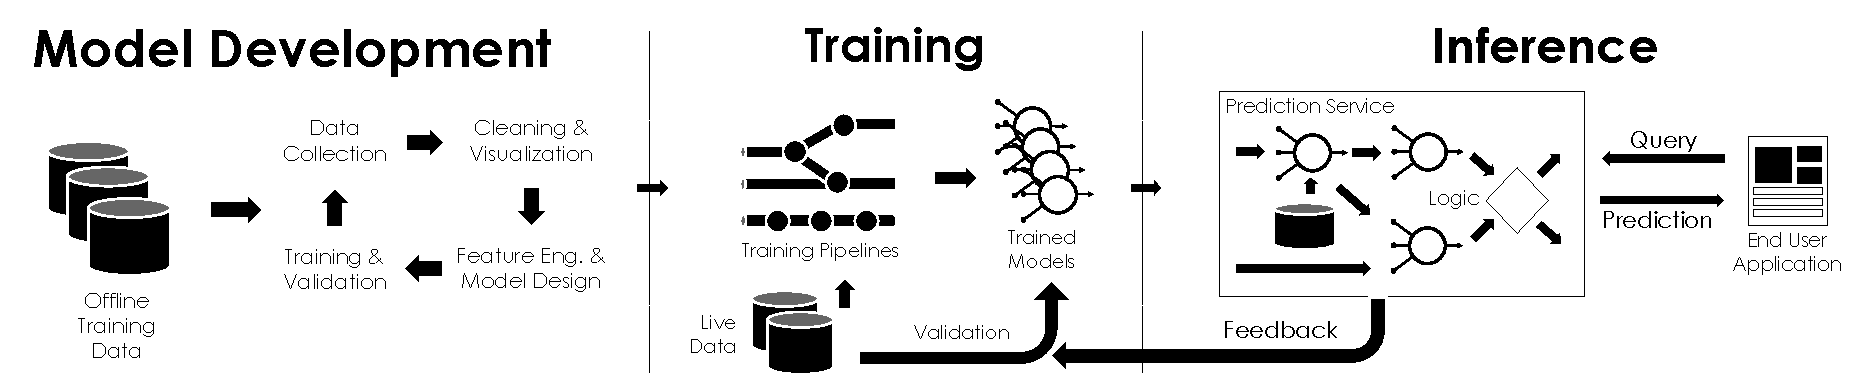
\includegraphics[width=\textwidth]{letters/pipeline.pdf}
\caption{\small \textbf{Machine Learning Life-cycle.} A simplified depiction of the key stages of a machine learning application.}
\label{fig:mllc}
\end{figure}


The machine learning life-cycle (Fig.~\ref{fig:mllc}) spans not only the model development, but also production training and inference.
Each stage demands different skills (e.g., neural network design, data management, and cluster management) and imposes different requirements on the underlying systems.
Yet there is an overwhelming need for unifying design principles and technologies to address pervasive problems including: feature management, data provenance, pipeline reproducibility, low-latency serving, and prediction monitoring just to name a few.


There has been substantial recent progress in systems to aid in managing the machine learning life-cycle.  
Large industrial projects like 
FB Learner Flow 
% \href{https://code.fb.com/core-data/introducing-fblearner-flow-facebook-s-ai-backbone/}{FB Learner Flow}
from Facebook, 
Michelangelo 
% \href{https://eng.uber.com/michelangelo/}{Michelangelo} 
from Uber, and 
TFX 
% \href{https://www.tensorflow.org/tfx/}{TFX} 
from Google have received a considerable of recent attention.  
In this issue we have solicited publications from several more recent industrial and academic projects.

The first paper, by a team at Amazon Research, provides an overview of several real-world use cases and then outlines the key conceptual, data management, and engineering challenges faced in production machine learning systems.
Rather than advocating a single system, this work describes some design principles that can inform potential solutions.


The second and third papers explores the challenges of model management and provenance across the machine learning life-cycle.
They motivate the need for systems to track models and their meta-data to improve reproducibility, collaboration, and governance. 
% expands upon the machine learning life-cycle 
% to include: data preparation, feature engineering, model training, deployment, and maintenance
% and explores the challenges of model 
The second paper introduces, ModelDB, an open-source system for model management and describe some of the functionality and design decisions. 
The third paper describes a related system, ProvDB, that uses a graph data model to capture and query fine-grained versioned lineage of data, scripts, and artifacts throughout the data analysis process.


The fourth paper, by a team at Databricks Inc., describes, MLFlow, a new open-source system to address the challenges of experimentation, reproducibility, and deployment. 
This work leverages containerization to capture the model development environment and a simple tracking API to enable experiment tracking.
The extensible model containerization enables model developers to more easily collaborate around modeling environments and then deploy model containers.


The last paper, by a team at Microsoft, focuses on inference and explores the challenges and opportunities of serving white-box prediction pipelines.  
In contrast to the containerization of pipelines in MLFlow, the Microsoft team leverage knowledge about the internal of the prediction pipeline to more efficient serve predictions. 



\end{document}



\end{letter}

\end{lettersection}



% put the name of your special issue below
\begin{articlesection}{Machine Learning Life-cycle Management}
%
%  Contributed articles section.  Use the articlesection environment.
%  Each article is contained in an article environment, where the two required
%  options to \begin{article} are the title and author of the article
%
%\begin{article}
%{Title of article}
%{list of authors}
%\input{author-name/article.tex}
%\end{article}
\begin{article}
{Toward Intelligent Query Engines}
{Matthaios Olma,  Stella Giannakopoulou,  Manos Karpathiotakis, Anastasia Ailamaki}
\graphicspath{{submissions/adaptivedb/}}
\pdfminorversion=5
\documentclass[11pt]{article}
\usepackage{deauthor,times,graphicx,caption,microtype}
\usepackage{hyperref}
\usepackage{listings}
\usepackage{booktabs}

\begin{document}

\title{Optimistic Lock Coupling: A Scalable and Efficient General-Purpose Synchronization Method}

\author{Viktor Leis, Michael Haubenschild\raisebox{0.9ex}{$\ast$}, Thomas Neumann\\ Technische Universit{\"a}t M{\"u}nchen \hspace{0.7cm} Tableau Software\raisebox{0.9ex}{$\ast$} \\ {\{leis,neumann\}{@}in.tum.de} \hspace{0.7cm} {mhaubenschild{@}tableau.com\raisebox{0.9ex}{$\ast$}}}

\maketitle

\begin{abstract}
As the number of cores on commodity processors continues to increase, scalability becomes more and more crucial for overall performance.
Scalable and efficient concurrent data structures are particularly important, as these are often the building blocks of parallel algorithms.
Unfortunately, traditional synchronization techniques based on fine-grained locking have been shown to be unscalable on modern multi-core CPUs.
Lock-free data structures, on the other hand, are extremely difficult to design and often incur significant overhead.

In this work, we make the case for Optimistic Lock Coupling as a practical alternative to both traditional locking and the lock-free approach.
We show that Optimistic Lock Coupling is highly scalable and almost as simple to implement as traditional lock coupling.
Another important advantage is that it is easily applicable to most tree-like data structures.
We therefore argue that Optimistic Lock Coupling, rather than a complex and error-prone custom synchronization protocol, should be the default choice for performance-critical data structures.
\end{abstract}

\section{Introduction}

% more and more cores
Today, Intel's commodity server processors have up to 28 cores and its upcoming microarchitecture will have up to 48 cores per socket~\cite{intel}.
Similarly, AMD currently stands at 32 cores and this number is expected to double in the next generation~\cite{amd}.
Since both platforms support simultaneous multithreading (also known as hyperthreading), affordable commodity servers (with up to two sockets) will soon routinely have between 100 and 200 hardware threads.

% data structure scalability is important
With such a high degree of hardware parallelism, efficient data processing crucially depends on how well concurrent data structures scale.
Internally, database systems use a plethora of data structures like table heaps, internal work queues, and, most importantly, index structures.
Any of these can easily become a scalability (and therefore overall performance) bottleneck on many-core CPUs.

% traditional synchronization: fine-grained locks, slow, cache invalidation
Traditionally, database systems synchronize internal data structures using fine-grained reader/writer locks\footnote{In this work, we focus on data structure synchronization rather than high-level transaction semantics and therefore use the term {\em lock} for what would typically be called {\em latch} in the database literature. We thus follow common computer science (rather than database) terminology.}.
Unfortunately, while fine-grained locking makes lock contention unlikely, it still results in bad scalability because lock acquisition and release require writing to shared memory.
Due to the way cache coherency is implemented on modern multi-core CPUs, these writes cause additional cache misses\footnote{The cache coherency protocol ensures that all copies of a cache line on other cores are invalidated before the write can proceed.} and the cache line containing the lock's internal data becomes a point of physical contention.
As a result, any frequently-accessed lock (e.g., the lock of the root node of a B-tree) severely limits scalability.

% lock-free bw-tree: no more latches, but indirections, extremely complex
Lock-free data structures like the Bw-tree~\cite{DBLP:conf/icde/LevandoskiLS13a} (a lock-free B-tree variant) or the Split-Ordered List~\cite{DBLP:journals/jacm/ShalevS06} (a lock-free hash table) do not acquire any locks and therefore generally scale much better than locking-based approaches (in particular for read-mostly workloads).
However, lock-free synchronization has other downsides:
First, it is very difficult and results in extremely complex and error-prone code (when compared to locking).
Second, because the functionality of atomic primitives provided by the hardware (e.g., atomically compare-and-swap 8 bytes) is limited, complex operations require additional indirections within the data structure.
For example, the Bw-tree requires an indirection table and the Split-Ordered List requires ``dummy nodes'', resulting in overhead due to additional cache misses.

% OLC for the win
In this paper we make the case for {\em Optimistic Lock Coupling (OLC)}, a synchronization method that combines some of the best properties of lock-based and lock-free synchronization.
OLC utilizes a special lock type that can be used in two modes:
The first mode is similar to a traditional mutex and excludes other threads by physically acquiring the underlying lock.
In the second mode, reads can proceed optimistically by validating a version counter that is embedded in the lock (similar to optimistic concurrency control).
The first mode is typically used by writers and the second mode by readers.
Besides this special lock type, OLC is based on the observation that optimistic lock validations can be interleaved/coupled---similar to the pair-wise interleaved lock acquisition of traditional lock coupling.
Hence, the name Optimistic Lock Coupling.

OLC has a number of desirable features:
\begin{itemize}
\item By reducing the number of writes to shared memory locations and thereby avoiding cache invalidations, it {\bf scales well} for most workloads.
\item In comparison to unsynchronized code, it requires few additional CPU instructions making it {\bf efficient}.
\item OLC is {\bf widely applicable} to different data structures. It has already been successfully used for synchronizing binary search trees~\cite{DBLP:conf/ppopp/BronsonCCO10}, tries~\cite{artsync}, trie/B-tree hybrids~\cite{DBLP:dblp_conf/eurosys/MaoKM12}, and B-trees~\cite{buzzword}.
\item In comparison to the lock-free paradigm, it is also {\bf easy to use} and requires few modifications to existing, single-threaded data structures.
\end{itemize}
Despite these positive features and its simplicity, OLC is not yet widely known.
The goal of this paper is therefore to popularize this simple idea and to make a case for it.
We argue that OLC deserves to be widely known.
It is a good default synchronization paradigm---more complex, data structure-specific protocols are seldom beneficial.

The rest of the paper is organized as follows.
Section~\ref{sec:related} discusses related work, tracing the history of OLC and its underlying ideas in the literature.
The core of the paper is Section~\ref{sec:olc}, which describes the ideas behind OLC and how it can be used to synchronize complex data structures.
In Section~\ref{sec:evaluation} we experimentally show that OLC has low overhead and scales well when used to synchronize an in-memory B-tree.
We summarize the paper in Section~\ref{sec:conc}.

\newpage
\section{Related Work}\label{sec:related}

Lock coupling has been proposed as a method for allowing concurrent operations on B-trees in 1977~\cite{DBLP:journals/acta/BayerS77}.
This traditional and still widely-used method, described in detail in Graefe's B-tree survey~\cite{DBLP:journals/ftdb/Graefe11}, is also called ``latch coupling'', ``hand-over-hand locking'', and ``crabbing''.
Because at most two locks are held at-a-time during tree traversal, this technique seemingly allows for a high degree of parallelism---in particular if read/write locks are used to enable inner nodes to be locked in shared mode.
However, as we show in Section~\ref{sec:evaluation}, on modern hardware lock acquisition (even in shared mode) results in suboptimal scalability.

An early alternative from 1981 is a B-tree variant called B-link tree~\cite{DBLP:journals/tods/LehmanY81}, which only holds a single lock at a time.
It is based on the observation that between the release of the parent lock and the acquisition of the child lock, the only ``dangerous'' thing that could have happened is the split of a child node (assuming one does not implement merge operations).
Thus, when a split happens, the key being searched might end up on a neighboring node to the right of the current child node.
A B-link tree traversal therefore detects this condition and, if needed, transparently proceeds to the neighboring node.
Releasing the parent lock early is highly beneficial when the child node needs to be fetched from disk.
For in-memory workloads, however, the B-link tree has the same scalability issues as lock coupling (it acquires just as many locks).

The next major advance, Optimistic Latch-Free Index Traversal (OLFIT)~\cite{DBLP:conf/vldb/ChaHKK01}, was proposed in 2001.
OLFIT introduced the idea of a combined lock/update counter, which we call {\em optimistic lock}. % , for lack of a better name,
Based on these per-node optimistic locks and the synchronization protocol of the B-link tree, OLFIT finally achieves good scalability on parallel processors.
The OLFIT protocol is fairly complex, as it requires both the non-trivial B-link protocol and optimistic locks.
Furthermore, like the B-link tree protocol, it does not support merging nodes, and is specific to B-trees (cannot easily be applied to other data structures).

In the following two decades, the growth of main-memory capacity led to much research into other data structures besides the venerable B-tree.
Particularly relevant for our discussion is Bronson et al.'s~\cite{DBLP:conf/ppopp/BronsonCCO10} concurrent binary search tree, which is based on optimistic version validation and has a sophisticated, data structure-specific synchronization protocol.
To the best of our knowledge, this 2010 paper is the first that, as part of its protocol, interleaves version validation across nodes---rather than validating each node separately like OLFIT.
In that paper, this idea is called ``hand-over-hand, optimistic validation'', while we prefer the term Optimistic Lock Coupling to highlight the close resemblance to traditional lock coupling.
Similarly, Mao et al.'s~\cite{DBLP:dblp_conf/eurosys/MaoKM12} Masstree (a concurrent hybrid trie/B-tree) is also based on the same ideas, but again uses them as part of a more complex protocol.

The Adaptive Radix Tree (ART)~\cite{art} is another recent in-memory data structure, which we proposed in 2013.
In contrast to the two data structures just mentioned, it was originally designed with single-threaded performance in mind without supporting concurrency.
To add support for concurrency, we initially started designing a custom protocol called Read-Optimized Write Exclusion (ROWEX)~\cite{artsync}, which turned out to be non-trivial and requires modifications of the underlying data structure\footnote{Note that ROWEX is already easier to apply to existing data structures than the lock-free approach. The difficulty depends on the data structure. Applying ROWEX is hard for B-trees with sorted keys and fairly easy for copy-on-write data structures like the Height Optimized Trie~\cite{hot}---with ART being somewhere in the middle.}.
However, fairly late in the project, we also realized, that OLC {\em alone} (rather than as part of a more complex protocol) is sufficient to synchronize ART.
No other changes to the data structure were necessary.
Both approaches were published and experimentally evaluated in a followup paper~\cite{artsync}, which shows that, despite its simplicity, OLC is efficient, scalable, and generally outperforms ROWEX.

Similar results were recently published regarding B-trees~\cite{buzzword}.
In this experimental study a simple OLC-based synchronization outperformed the Bw-tree~\cite{DBLP:conf/icde/LevandoskiLS13a}, a complex lock-free synchronization approach.
Another recent paper shows that for write-intensive workloads, locking often performs better than lock-free synchronization~\cite{DBLP:conf/cidr/FaleiroA17}.
These experiences indicate that OLC is a general-purpose synchronization paradigm and motivate the current paper.

%foster b-tree\cite{DBLP:journals/tods/GraefeKK12}
%Shasha theory~\cite{DBLP:journals/tods/ShashaG88}

\section{Optimistic Lock Coupling}\label{sec:olc}

% locks suck
The standard technique for inter-thread synchronization is mutual exclusion using fine-grained locks.
In a B-tree, for example, every node usually has its own associated lock, which is acquired before accessing that node.
The problem of locking on modern multi- and many-core processors is that lock acquisition and release require writing to the shared memory location that implements the lock.
This write causes exclusive ownership of the underlying cache line and invalidates copies of it on all other processor cores.
For hierarchical, tree-like data structures, the lock of the root node becomes a point of physical contention---even in read-only workloads and even when read/write locks are used.
Depending on the specific data structure, number of cores, cache coherency protocol implementation, cache topology, whether Non-Uniform Memory Access (NUMA) is used, locking can even result in multi-threaded performance that is worse than single-threaded execution.

% in b-trees this happens very much
The inherent pessimism of locking is particularly unfortunate for B-trees:
Despite the fact that logical modifications of the root node are very infrequent, every B-tree operation must lock the root node during tree traversal\footnote{To a lesser extent this obviously applies to all inner nodes, not just the root.}.
Even the vast majority of update operations (with the exception of splits and merges), only modify a single leaf node.
These observations indicate that a more optimistic approach, which does not require locking inner nodes, would be very beneficial for B-trees.

\subsection{Optimistic Locks}

% optimism to the rescue
As the name indicates, optimistic locks try to solve the scalability issues of traditional locks using an optimistic approach.
Instead of always physically acquiring locks, even for nodes that are unlikely to be modified simultaneously, after-the-fact validation is used to detect conflicts.
This is done by augmenting each lock with a version/update counter that is incremented on every modification.
Using this version counter, readers can optimistically proceed before validating that the version did not change to ensure that the read was safe.
If validation fails, the operation is restarted.

% details on opt locks
Using optimistic locks, a read-only node access (i.e., the majority of all operations in a B-tree) does not acquire the lock and does not increment the version counter.
Instead, it performs the following steps:
\begin{enumerate}
\item read lock version (restart if lock is not free)
\item access node
\item read the version again and validate that it has not changed in the meantime
\end{enumerate}
If the last step (the validation) fails, the operation has to be restarted.
Write operations, on the other hand, are more similar to traditional locking:
\begin{enumerate}
\item acquire lock (wait if necessary)
\item access/write to node
\item increment version and unlock node
\end{enumerate}
Writes can therefore protect a node from other writes.

% similar to locks
As we observed in an earlier paper~\cite{artsync}, because of similar semantics, optimistic locks can be hidden behind an API very similar to traditional read/write locks.
Both approaches have an exclusive lock mode, and acquiring a traditional lock in shared mode is analogous to optimistic version validation.
Furthermore, like with some implementations of traditional read/write locks, optimistic locks allow upgrading a shared lock to an exclusive lock.
Lock upgrades are, for example, used to avoid most B-tree update operations from having to lock inner nodes.
In our experience, the close resemblance of optimistic and traditional locks simplifies the reasoning about optimistic locks;
one can apply similar thinking as in traditional lock-based protocols.

\subsection{Lock Coupling with Optimistic Locks}

\begin{figure}
  \centering
  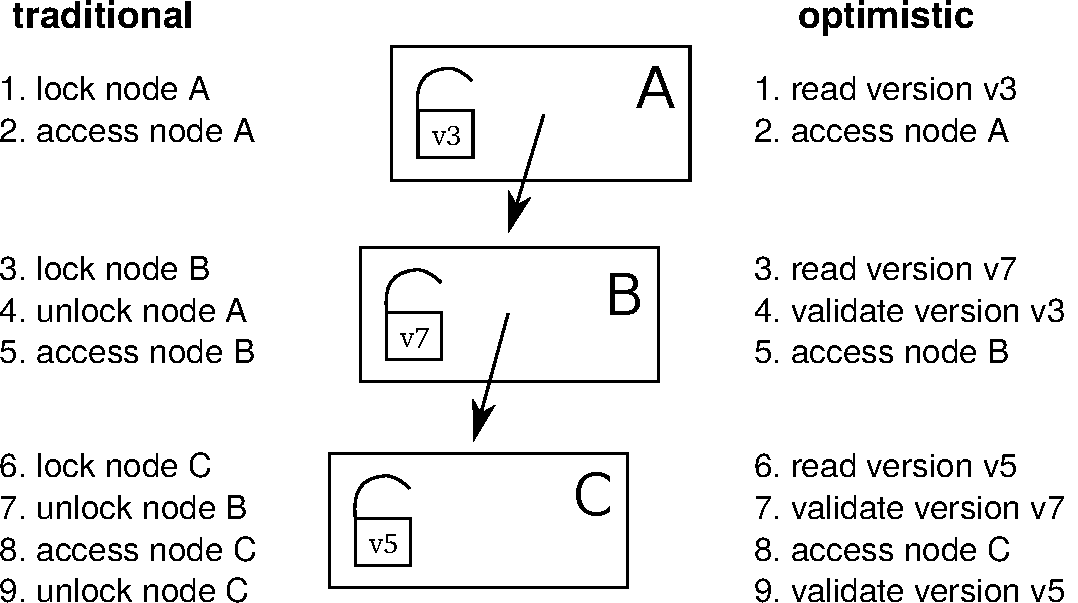
\includegraphics[width=0.65\linewidth]{olcall.pdf}
  \vspace{0.2cm}
  \caption{Comparison of a lookup operation in a 3-level tree using traditional lock coupling (left-hand side) vs.~optimistic lock coupling (right-hand side).}
  \label{fig:olc}
\end{figure}

The traditional and most common lock-based synchronization protocol for B-trees is lock coupling, which interleaves lock acquisitions while holding at most two locks at a time.
If, as we observed earlier, optimistic locks have similar semantics as traditional locks, it is natural to ask whether lock coupling can be combined with optimistic locks.
And indeed the answer is yes: One can almost mechanically translate traditional lock coupling code to optimistic lock coupling code.
This is illustrated in Figure~\ref{fig:olc}, which compares the traversal in a tree of height 3 using traditional and optimistic locks.
As the figure shows, the main difference is that locking is translated to reading the version and that unlocking becomes validation of the previously read version.
This simple change provides efficient lock-free tree traversal without the need to design a complex synchronization protocol.

It is important to emphasize the conceptual simplicity of OLC in comparison to data structures that use custom protocols like the Bw-tree~\cite{DBLP:conf/icde/LevandoskiLS13a}.
To implement lock-free access, the Bw-tree requires an indirection table, delta nodes, complex splitting and merging logic, retry logic, etc.
OLC, on the other hand, can directly be applied to B-trees mostly by adding the appropriate optimistic locking code and without modifying the node layout itself.
Therefore, OpenBw-Tree, an open source implementation of the Bw-tree, requires an order of magnitude more code than a B-tree based on OLC\footnote{Both implementations are available on GitHub: \url{https://github.com/wangziqi2016/index-microbench}}.
Given how difficult it is to develop, validate, and debug lock-free code, simplicity is obviously a major advantage.

\subsection{Correctness Aspects}

\begin{figure}
  % \centering
  %[basicstyle=\normalsize\ttfamily,showstringspaces=false,columns=fullflexible,breaklines=false,breakatwhitespace=true,numbers=none,numberstyle=\small,style=C,keepspaces=true]
\begin{lstlisting}[basicstyle=\ttfamily,language=C++,numbers=left,numberstyle=\small]
std::atomic<BTreeNode*> root;

// search for key in B+tree, returns payload in resultOut
bool lookup(Key key, Value& resultOut) {
   BTreeNode* node = root.load();
   uint64_t nodeVersion = node->readLockOrRestart();
   if (node != root.load()) // make sure the root is still the root
      restart();

   BTreeInner<Key>* parent = nullptr;
   uint64_t parentVersion = 0;

   while (node->isInner()) {
      auto inner = (BTreeInner*)node;

      // unlock parent and make current node the parent
      if (parent)
         parent->readUnlockOrRestart(parentVersion);
      parent = inner;
      parentVersion = nodeVersion;

      // search for next node
      node = inner->findChild(key);
      // validate 'inner' to ensure that 'node' pointer is valid
      inner->checkOrRestart(nodeVersion);
      // now it safe to dereference 'node' pointer (read its version)
      nodeVersion = node->readLockOrRestart();
   }

   // search in leaf and retrieve payload
   auto leaf = (BTreeLeaf*)node;
   bool success = leaf->findValue(key, resultOut);

   // unlock everything
   if (parent)
      parent->readUnlockOrRestart(parentVersion);
   node->readUnlockOrRestart(nodeVersion);

   return success;
}
\end{lstlisting}
  \vspace{0.2cm}
  \caption{B-tree lookup code using OLC. For simplicity, the restart logic is not shown.}
  \label{fig:lookup}
\end{figure}

So far, we have introduced the high-level ideas behind OLC and have stressed its similarity to traditional lock coupling.
Let us now discuss some cases where the close similarity between lock coupling and OLC breaks down.
To make this more concrete, we show the B-tree lookup code in Figure~\ref{fig:lookup}.
In the code, \texttt{readLockOrRestart} reads the lock version and \texttt{readUnlockOrRestart} validates that the read was correct.

One issue with OLC is that any pointer speculatively read from a node may point to invalid memory (if that node is modified concurrently).
Dereferencing such a pointer (e.g., to read its optimistic lock), may cause a segmentation fault or undefined behavior.
In the code shown in Figure~\ref{fig:lookup}, this problem is prevented by the extra check in line 25, which ensures that the read from the node containing the pointer was correct.
Without this additional validation, the code would in line 27 dereference the pointer speculatively read in line 23.
Note that the implementation of \texttt{checkOrRestart} is actually identical to \texttt{readUnlockOrRestart}.
We chose to give it a different name to highlight the fact that this extra check would not be necessary with read/write locks.

Another potential issue with optimistic locks is code that does not terminate.
Code that speculatively accesses a node, like an intra-node binary search, should be written in a way such that it always terminates---even in the presence of concurrent writes.
Otherwise, the validation code that detects the concurrent write will never run.
The binary search of a B-tree, for example, needs to be written in such a way that each comparison makes progress.
For some data structures that do not require loops in the traversal code (like ART) termination is trivially true.

\subsection{Implementation Details}

% implementation, efficiency
To implement an optimistic lock, one can combine the lock and the version counter into a single 64-bit\footnote{Even after subtracting one bit for the lock status, a back-of-the-envelope calculation can show that 63 bits are large enough to never overflow in practice.} word~\cite{artsync}.
A typical read operation will therefore merely consist of reading this version counter atomically.
In C++11 this can be implemented using the \texttt{std::atomic} type.

On x86, atomic reads are cheap because of x86's strong memory order guarantees.
No memory fences are required for sequentially-consistent loads, which are translated (by both GCC and clang) into standard \texttt{MOV} instructions.
Hence, the only effect of \texttt{std::atomic} for loads is preventing instruction re-ordering.
This makes version access and validation cheap.
Acquiring and releasing an optimistic lock in exclusive mode has comparable cost to a traditional lock:
A fairly expensive sequentially-consistent store is needed for acquiring a lock, while a standard \texttt{MOV} suffices for releasing it.
A simple sinlock-based implementation of optimistic locks can be found in the appendix of an earlier paper~\cite{artsync}.

OLC code must be able to handle restarts since validation or lock upgrade can fail due to concurrent writers.
Restarts can easily be implemented by wrapping the data structure operation in a loop (for simplicity not shown in Figure~\ref{fig:lookup}).
Such a loop also enables limiting the number of optimistic retry operations and falling back to pessimistic locking in cases of very heavy contention.
The ability to fall back to traditional locking is a major advantage of OLC in terms of robustness over lock-free approaches, which do not have this option.

In addition to the optimistic shared mode and the exclusive mode, optimistic locks also support a ``shared pessimistic'' mode, which physically acquires the lock in shared mode (allowing multiple concurrent readers but no writers).
This mode is useful for table (or range) scans that touch many tuples on a leaf page (which would otherwise easily abort).
Finally, let us mention that large range scans and table scans, should be broken up into several per-node traversals as is done in the LeanStore~\cite{leanstore} system.

Like all lock-free data structures, but unlike traditional locking and Hardware Transactional Memory~\cite{DBLP:conf/hpca/KarnagelDRLLSL14,DBLP:journals/pvldb/MakreshanskiLS15,htmtkde}, OLC requires care when deleting (and reusing) nodes.
The reason is that a deleting thread can never be sure that a node can be reclaimed because other threads might still be optimistically reading from that node.
Therefore, standard solutions like epoch-based reclamation~\cite{DBLP:conf/sosp/TuZKLM13}, hazard pointers~\cite{DBLP:journals/tpds/Michael04}, or optimized hazard pointers~\cite{DBLP:conf/spaa/BalmauGHZ16} need to be used.
These memory reclamation techniques are, however, largely orthogonal to the synchronization protocol itself.

%-lock-free is not a strong guarantee

\newpage
\section{Evaluation}\label{sec:evaluation}

Let us now experimentally evaluate the overhead and scalability of OLC.
For the experiments, we use an in-memory B+tree implemented in C++11 using templates, which is configured to use nodes of 4096 bytes, random 8 byte keys, and 8 byte payloads.
Based on this B-tree, we compare the following synchronization approaches:
\begin{itemize}
\item an OLC implementation\footnote{An almost identical OLC implementation is available on github: \url{https://github.com/wangziqi2016/index-microbench/tree/master/BTreeOLC}}
\item a variant based on traditional lock coupling and read/write locks
\item the unsynchronized B-tree, which obviously is only correct for read-only workloads but allows measuring the overhead of synchronization
\end{itemize}
Note that earlier work has compared the OLC implementation with a Bw-tree implementation~\cite{buzzword} and other state-of-the-art in-memory index structures.

We use a Haswell EP system with an Intel Xeon E5-2687W v3 CPU, which has 10 cores (20 ``Hyper-Threads'') and 25~MB of L3 cache.
The system is running Ubuntu 18.10 and we use GCC 8.2.0 to compile our code.
The CPU counters are obtained using the Linux perf API\footnote{We use the following convenience wrapper: \url{https://github.com/viktorleis/perfevent}}.

\begin{table}
  \caption{Performance and CPU counters for lookup and insert operations in a B-tree with 100M keys. We perform 100M operations and normalize the CPU counters by that number.}
  \label{tab:overhead}
  \centering
  \begin{tabular}{lrrrrrrr}\toprule
                    &         &        &        & instruc-  & L1     & L3     & branch \\
                    & threads & M op/s & cycles & tions & misses & misses & misses \\\midrule
lookup (no sync.)   & 1       & 1.72   & 2028   & 283     & 39.1   & 14.9   & 16.1   \\
lookup (OLC)        & 1       & 1.65   & 2107   & 370     & 43.9   & 15.1   & 16.7   \\
lookup (lock coup.) & 1       & 1.72   & 2078   & 365     & 42.3   & 16.9   & 15.7   \\\midrule
insert (no sync.)   & 1       & 1.51   & 2286   & 530     & 59.8   & 31.1   & 17.3   \\
insert (OLC)        & 1       & 1.50   & 2303   & 629     & 61.2   & 31.1   & 16.5   \\
insert (lock coup.) & 1       & 1.41   & 2473   & 644     & 61.0   & 31.0   & 17.2   \\\midrule
lookup (no sync.)   & 10      & 15.48  & 2058   & 283     & 38.6   & 15.5   & 16.0   \\
lookup (OLC)        & 10      & 14.60  & 2187   & 370     & 43.8   & 15.8   & 16.8   \\
lookup (lock coup.) & 10      & 5.71   & 5591   & 379     & 54.2   & 17.0   & 14.8   \\\midrule
insert (no sync.)   & 10      & -      & -      & -       & -      & -      & -      \\
insert (OLC)        & 10      & 10.46  & 2940   & 656     & 62.0   & 32.5   & 16.8   \\
insert (lock coup.) & 10      & 7.55   & 4161   & 667     & 75.0   & 28.6   & 16.2   \\
    \bottomrule
\end{tabular}
\end{table}

Table~\ref{tab:overhead} compares the performance and CPU counters for lookup and insert operations in a B-tree with 100M keys.
With {\em single-threaded} execution, we observe that all three approaches have very similar performance.
Adding traditional or optimistic locks to unsynchronized B-tree code results in up to 30\% of additional instructions without affecting single-threaded performance much.

\begin{figure}
  \centering
  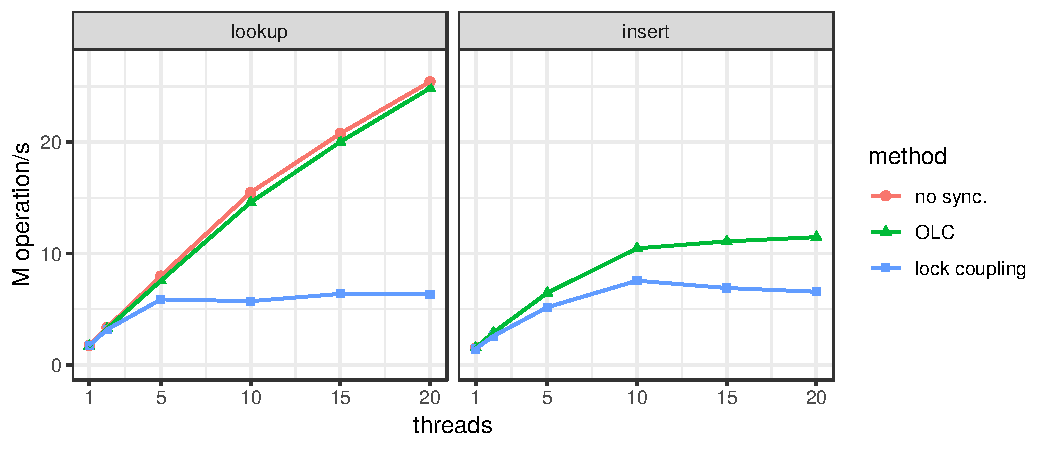
\includegraphics[width=\linewidth]{scale.pdf}
  \vspace{0.2cm}
  \caption{Scalability on 10-core system for B-tree operations (100M values).}
  \label{fig:scale}
\end{figure}

As Figure~\ref{fig:scale} shows, the results change dramatically once we use multiple threads.
For lookup, the scalability of OLC is near-linear up to 20 threads, even though the system has only 10 ``real cores''.
The OLC scalability for insert is also respectable (though not quite as linear because multi-threaded insertion approaches the memory bandwidth of our processor).
The figure also shows that the results of traditional lock coupling with read/write locks are significantly worse than OLC.
With 20 threads, lookup with OLC is 3.9$\times$ faster than traditional lock coupling.

\section{Summary}\label{sec:conc}

Optimistic Lock Coupling (OLC) is an effective synchronization method that combines the simplicity of traditional lock coupling with the superior scalability of lock-free approaches.
OLC is widely applicable and has already been successfully used to synchronize several data structures, including B-trees, binary search trees, and different trie variants.
These features make it highly attractive for modern database systems as well as performance-critical systems software in general.

\begin{thebibliography}{10}

\bibitem{DBLP:conf/spaa/BalmauGHZ16}
O.~Balmau, R.~Guerraoui, M.~Herlihy, and I.~Zablotchi.
\newblock Fast and robust memory reclamation for concurrent data structures.
\newblock In {\em SPAA}, 2016.

\bibitem{DBLP:journals/acta/BayerS77}
R.~Bayer and M.~Schkolnick.
\newblock Concurrency of operations on {B}-trees.
\newblock {\em Acta Informatica}, 9, 1977.

\bibitem{hot}
R.~Binna, E.~Zangerle, M.~Pichl, G.~Specht, and V.~Leis.
\newblock {HOT}: A height optimized trie index for main-memory database
  systems.
\newblock In {\em SIGMOD}, 2018.

\bibitem{DBLP:conf/ppopp/BronsonCCO10}
N.~G. Bronson, J.~Casper, H.~Chafi, and K.~Olukotun.
\newblock A practical concurrent binary search tree.
\newblock In {\em PPOPP}, 2010.

\bibitem{DBLP:conf/vldb/ChaHKK01}
S.~K. Cha, S.~Hwang, K.~Kim, and K.~Kwon.
\newblock Cache-conscious concurrency control of main-memory indexes on
  shared-memory multiprocessor systems.
\newblock In {\em VLDB}, 2001.

\bibitem{intel}
I.~Cutress.
\newblock {Intel} goes for 48-cores: {Cascade-AP} with multi-chip package
  coming soon.
\newblock
  \url{https://www.anandtech.com/show/13535/intel-goes-for-48cores-cascade-ap},
  2018 (accessed January, 2019).

\bibitem{DBLP:conf/cidr/FaleiroA17}
J.~M. Faleiro and D.~J. Abadi.
\newblock Latch-free synchronization in database systems: Silver bullet or
  fool's gold?
\newblock In {\em CIDR}, 2017.

\bibitem{DBLP:journals/ftdb/Graefe11}
G.~Graefe.
\newblock Modern {B}-tree techniques.
\newblock {\em Foundations and Trends in Databases}, 3(4), 2011.

\bibitem{DBLP:conf/hpca/KarnagelDRLLSL14}
T.~Karnagel, R.~Dementiev, R.~Rajwar, K.~Lai, T.~Legler, B.~Schlegel, and
  W.~Lehner.
\newblock Improving in-memory database index performance with
  {Intel}\({}^{\mbox{{\textregistered}}}\) transactional synchronization
  extensions.
\newblock In {\em HPCA}, 2014.

\bibitem{DBLP:journals/tods/LehmanY81}
P.~L. Lehman and S.~B. Yao.
\newblock Efficient locking for concurrent operations on {B}-trees.
\newblock {\em {ACM} Trans. Database Syst.}, 6(4), 1981.

\bibitem{leanstore}
V.~Leis, M.~Haubenschild, A.~Kemper, and T.~Neumann.
\newblock Leanstore: In-memory data management beyond main memory.
\newblock In {\em ICDE}, 2018.

\bibitem{art}
V.~Leis, A.~Kemper, and T.~Neumann.
\newblock The adaptive radix tree: {ARTful} indexing for main-memory databases.
\newblock In {\em ICDE}, 2013.

\bibitem{htmtkde}
V.~Leis, A.~Kemper, and T.~Neumann.
\newblock Scaling {HTM}-supported database transactions to many cores.
\newblock {\em {IEEE} Trans. Knowl. Data Eng.}, 28(2), 2016.

\bibitem{artsync}
V.~Leis, F.~Scheibner, A.~Kemper, and T.~Neumann.
\newblock The {ART} of practical synchronization.
\newblock In {\em DaMoN}, 2016.

\bibitem{DBLP:conf/icde/LevandoskiLS13a}
J.~J. Levandoski, D.~B. Lomet, and S.~Sengupta.
\newblock The {Bw}-tree: A {B}-tree for new hardware platforms.
\newblock In {\em ICDE}, 2013.

\bibitem{DBLP:journals/pvldb/MakreshanskiLS15}
D.~Makreshanski, J.~J. Levandoski, and R.~Stutsman.
\newblock To lock, swap, or elide: On the interplay of hardware transactional
  memory and lock-free indexing.
\newblock {\em {PVLDB}}, 8(11), 2015.

\bibitem{DBLP:dblp_conf/eurosys/MaoKM12}
Y.~Mao, E.~Kohler, and R.~T. Morris.
\newblock Cache craftiness for fast multicore key-value storage.
\newblock In {\em EuroSys}, 2012.

\bibitem{DBLP:journals/tpds/Michael04}
M.~M. Michael.
\newblock Hazard pointers: Safe memory reclamation for lock-free objects.
\newblock {\em {IEEE} Trans. Parallel Distrib. Syst.}, 15(6), 2004.

\bibitem{DBLP:journals/jacm/ShalevS06}
O.~Shalev and N.~Shavit.
\newblock Split-ordered lists: Lock-free extensible hash tables.
\newblock {\em J. {ACM}}, 53(3), 2006.

\bibitem{amd}
A.~Shilov.
\newblock {AMD} previews {EPYC} ‘{Rome}’ processor: Up to 64 {Zen} 2 cores.
\newblock
  \url{https://www.anandtech.com/show/13561/amd-previews-epyc-rome-processor-up-to-64-zen-2-cores},
  2018 (accessed January, 2019).

\bibitem{DBLP:conf/sosp/TuZKLM13}
S.~Tu, W.~Zheng, E.~Kohler, B.~Liskov, and S.~Madden.
\newblock Speedy transactions in multicore in-memory databases.
\newblock In {\em SOSP}, 2013.

\bibitem{buzzword}
Z.~Wang, A.~Pavlo, H.~Lim, V.~Leis, H.~Zhang, M.~Kaminsky, and D.~Andersen.
\newblock Building a {Bw}-tree takes more than just buzz words.
\newblock In {\em SIGMOD}, 2018.

\end{thebibliography}


%\bibliographystyle{abbrv}
%\bibliography{main}

\end{document}

\end{article}


\begin{article}
{doppioDB 1.0: Machine Learning inside a Relational Engine}
{Gustavo Alonso, Zsolt Istvan, Kaan Kara, Muhsen Owaida, David Sidler}
\graphicspath{{submissions/gustavo/}}
\pdfminorversion=5
\documentclass[11pt]{article}
\usepackage{deauthor,times,graphicx,caption,microtype}
\usepackage{hyperref}
\usepackage{listings}
\usepackage{booktabs}

\begin{document}

\title{Optimistic Lock Coupling: A Scalable and Efficient General-Purpose Synchronization Method}

\author{Viktor Leis, Michael Haubenschild\raisebox{0.9ex}{$\ast$}, Thomas Neumann\\ Technische Universit{\"a}t M{\"u}nchen \hspace{0.7cm} Tableau Software\raisebox{0.9ex}{$\ast$} \\ {\{leis,neumann\}{@}in.tum.de} \hspace{0.7cm} {mhaubenschild{@}tableau.com\raisebox{0.9ex}{$\ast$}}}

\maketitle

\begin{abstract}
As the number of cores on commodity processors continues to increase, scalability becomes more and more crucial for overall performance.
Scalable and efficient concurrent data structures are particularly important, as these are often the building blocks of parallel algorithms.
Unfortunately, traditional synchronization techniques based on fine-grained locking have been shown to be unscalable on modern multi-core CPUs.
Lock-free data structures, on the other hand, are extremely difficult to design and often incur significant overhead.

In this work, we make the case for Optimistic Lock Coupling as a practical alternative to both traditional locking and the lock-free approach.
We show that Optimistic Lock Coupling is highly scalable and almost as simple to implement as traditional lock coupling.
Another important advantage is that it is easily applicable to most tree-like data structures.
We therefore argue that Optimistic Lock Coupling, rather than a complex and error-prone custom synchronization protocol, should be the default choice for performance-critical data structures.
\end{abstract}

\section{Introduction}

% more and more cores
Today, Intel's commodity server processors have up to 28 cores and its upcoming microarchitecture will have up to 48 cores per socket~\cite{intel}.
Similarly, AMD currently stands at 32 cores and this number is expected to double in the next generation~\cite{amd}.
Since both platforms support simultaneous multithreading (also known as hyperthreading), affordable commodity servers (with up to two sockets) will soon routinely have between 100 and 200 hardware threads.

% data structure scalability is important
With such a high degree of hardware parallelism, efficient data processing crucially depends on how well concurrent data structures scale.
Internally, database systems use a plethora of data structures like table heaps, internal work queues, and, most importantly, index structures.
Any of these can easily become a scalability (and therefore overall performance) bottleneck on many-core CPUs.

% traditional synchronization: fine-grained locks, slow, cache invalidation
Traditionally, database systems synchronize internal data structures using fine-grained reader/writer locks\footnote{In this work, we focus on data structure synchronization rather than high-level transaction semantics and therefore use the term {\em lock} for what would typically be called {\em latch} in the database literature. We thus follow common computer science (rather than database) terminology.}.
Unfortunately, while fine-grained locking makes lock contention unlikely, it still results in bad scalability because lock acquisition and release require writing to shared memory.
Due to the way cache coherency is implemented on modern multi-core CPUs, these writes cause additional cache misses\footnote{The cache coherency protocol ensures that all copies of a cache line on other cores are invalidated before the write can proceed.} and the cache line containing the lock's internal data becomes a point of physical contention.
As a result, any frequently-accessed lock (e.g., the lock of the root node of a B-tree) severely limits scalability.

% lock-free bw-tree: no more latches, but indirections, extremely complex
Lock-free data structures like the Bw-tree~\cite{DBLP:conf/icde/LevandoskiLS13a} (a lock-free B-tree variant) or the Split-Ordered List~\cite{DBLP:journals/jacm/ShalevS06} (a lock-free hash table) do not acquire any locks and therefore generally scale much better than locking-based approaches (in particular for read-mostly workloads).
However, lock-free synchronization has other downsides:
First, it is very difficult and results in extremely complex and error-prone code (when compared to locking).
Second, because the functionality of atomic primitives provided by the hardware (e.g., atomically compare-and-swap 8 bytes) is limited, complex operations require additional indirections within the data structure.
For example, the Bw-tree requires an indirection table and the Split-Ordered List requires ``dummy nodes'', resulting in overhead due to additional cache misses.

% OLC for the win
In this paper we make the case for {\em Optimistic Lock Coupling (OLC)}, a synchronization method that combines some of the best properties of lock-based and lock-free synchronization.
OLC utilizes a special lock type that can be used in two modes:
The first mode is similar to a traditional mutex and excludes other threads by physically acquiring the underlying lock.
In the second mode, reads can proceed optimistically by validating a version counter that is embedded in the lock (similar to optimistic concurrency control).
The first mode is typically used by writers and the second mode by readers.
Besides this special lock type, OLC is based on the observation that optimistic lock validations can be interleaved/coupled---similar to the pair-wise interleaved lock acquisition of traditional lock coupling.
Hence, the name Optimistic Lock Coupling.

OLC has a number of desirable features:
\begin{itemize}
\item By reducing the number of writes to shared memory locations and thereby avoiding cache invalidations, it {\bf scales well} for most workloads.
\item In comparison to unsynchronized code, it requires few additional CPU instructions making it {\bf efficient}.
\item OLC is {\bf widely applicable} to different data structures. It has already been successfully used for synchronizing binary search trees~\cite{DBLP:conf/ppopp/BronsonCCO10}, tries~\cite{artsync}, trie/B-tree hybrids~\cite{DBLP:dblp_conf/eurosys/MaoKM12}, and B-trees~\cite{buzzword}.
\item In comparison to the lock-free paradigm, it is also {\bf easy to use} and requires few modifications to existing, single-threaded data structures.
\end{itemize}
Despite these positive features and its simplicity, OLC is not yet widely known.
The goal of this paper is therefore to popularize this simple idea and to make a case for it.
We argue that OLC deserves to be widely known.
It is a good default synchronization paradigm---more complex, data structure-specific protocols are seldom beneficial.

The rest of the paper is organized as follows.
Section~\ref{sec:related} discusses related work, tracing the history of OLC and its underlying ideas in the literature.
The core of the paper is Section~\ref{sec:olc}, which describes the ideas behind OLC and how it can be used to synchronize complex data structures.
In Section~\ref{sec:evaluation} we experimentally show that OLC has low overhead and scales well when used to synchronize an in-memory B-tree.
We summarize the paper in Section~\ref{sec:conc}.

\newpage
\section{Related Work}\label{sec:related}

Lock coupling has been proposed as a method for allowing concurrent operations on B-trees in 1977~\cite{DBLP:journals/acta/BayerS77}.
This traditional and still widely-used method, described in detail in Graefe's B-tree survey~\cite{DBLP:journals/ftdb/Graefe11}, is also called ``latch coupling'', ``hand-over-hand locking'', and ``crabbing''.
Because at most two locks are held at-a-time during tree traversal, this technique seemingly allows for a high degree of parallelism---in particular if read/write locks are used to enable inner nodes to be locked in shared mode.
However, as we show in Section~\ref{sec:evaluation}, on modern hardware lock acquisition (even in shared mode) results in suboptimal scalability.

An early alternative from 1981 is a B-tree variant called B-link tree~\cite{DBLP:journals/tods/LehmanY81}, which only holds a single lock at a time.
It is based on the observation that between the release of the parent lock and the acquisition of the child lock, the only ``dangerous'' thing that could have happened is the split of a child node (assuming one does not implement merge operations).
Thus, when a split happens, the key being searched might end up on a neighboring node to the right of the current child node.
A B-link tree traversal therefore detects this condition and, if needed, transparently proceeds to the neighboring node.
Releasing the parent lock early is highly beneficial when the child node needs to be fetched from disk.
For in-memory workloads, however, the B-link tree has the same scalability issues as lock coupling (it acquires just as many locks).

The next major advance, Optimistic Latch-Free Index Traversal (OLFIT)~\cite{DBLP:conf/vldb/ChaHKK01}, was proposed in 2001.
OLFIT introduced the idea of a combined lock/update counter, which we call {\em optimistic lock}. % , for lack of a better name,
Based on these per-node optimistic locks and the synchronization protocol of the B-link tree, OLFIT finally achieves good scalability on parallel processors.
The OLFIT protocol is fairly complex, as it requires both the non-trivial B-link protocol and optimistic locks.
Furthermore, like the B-link tree protocol, it does not support merging nodes, and is specific to B-trees (cannot easily be applied to other data structures).

In the following two decades, the growth of main-memory capacity led to much research into other data structures besides the venerable B-tree.
Particularly relevant for our discussion is Bronson et al.'s~\cite{DBLP:conf/ppopp/BronsonCCO10} concurrent binary search tree, which is based on optimistic version validation and has a sophisticated, data structure-specific synchronization protocol.
To the best of our knowledge, this 2010 paper is the first that, as part of its protocol, interleaves version validation across nodes---rather than validating each node separately like OLFIT.
In that paper, this idea is called ``hand-over-hand, optimistic validation'', while we prefer the term Optimistic Lock Coupling to highlight the close resemblance to traditional lock coupling.
Similarly, Mao et al.'s~\cite{DBLP:dblp_conf/eurosys/MaoKM12} Masstree (a concurrent hybrid trie/B-tree) is also based on the same ideas, but again uses them as part of a more complex protocol.

The Adaptive Radix Tree (ART)~\cite{art} is another recent in-memory data structure, which we proposed in 2013.
In contrast to the two data structures just mentioned, it was originally designed with single-threaded performance in mind without supporting concurrency.
To add support for concurrency, we initially started designing a custom protocol called Read-Optimized Write Exclusion (ROWEX)~\cite{artsync}, which turned out to be non-trivial and requires modifications of the underlying data structure\footnote{Note that ROWEX is already easier to apply to existing data structures than the lock-free approach. The difficulty depends on the data structure. Applying ROWEX is hard for B-trees with sorted keys and fairly easy for copy-on-write data structures like the Height Optimized Trie~\cite{hot}---with ART being somewhere in the middle.}.
However, fairly late in the project, we also realized, that OLC {\em alone} (rather than as part of a more complex protocol) is sufficient to synchronize ART.
No other changes to the data structure were necessary.
Both approaches were published and experimentally evaluated in a followup paper~\cite{artsync}, which shows that, despite its simplicity, OLC is efficient, scalable, and generally outperforms ROWEX.

Similar results were recently published regarding B-trees~\cite{buzzword}.
In this experimental study a simple OLC-based synchronization outperformed the Bw-tree~\cite{DBLP:conf/icde/LevandoskiLS13a}, a complex lock-free synchronization approach.
Another recent paper shows that for write-intensive workloads, locking often performs better than lock-free synchronization~\cite{DBLP:conf/cidr/FaleiroA17}.
These experiences indicate that OLC is a general-purpose synchronization paradigm and motivate the current paper.

%foster b-tree\cite{DBLP:journals/tods/GraefeKK12}
%Shasha theory~\cite{DBLP:journals/tods/ShashaG88}

\section{Optimistic Lock Coupling}\label{sec:olc}

% locks suck
The standard technique for inter-thread synchronization is mutual exclusion using fine-grained locks.
In a B-tree, for example, every node usually has its own associated lock, which is acquired before accessing that node.
The problem of locking on modern multi- and many-core processors is that lock acquisition and release require writing to the shared memory location that implements the lock.
This write causes exclusive ownership of the underlying cache line and invalidates copies of it on all other processor cores.
For hierarchical, tree-like data structures, the lock of the root node becomes a point of physical contention---even in read-only workloads and even when read/write locks are used.
Depending on the specific data structure, number of cores, cache coherency protocol implementation, cache topology, whether Non-Uniform Memory Access (NUMA) is used, locking can even result in multi-threaded performance that is worse than single-threaded execution.

% in b-trees this happens very much
The inherent pessimism of locking is particularly unfortunate for B-trees:
Despite the fact that logical modifications of the root node are very infrequent, every B-tree operation must lock the root node during tree traversal\footnote{To a lesser extent this obviously applies to all inner nodes, not just the root.}.
Even the vast majority of update operations (with the exception of splits and merges), only modify a single leaf node.
These observations indicate that a more optimistic approach, which does not require locking inner nodes, would be very beneficial for B-trees.

\subsection{Optimistic Locks}

% optimism to the rescue
As the name indicates, optimistic locks try to solve the scalability issues of traditional locks using an optimistic approach.
Instead of always physically acquiring locks, even for nodes that are unlikely to be modified simultaneously, after-the-fact validation is used to detect conflicts.
This is done by augmenting each lock with a version/update counter that is incremented on every modification.
Using this version counter, readers can optimistically proceed before validating that the version did not change to ensure that the read was safe.
If validation fails, the operation is restarted.

% details on opt locks
Using optimistic locks, a read-only node access (i.e., the majority of all operations in a B-tree) does not acquire the lock and does not increment the version counter.
Instead, it performs the following steps:
\begin{enumerate}
\item read lock version (restart if lock is not free)
\item access node
\item read the version again and validate that it has not changed in the meantime
\end{enumerate}
If the last step (the validation) fails, the operation has to be restarted.
Write operations, on the other hand, are more similar to traditional locking:
\begin{enumerate}
\item acquire lock (wait if necessary)
\item access/write to node
\item increment version and unlock node
\end{enumerate}
Writes can therefore protect a node from other writes.

% similar to locks
As we observed in an earlier paper~\cite{artsync}, because of similar semantics, optimistic locks can be hidden behind an API very similar to traditional read/write locks.
Both approaches have an exclusive lock mode, and acquiring a traditional lock in shared mode is analogous to optimistic version validation.
Furthermore, like with some implementations of traditional read/write locks, optimistic locks allow upgrading a shared lock to an exclusive lock.
Lock upgrades are, for example, used to avoid most B-tree update operations from having to lock inner nodes.
In our experience, the close resemblance of optimistic and traditional locks simplifies the reasoning about optimistic locks;
one can apply similar thinking as in traditional lock-based protocols.

\subsection{Lock Coupling with Optimistic Locks}

\begin{figure}
  \centering
  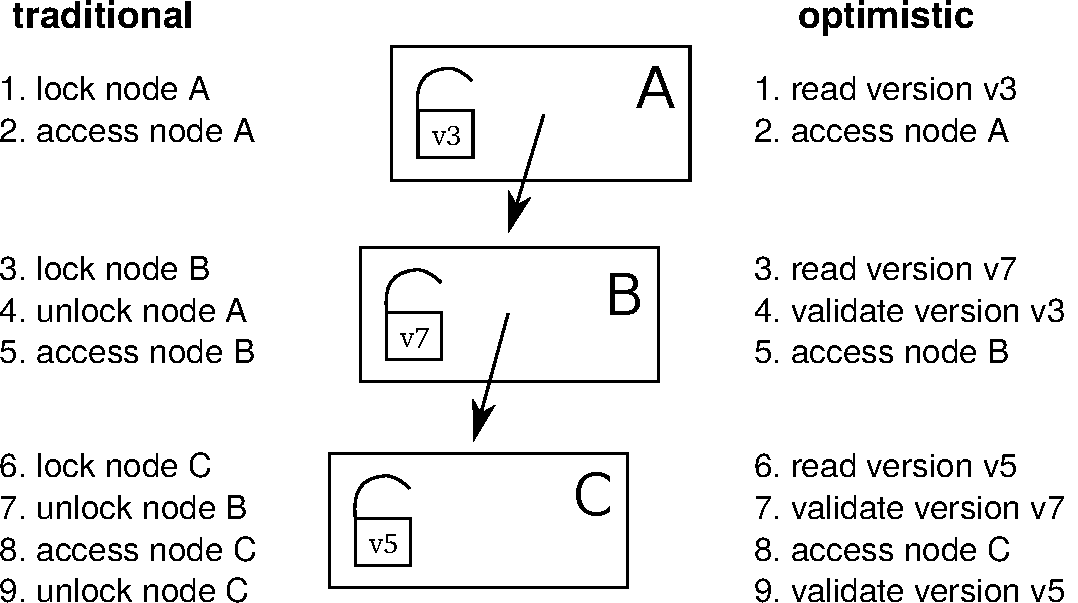
\includegraphics[width=0.65\linewidth]{olcall.pdf}
  \vspace{0.2cm}
  \caption{Comparison of a lookup operation in a 3-level tree using traditional lock coupling (left-hand side) vs.~optimistic lock coupling (right-hand side).}
  \label{fig:olc}
\end{figure}

The traditional and most common lock-based synchronization protocol for B-trees is lock coupling, which interleaves lock acquisitions while holding at most two locks at a time.
If, as we observed earlier, optimistic locks have similar semantics as traditional locks, it is natural to ask whether lock coupling can be combined with optimistic locks.
And indeed the answer is yes: One can almost mechanically translate traditional lock coupling code to optimistic lock coupling code.
This is illustrated in Figure~\ref{fig:olc}, which compares the traversal in a tree of height 3 using traditional and optimistic locks.
As the figure shows, the main difference is that locking is translated to reading the version and that unlocking becomes validation of the previously read version.
This simple change provides efficient lock-free tree traversal without the need to design a complex synchronization protocol.

It is important to emphasize the conceptual simplicity of OLC in comparison to data structures that use custom protocols like the Bw-tree~\cite{DBLP:conf/icde/LevandoskiLS13a}.
To implement lock-free access, the Bw-tree requires an indirection table, delta nodes, complex splitting and merging logic, retry logic, etc.
OLC, on the other hand, can directly be applied to B-trees mostly by adding the appropriate optimistic locking code and without modifying the node layout itself.
Therefore, OpenBw-Tree, an open source implementation of the Bw-tree, requires an order of magnitude more code than a B-tree based on OLC\footnote{Both implementations are available on GitHub: \url{https://github.com/wangziqi2016/index-microbench}}.
Given how difficult it is to develop, validate, and debug lock-free code, simplicity is obviously a major advantage.

\subsection{Correctness Aspects}

\begin{figure}
  % \centering
  %[basicstyle=\normalsize\ttfamily,showstringspaces=false,columns=fullflexible,breaklines=false,breakatwhitespace=true,numbers=none,numberstyle=\small,style=C,keepspaces=true]
\begin{lstlisting}[basicstyle=\ttfamily,language=C++,numbers=left,numberstyle=\small]
std::atomic<BTreeNode*> root;

// search for key in B+tree, returns payload in resultOut
bool lookup(Key key, Value& resultOut) {
   BTreeNode* node = root.load();
   uint64_t nodeVersion = node->readLockOrRestart();
   if (node != root.load()) // make sure the root is still the root
      restart();

   BTreeInner<Key>* parent = nullptr;
   uint64_t parentVersion = 0;

   while (node->isInner()) {
      auto inner = (BTreeInner*)node;

      // unlock parent and make current node the parent
      if (parent)
         parent->readUnlockOrRestart(parentVersion);
      parent = inner;
      parentVersion = nodeVersion;

      // search for next node
      node = inner->findChild(key);
      // validate 'inner' to ensure that 'node' pointer is valid
      inner->checkOrRestart(nodeVersion);
      // now it safe to dereference 'node' pointer (read its version)
      nodeVersion = node->readLockOrRestart();
   }

   // search in leaf and retrieve payload
   auto leaf = (BTreeLeaf*)node;
   bool success = leaf->findValue(key, resultOut);

   // unlock everything
   if (parent)
      parent->readUnlockOrRestart(parentVersion);
   node->readUnlockOrRestart(nodeVersion);

   return success;
}
\end{lstlisting}
  \vspace{0.2cm}
  \caption{B-tree lookup code using OLC. For simplicity, the restart logic is not shown.}
  \label{fig:lookup}
\end{figure}

So far, we have introduced the high-level ideas behind OLC and have stressed its similarity to traditional lock coupling.
Let us now discuss some cases where the close similarity between lock coupling and OLC breaks down.
To make this more concrete, we show the B-tree lookup code in Figure~\ref{fig:lookup}.
In the code, \texttt{readLockOrRestart} reads the lock version and \texttt{readUnlockOrRestart} validates that the read was correct.

One issue with OLC is that any pointer speculatively read from a node may point to invalid memory (if that node is modified concurrently).
Dereferencing such a pointer (e.g., to read its optimistic lock), may cause a segmentation fault or undefined behavior.
In the code shown in Figure~\ref{fig:lookup}, this problem is prevented by the extra check in line 25, which ensures that the read from the node containing the pointer was correct.
Without this additional validation, the code would in line 27 dereference the pointer speculatively read in line 23.
Note that the implementation of \texttt{checkOrRestart} is actually identical to \texttt{readUnlockOrRestart}.
We chose to give it a different name to highlight the fact that this extra check would not be necessary with read/write locks.

Another potential issue with optimistic locks is code that does not terminate.
Code that speculatively accesses a node, like an intra-node binary search, should be written in a way such that it always terminates---even in the presence of concurrent writes.
Otherwise, the validation code that detects the concurrent write will never run.
The binary search of a B-tree, for example, needs to be written in such a way that each comparison makes progress.
For some data structures that do not require loops in the traversal code (like ART) termination is trivially true.

\subsection{Implementation Details}

% implementation, efficiency
To implement an optimistic lock, one can combine the lock and the version counter into a single 64-bit\footnote{Even after subtracting one bit for the lock status, a back-of-the-envelope calculation can show that 63 bits are large enough to never overflow in practice.} word~\cite{artsync}.
A typical read operation will therefore merely consist of reading this version counter atomically.
In C++11 this can be implemented using the \texttt{std::atomic} type.

On x86, atomic reads are cheap because of x86's strong memory order guarantees.
No memory fences are required for sequentially-consistent loads, which are translated (by both GCC and clang) into standard \texttt{MOV} instructions.
Hence, the only effect of \texttt{std::atomic} for loads is preventing instruction re-ordering.
This makes version access and validation cheap.
Acquiring and releasing an optimistic lock in exclusive mode has comparable cost to a traditional lock:
A fairly expensive sequentially-consistent store is needed for acquiring a lock, while a standard \texttt{MOV} suffices for releasing it.
A simple sinlock-based implementation of optimistic locks can be found in the appendix of an earlier paper~\cite{artsync}.

OLC code must be able to handle restarts since validation or lock upgrade can fail due to concurrent writers.
Restarts can easily be implemented by wrapping the data structure operation in a loop (for simplicity not shown in Figure~\ref{fig:lookup}).
Such a loop also enables limiting the number of optimistic retry operations and falling back to pessimistic locking in cases of very heavy contention.
The ability to fall back to traditional locking is a major advantage of OLC in terms of robustness over lock-free approaches, which do not have this option.

In addition to the optimistic shared mode and the exclusive mode, optimistic locks also support a ``shared pessimistic'' mode, which physically acquires the lock in shared mode (allowing multiple concurrent readers but no writers).
This mode is useful for table (or range) scans that touch many tuples on a leaf page (which would otherwise easily abort).
Finally, let us mention that large range scans and table scans, should be broken up into several per-node traversals as is done in the LeanStore~\cite{leanstore} system.

Like all lock-free data structures, but unlike traditional locking and Hardware Transactional Memory~\cite{DBLP:conf/hpca/KarnagelDRLLSL14,DBLP:journals/pvldb/MakreshanskiLS15,htmtkde}, OLC requires care when deleting (and reusing) nodes.
The reason is that a deleting thread can never be sure that a node can be reclaimed because other threads might still be optimistically reading from that node.
Therefore, standard solutions like epoch-based reclamation~\cite{DBLP:conf/sosp/TuZKLM13}, hazard pointers~\cite{DBLP:journals/tpds/Michael04}, or optimized hazard pointers~\cite{DBLP:conf/spaa/BalmauGHZ16} need to be used.
These memory reclamation techniques are, however, largely orthogonal to the synchronization protocol itself.

%-lock-free is not a strong guarantee

\newpage
\section{Evaluation}\label{sec:evaluation}

Let us now experimentally evaluate the overhead and scalability of OLC.
For the experiments, we use an in-memory B+tree implemented in C++11 using templates, which is configured to use nodes of 4096 bytes, random 8 byte keys, and 8 byte payloads.
Based on this B-tree, we compare the following synchronization approaches:
\begin{itemize}
\item an OLC implementation\footnote{An almost identical OLC implementation is available on github: \url{https://github.com/wangziqi2016/index-microbench/tree/master/BTreeOLC}}
\item a variant based on traditional lock coupling and read/write locks
\item the unsynchronized B-tree, which obviously is only correct for read-only workloads but allows measuring the overhead of synchronization
\end{itemize}
Note that earlier work has compared the OLC implementation with a Bw-tree implementation~\cite{buzzword} and other state-of-the-art in-memory index structures.

We use a Haswell EP system with an Intel Xeon E5-2687W v3 CPU, which has 10 cores (20 ``Hyper-Threads'') and 25~MB of L3 cache.
The system is running Ubuntu 18.10 and we use GCC 8.2.0 to compile our code.
The CPU counters are obtained using the Linux perf API\footnote{We use the following convenience wrapper: \url{https://github.com/viktorleis/perfevent}}.

\begin{table}
  \caption{Performance and CPU counters for lookup and insert operations in a B-tree with 100M keys. We perform 100M operations and normalize the CPU counters by that number.}
  \label{tab:overhead}
  \centering
  \begin{tabular}{lrrrrrrr}\toprule
                    &         &        &        & instruc-  & L1     & L3     & branch \\
                    & threads & M op/s & cycles & tions & misses & misses & misses \\\midrule
lookup (no sync.)   & 1       & 1.72   & 2028   & 283     & 39.1   & 14.9   & 16.1   \\
lookup (OLC)        & 1       & 1.65   & 2107   & 370     & 43.9   & 15.1   & 16.7   \\
lookup (lock coup.) & 1       & 1.72   & 2078   & 365     & 42.3   & 16.9   & 15.7   \\\midrule
insert (no sync.)   & 1       & 1.51   & 2286   & 530     & 59.8   & 31.1   & 17.3   \\
insert (OLC)        & 1       & 1.50   & 2303   & 629     & 61.2   & 31.1   & 16.5   \\
insert (lock coup.) & 1       & 1.41   & 2473   & 644     & 61.0   & 31.0   & 17.2   \\\midrule
lookup (no sync.)   & 10      & 15.48  & 2058   & 283     & 38.6   & 15.5   & 16.0   \\
lookup (OLC)        & 10      & 14.60  & 2187   & 370     & 43.8   & 15.8   & 16.8   \\
lookup (lock coup.) & 10      & 5.71   & 5591   & 379     & 54.2   & 17.0   & 14.8   \\\midrule
insert (no sync.)   & 10      & -      & -      & -       & -      & -      & -      \\
insert (OLC)        & 10      & 10.46  & 2940   & 656     & 62.0   & 32.5   & 16.8   \\
insert (lock coup.) & 10      & 7.55   & 4161   & 667     & 75.0   & 28.6   & 16.2   \\
    \bottomrule
\end{tabular}
\end{table}

Table~\ref{tab:overhead} compares the performance and CPU counters for lookup and insert operations in a B-tree with 100M keys.
With {\em single-threaded} execution, we observe that all three approaches have very similar performance.
Adding traditional or optimistic locks to unsynchronized B-tree code results in up to 30\% of additional instructions without affecting single-threaded performance much.

\begin{figure}
  \centering
  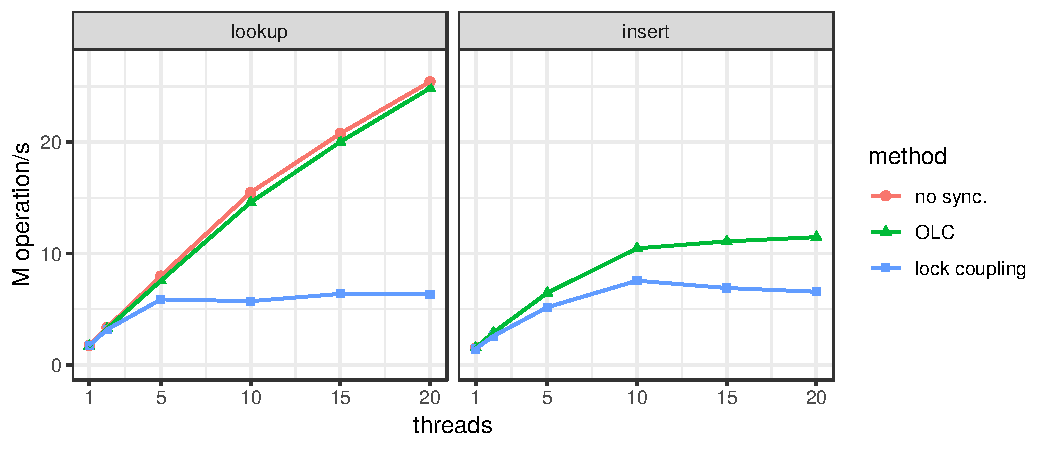
\includegraphics[width=\linewidth]{scale.pdf}
  \vspace{0.2cm}
  \caption{Scalability on 10-core system for B-tree operations (100M values).}
  \label{fig:scale}
\end{figure}

As Figure~\ref{fig:scale} shows, the results change dramatically once we use multiple threads.
For lookup, the scalability of OLC is near-linear up to 20 threads, even though the system has only 10 ``real cores''.
The OLC scalability for insert is also respectable (though not quite as linear because multi-threaded insertion approaches the memory bandwidth of our processor).
The figure also shows that the results of traditional lock coupling with read/write locks are significantly worse than OLC.
With 20 threads, lookup with OLC is 3.9$\times$ faster than traditional lock coupling.

\section{Summary}\label{sec:conc}

Optimistic Lock Coupling (OLC) is an effective synchronization method that combines the simplicity of traditional lock coupling with the superior scalability of lock-free approaches.
OLC is widely applicable and has already been successfully used to synchronize several data structures, including B-trees, binary search trees, and different trie variants.
These features make it highly attractive for modern database systems as well as performance-critical systems software in general.

\begin{thebibliography}{10}

\bibitem{DBLP:conf/spaa/BalmauGHZ16}
O.~Balmau, R.~Guerraoui, M.~Herlihy, and I.~Zablotchi.
\newblock Fast and robust memory reclamation for concurrent data structures.
\newblock In {\em SPAA}, 2016.

\bibitem{DBLP:journals/acta/BayerS77}
R.~Bayer and M.~Schkolnick.
\newblock Concurrency of operations on {B}-trees.
\newblock {\em Acta Informatica}, 9, 1977.

\bibitem{hot}
R.~Binna, E.~Zangerle, M.~Pichl, G.~Specht, and V.~Leis.
\newblock {HOT}: A height optimized trie index for main-memory database
  systems.
\newblock In {\em SIGMOD}, 2018.

\bibitem{DBLP:conf/ppopp/BronsonCCO10}
N.~G. Bronson, J.~Casper, H.~Chafi, and K.~Olukotun.
\newblock A practical concurrent binary search tree.
\newblock In {\em PPOPP}, 2010.

\bibitem{DBLP:conf/vldb/ChaHKK01}
S.~K. Cha, S.~Hwang, K.~Kim, and K.~Kwon.
\newblock Cache-conscious concurrency control of main-memory indexes on
  shared-memory multiprocessor systems.
\newblock In {\em VLDB}, 2001.

\bibitem{intel}
I.~Cutress.
\newblock {Intel} goes for 48-cores: {Cascade-AP} with multi-chip package
  coming soon.
\newblock
  \url{https://www.anandtech.com/show/13535/intel-goes-for-48cores-cascade-ap},
  2018 (accessed January, 2019).

\bibitem{DBLP:conf/cidr/FaleiroA17}
J.~M. Faleiro and D.~J. Abadi.
\newblock Latch-free synchronization in database systems: Silver bullet or
  fool's gold?
\newblock In {\em CIDR}, 2017.

\bibitem{DBLP:journals/ftdb/Graefe11}
G.~Graefe.
\newblock Modern {B}-tree techniques.
\newblock {\em Foundations and Trends in Databases}, 3(4), 2011.

\bibitem{DBLP:conf/hpca/KarnagelDRLLSL14}
T.~Karnagel, R.~Dementiev, R.~Rajwar, K.~Lai, T.~Legler, B.~Schlegel, and
  W.~Lehner.
\newblock Improving in-memory database index performance with
  {Intel}\({}^{\mbox{{\textregistered}}}\) transactional synchronization
  extensions.
\newblock In {\em HPCA}, 2014.

\bibitem{DBLP:journals/tods/LehmanY81}
P.~L. Lehman and S.~B. Yao.
\newblock Efficient locking for concurrent operations on {B}-trees.
\newblock {\em {ACM} Trans. Database Syst.}, 6(4), 1981.

\bibitem{leanstore}
V.~Leis, M.~Haubenschild, A.~Kemper, and T.~Neumann.
\newblock Leanstore: In-memory data management beyond main memory.
\newblock In {\em ICDE}, 2018.

\bibitem{art}
V.~Leis, A.~Kemper, and T.~Neumann.
\newblock The adaptive radix tree: {ARTful} indexing for main-memory databases.
\newblock In {\em ICDE}, 2013.

\bibitem{htmtkde}
V.~Leis, A.~Kemper, and T.~Neumann.
\newblock Scaling {HTM}-supported database transactions to many cores.
\newblock {\em {IEEE} Trans. Knowl. Data Eng.}, 28(2), 2016.

\bibitem{artsync}
V.~Leis, F.~Scheibner, A.~Kemper, and T.~Neumann.
\newblock The {ART} of practical synchronization.
\newblock In {\em DaMoN}, 2016.

\bibitem{DBLP:conf/icde/LevandoskiLS13a}
J.~J. Levandoski, D.~B. Lomet, and S.~Sengupta.
\newblock The {Bw}-tree: A {B}-tree for new hardware platforms.
\newblock In {\em ICDE}, 2013.

\bibitem{DBLP:journals/pvldb/MakreshanskiLS15}
D.~Makreshanski, J.~J. Levandoski, and R.~Stutsman.
\newblock To lock, swap, or elide: On the interplay of hardware transactional
  memory and lock-free indexing.
\newblock {\em {PVLDB}}, 8(11), 2015.

\bibitem{DBLP:dblp_conf/eurosys/MaoKM12}
Y.~Mao, E.~Kohler, and R.~T. Morris.
\newblock Cache craftiness for fast multicore key-value storage.
\newblock In {\em EuroSys}, 2012.

\bibitem{DBLP:journals/tpds/Michael04}
M.~M. Michael.
\newblock Hazard pointers: Safe memory reclamation for lock-free objects.
\newblock {\em {IEEE} Trans. Parallel Distrib. Syst.}, 15(6), 2004.

\bibitem{DBLP:journals/jacm/ShalevS06}
O.~Shalev and N.~Shavit.
\newblock Split-ordered lists: Lock-free extensible hash tables.
\newblock {\em J. {ACM}}, 53(3), 2006.

\bibitem{amd}
A.~Shilov.
\newblock {AMD} previews {EPYC} ‘{Rome}’ processor: Up to 64 {Zen} 2 cores.
\newblock
  \url{https://www.anandtech.com/show/13561/amd-previews-epyc-rome-processor-up-to-64-zen-2-cores},
  2018 (accessed January, 2019).

\bibitem{DBLP:conf/sosp/TuZKLM13}
S.~Tu, W.~Zheng, E.~Kohler, B.~Liskov, and S.~Madden.
\newblock Speedy transactions in multicore in-memory databases.
\newblock In {\em SOSP}, 2013.

\bibitem{buzzword}
Z.~Wang, A.~Pavlo, H.~Lim, V.~Leis, H.~Zhang, M.~Kaminsky, and D.~Andersen.
\newblock Building a {Bw}-tree takes more than just buzz words.
\newblock In {\em SIGMOD}, 2018.

\end{thebibliography}


%\bibliographystyle{abbrv}
%\bibliography{main}

\end{document}

\end{article}









\iffalse

\begin{article}
{{ProvDB:} Provenance-enabled Lifecycle Management of Collaborative Data Analysis Workflows}
{Hui Miao, Amol Deshpande}
\graphicspath{{submissions/ProvDB/figs/}}
\pdfminorversion=5
\documentclass[11pt]{article}
\usepackage{deauthor,times,graphicx,caption,microtype}
\usepackage{hyperref}
\usepackage{listings}
\usepackage{booktabs}

\begin{document}

\title{Optimistic Lock Coupling: A Scalable and Efficient General-Purpose Synchronization Method}

\author{Viktor Leis, Michael Haubenschild\raisebox{0.9ex}{$\ast$}, Thomas Neumann\\ Technische Universit{\"a}t M{\"u}nchen \hspace{0.7cm} Tableau Software\raisebox{0.9ex}{$\ast$} \\ {\{leis,neumann\}{@}in.tum.de} \hspace{0.7cm} {mhaubenschild{@}tableau.com\raisebox{0.9ex}{$\ast$}}}

\maketitle

\begin{abstract}
As the number of cores on commodity processors continues to increase, scalability becomes more and more crucial for overall performance.
Scalable and efficient concurrent data structures are particularly important, as these are often the building blocks of parallel algorithms.
Unfortunately, traditional synchronization techniques based on fine-grained locking have been shown to be unscalable on modern multi-core CPUs.
Lock-free data structures, on the other hand, are extremely difficult to design and often incur significant overhead.

In this work, we make the case for Optimistic Lock Coupling as a practical alternative to both traditional locking and the lock-free approach.
We show that Optimistic Lock Coupling is highly scalable and almost as simple to implement as traditional lock coupling.
Another important advantage is that it is easily applicable to most tree-like data structures.
We therefore argue that Optimistic Lock Coupling, rather than a complex and error-prone custom synchronization protocol, should be the default choice for performance-critical data structures.
\end{abstract}

\section{Introduction}

% more and more cores
Today, Intel's commodity server processors have up to 28 cores and its upcoming microarchitecture will have up to 48 cores per socket~\cite{intel}.
Similarly, AMD currently stands at 32 cores and this number is expected to double in the next generation~\cite{amd}.
Since both platforms support simultaneous multithreading (also known as hyperthreading), affordable commodity servers (with up to two sockets) will soon routinely have between 100 and 200 hardware threads.

% data structure scalability is important
With such a high degree of hardware parallelism, efficient data processing crucially depends on how well concurrent data structures scale.
Internally, database systems use a plethora of data structures like table heaps, internal work queues, and, most importantly, index structures.
Any of these can easily become a scalability (and therefore overall performance) bottleneck on many-core CPUs.

% traditional synchronization: fine-grained locks, slow, cache invalidation
Traditionally, database systems synchronize internal data structures using fine-grained reader/writer locks\footnote{In this work, we focus on data structure synchronization rather than high-level transaction semantics and therefore use the term {\em lock} for what would typically be called {\em latch} in the database literature. We thus follow common computer science (rather than database) terminology.}.
Unfortunately, while fine-grained locking makes lock contention unlikely, it still results in bad scalability because lock acquisition and release require writing to shared memory.
Due to the way cache coherency is implemented on modern multi-core CPUs, these writes cause additional cache misses\footnote{The cache coherency protocol ensures that all copies of a cache line on other cores are invalidated before the write can proceed.} and the cache line containing the lock's internal data becomes a point of physical contention.
As a result, any frequently-accessed lock (e.g., the lock of the root node of a B-tree) severely limits scalability.

% lock-free bw-tree: no more latches, but indirections, extremely complex
Lock-free data structures like the Bw-tree~\cite{DBLP:conf/icde/LevandoskiLS13a} (a lock-free B-tree variant) or the Split-Ordered List~\cite{DBLP:journals/jacm/ShalevS06} (a lock-free hash table) do not acquire any locks and therefore generally scale much better than locking-based approaches (in particular for read-mostly workloads).
However, lock-free synchronization has other downsides:
First, it is very difficult and results in extremely complex and error-prone code (when compared to locking).
Second, because the functionality of atomic primitives provided by the hardware (e.g., atomically compare-and-swap 8 bytes) is limited, complex operations require additional indirections within the data structure.
For example, the Bw-tree requires an indirection table and the Split-Ordered List requires ``dummy nodes'', resulting in overhead due to additional cache misses.

% OLC for the win
In this paper we make the case for {\em Optimistic Lock Coupling (OLC)}, a synchronization method that combines some of the best properties of lock-based and lock-free synchronization.
OLC utilizes a special lock type that can be used in two modes:
The first mode is similar to a traditional mutex and excludes other threads by physically acquiring the underlying lock.
In the second mode, reads can proceed optimistically by validating a version counter that is embedded in the lock (similar to optimistic concurrency control).
The first mode is typically used by writers and the second mode by readers.
Besides this special lock type, OLC is based on the observation that optimistic lock validations can be interleaved/coupled---similar to the pair-wise interleaved lock acquisition of traditional lock coupling.
Hence, the name Optimistic Lock Coupling.

OLC has a number of desirable features:
\begin{itemize}
\item By reducing the number of writes to shared memory locations and thereby avoiding cache invalidations, it {\bf scales well} for most workloads.
\item In comparison to unsynchronized code, it requires few additional CPU instructions making it {\bf efficient}.
\item OLC is {\bf widely applicable} to different data structures. It has already been successfully used for synchronizing binary search trees~\cite{DBLP:conf/ppopp/BronsonCCO10}, tries~\cite{artsync}, trie/B-tree hybrids~\cite{DBLP:dblp_conf/eurosys/MaoKM12}, and B-trees~\cite{buzzword}.
\item In comparison to the lock-free paradigm, it is also {\bf easy to use} and requires few modifications to existing, single-threaded data structures.
\end{itemize}
Despite these positive features and its simplicity, OLC is not yet widely known.
The goal of this paper is therefore to popularize this simple idea and to make a case for it.
We argue that OLC deserves to be widely known.
It is a good default synchronization paradigm---more complex, data structure-specific protocols are seldom beneficial.

The rest of the paper is organized as follows.
Section~\ref{sec:related} discusses related work, tracing the history of OLC and its underlying ideas in the literature.
The core of the paper is Section~\ref{sec:olc}, which describes the ideas behind OLC and how it can be used to synchronize complex data structures.
In Section~\ref{sec:evaluation} we experimentally show that OLC has low overhead and scales well when used to synchronize an in-memory B-tree.
We summarize the paper in Section~\ref{sec:conc}.

\newpage
\section{Related Work}\label{sec:related}

Lock coupling has been proposed as a method for allowing concurrent operations on B-trees in 1977~\cite{DBLP:journals/acta/BayerS77}.
This traditional and still widely-used method, described in detail in Graefe's B-tree survey~\cite{DBLP:journals/ftdb/Graefe11}, is also called ``latch coupling'', ``hand-over-hand locking'', and ``crabbing''.
Because at most two locks are held at-a-time during tree traversal, this technique seemingly allows for a high degree of parallelism---in particular if read/write locks are used to enable inner nodes to be locked in shared mode.
However, as we show in Section~\ref{sec:evaluation}, on modern hardware lock acquisition (even in shared mode) results in suboptimal scalability.

An early alternative from 1981 is a B-tree variant called B-link tree~\cite{DBLP:journals/tods/LehmanY81}, which only holds a single lock at a time.
It is based on the observation that between the release of the parent lock and the acquisition of the child lock, the only ``dangerous'' thing that could have happened is the split of a child node (assuming one does not implement merge operations).
Thus, when a split happens, the key being searched might end up on a neighboring node to the right of the current child node.
A B-link tree traversal therefore detects this condition and, if needed, transparently proceeds to the neighboring node.
Releasing the parent lock early is highly beneficial when the child node needs to be fetched from disk.
For in-memory workloads, however, the B-link tree has the same scalability issues as lock coupling (it acquires just as many locks).

The next major advance, Optimistic Latch-Free Index Traversal (OLFIT)~\cite{DBLP:conf/vldb/ChaHKK01}, was proposed in 2001.
OLFIT introduced the idea of a combined lock/update counter, which we call {\em optimistic lock}. % , for lack of a better name,
Based on these per-node optimistic locks and the synchronization protocol of the B-link tree, OLFIT finally achieves good scalability on parallel processors.
The OLFIT protocol is fairly complex, as it requires both the non-trivial B-link protocol and optimistic locks.
Furthermore, like the B-link tree protocol, it does not support merging nodes, and is specific to B-trees (cannot easily be applied to other data structures).

In the following two decades, the growth of main-memory capacity led to much research into other data structures besides the venerable B-tree.
Particularly relevant for our discussion is Bronson et al.'s~\cite{DBLP:conf/ppopp/BronsonCCO10} concurrent binary search tree, which is based on optimistic version validation and has a sophisticated, data structure-specific synchronization protocol.
To the best of our knowledge, this 2010 paper is the first that, as part of its protocol, interleaves version validation across nodes---rather than validating each node separately like OLFIT.
In that paper, this idea is called ``hand-over-hand, optimistic validation'', while we prefer the term Optimistic Lock Coupling to highlight the close resemblance to traditional lock coupling.
Similarly, Mao et al.'s~\cite{DBLP:dblp_conf/eurosys/MaoKM12} Masstree (a concurrent hybrid trie/B-tree) is also based on the same ideas, but again uses them as part of a more complex protocol.

The Adaptive Radix Tree (ART)~\cite{art} is another recent in-memory data structure, which we proposed in 2013.
In contrast to the two data structures just mentioned, it was originally designed with single-threaded performance in mind without supporting concurrency.
To add support for concurrency, we initially started designing a custom protocol called Read-Optimized Write Exclusion (ROWEX)~\cite{artsync}, which turned out to be non-trivial and requires modifications of the underlying data structure\footnote{Note that ROWEX is already easier to apply to existing data structures than the lock-free approach. The difficulty depends on the data structure. Applying ROWEX is hard for B-trees with sorted keys and fairly easy for copy-on-write data structures like the Height Optimized Trie~\cite{hot}---with ART being somewhere in the middle.}.
However, fairly late in the project, we also realized, that OLC {\em alone} (rather than as part of a more complex protocol) is sufficient to synchronize ART.
No other changes to the data structure were necessary.
Both approaches were published and experimentally evaluated in a followup paper~\cite{artsync}, which shows that, despite its simplicity, OLC is efficient, scalable, and generally outperforms ROWEX.

Similar results were recently published regarding B-trees~\cite{buzzword}.
In this experimental study a simple OLC-based synchronization outperformed the Bw-tree~\cite{DBLP:conf/icde/LevandoskiLS13a}, a complex lock-free synchronization approach.
Another recent paper shows that for write-intensive workloads, locking often performs better than lock-free synchronization~\cite{DBLP:conf/cidr/FaleiroA17}.
These experiences indicate that OLC is a general-purpose synchronization paradigm and motivate the current paper.

%foster b-tree\cite{DBLP:journals/tods/GraefeKK12}
%Shasha theory~\cite{DBLP:journals/tods/ShashaG88}

\section{Optimistic Lock Coupling}\label{sec:olc}

% locks suck
The standard technique for inter-thread synchronization is mutual exclusion using fine-grained locks.
In a B-tree, for example, every node usually has its own associated lock, which is acquired before accessing that node.
The problem of locking on modern multi- and many-core processors is that lock acquisition and release require writing to the shared memory location that implements the lock.
This write causes exclusive ownership of the underlying cache line and invalidates copies of it on all other processor cores.
For hierarchical, tree-like data structures, the lock of the root node becomes a point of physical contention---even in read-only workloads and even when read/write locks are used.
Depending on the specific data structure, number of cores, cache coherency protocol implementation, cache topology, whether Non-Uniform Memory Access (NUMA) is used, locking can even result in multi-threaded performance that is worse than single-threaded execution.

% in b-trees this happens very much
The inherent pessimism of locking is particularly unfortunate for B-trees:
Despite the fact that logical modifications of the root node are very infrequent, every B-tree operation must lock the root node during tree traversal\footnote{To a lesser extent this obviously applies to all inner nodes, not just the root.}.
Even the vast majority of update operations (with the exception of splits and merges), only modify a single leaf node.
These observations indicate that a more optimistic approach, which does not require locking inner nodes, would be very beneficial for B-trees.

\subsection{Optimistic Locks}

% optimism to the rescue
As the name indicates, optimistic locks try to solve the scalability issues of traditional locks using an optimistic approach.
Instead of always physically acquiring locks, even for nodes that are unlikely to be modified simultaneously, after-the-fact validation is used to detect conflicts.
This is done by augmenting each lock with a version/update counter that is incremented on every modification.
Using this version counter, readers can optimistically proceed before validating that the version did not change to ensure that the read was safe.
If validation fails, the operation is restarted.

% details on opt locks
Using optimistic locks, a read-only node access (i.e., the majority of all operations in a B-tree) does not acquire the lock and does not increment the version counter.
Instead, it performs the following steps:
\begin{enumerate}
\item read lock version (restart if lock is not free)
\item access node
\item read the version again and validate that it has not changed in the meantime
\end{enumerate}
If the last step (the validation) fails, the operation has to be restarted.
Write operations, on the other hand, are more similar to traditional locking:
\begin{enumerate}
\item acquire lock (wait if necessary)
\item access/write to node
\item increment version and unlock node
\end{enumerate}
Writes can therefore protect a node from other writes.

% similar to locks
As we observed in an earlier paper~\cite{artsync}, because of similar semantics, optimistic locks can be hidden behind an API very similar to traditional read/write locks.
Both approaches have an exclusive lock mode, and acquiring a traditional lock in shared mode is analogous to optimistic version validation.
Furthermore, like with some implementations of traditional read/write locks, optimistic locks allow upgrading a shared lock to an exclusive lock.
Lock upgrades are, for example, used to avoid most B-tree update operations from having to lock inner nodes.
In our experience, the close resemblance of optimistic and traditional locks simplifies the reasoning about optimistic locks;
one can apply similar thinking as in traditional lock-based protocols.

\subsection{Lock Coupling with Optimistic Locks}

\begin{figure}
  \centering
  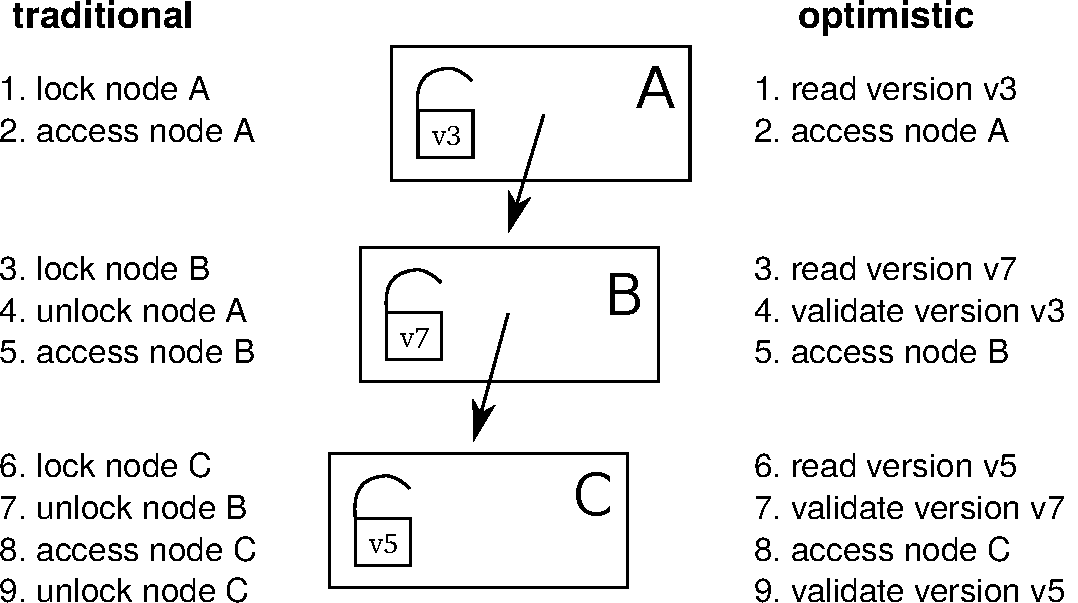
\includegraphics[width=0.65\linewidth]{olcall.pdf}
  \vspace{0.2cm}
  \caption{Comparison of a lookup operation in a 3-level tree using traditional lock coupling (left-hand side) vs.~optimistic lock coupling (right-hand side).}
  \label{fig:olc}
\end{figure}

The traditional and most common lock-based synchronization protocol for B-trees is lock coupling, which interleaves lock acquisitions while holding at most two locks at a time.
If, as we observed earlier, optimistic locks have similar semantics as traditional locks, it is natural to ask whether lock coupling can be combined with optimistic locks.
And indeed the answer is yes: One can almost mechanically translate traditional lock coupling code to optimistic lock coupling code.
This is illustrated in Figure~\ref{fig:olc}, which compares the traversal in a tree of height 3 using traditional and optimistic locks.
As the figure shows, the main difference is that locking is translated to reading the version and that unlocking becomes validation of the previously read version.
This simple change provides efficient lock-free tree traversal without the need to design a complex synchronization protocol.

It is important to emphasize the conceptual simplicity of OLC in comparison to data structures that use custom protocols like the Bw-tree~\cite{DBLP:conf/icde/LevandoskiLS13a}.
To implement lock-free access, the Bw-tree requires an indirection table, delta nodes, complex splitting and merging logic, retry logic, etc.
OLC, on the other hand, can directly be applied to B-trees mostly by adding the appropriate optimistic locking code and without modifying the node layout itself.
Therefore, OpenBw-Tree, an open source implementation of the Bw-tree, requires an order of magnitude more code than a B-tree based on OLC\footnote{Both implementations are available on GitHub: \url{https://github.com/wangziqi2016/index-microbench}}.
Given how difficult it is to develop, validate, and debug lock-free code, simplicity is obviously a major advantage.

\subsection{Correctness Aspects}

\begin{figure}
  % \centering
  %[basicstyle=\normalsize\ttfamily,showstringspaces=false,columns=fullflexible,breaklines=false,breakatwhitespace=true,numbers=none,numberstyle=\small,style=C,keepspaces=true]
\begin{lstlisting}[basicstyle=\ttfamily,language=C++,numbers=left,numberstyle=\small]
std::atomic<BTreeNode*> root;

// search for key in B+tree, returns payload in resultOut
bool lookup(Key key, Value& resultOut) {
   BTreeNode* node = root.load();
   uint64_t nodeVersion = node->readLockOrRestart();
   if (node != root.load()) // make sure the root is still the root
      restart();

   BTreeInner<Key>* parent = nullptr;
   uint64_t parentVersion = 0;

   while (node->isInner()) {
      auto inner = (BTreeInner*)node;

      // unlock parent and make current node the parent
      if (parent)
         parent->readUnlockOrRestart(parentVersion);
      parent = inner;
      parentVersion = nodeVersion;

      // search for next node
      node = inner->findChild(key);
      // validate 'inner' to ensure that 'node' pointer is valid
      inner->checkOrRestart(nodeVersion);
      // now it safe to dereference 'node' pointer (read its version)
      nodeVersion = node->readLockOrRestart();
   }

   // search in leaf and retrieve payload
   auto leaf = (BTreeLeaf*)node;
   bool success = leaf->findValue(key, resultOut);

   // unlock everything
   if (parent)
      parent->readUnlockOrRestart(parentVersion);
   node->readUnlockOrRestart(nodeVersion);

   return success;
}
\end{lstlisting}
  \vspace{0.2cm}
  \caption{B-tree lookup code using OLC. For simplicity, the restart logic is not shown.}
  \label{fig:lookup}
\end{figure}

So far, we have introduced the high-level ideas behind OLC and have stressed its similarity to traditional lock coupling.
Let us now discuss some cases where the close similarity between lock coupling and OLC breaks down.
To make this more concrete, we show the B-tree lookup code in Figure~\ref{fig:lookup}.
In the code, \texttt{readLockOrRestart} reads the lock version and \texttt{readUnlockOrRestart} validates that the read was correct.

One issue with OLC is that any pointer speculatively read from a node may point to invalid memory (if that node is modified concurrently).
Dereferencing such a pointer (e.g., to read its optimistic lock), may cause a segmentation fault or undefined behavior.
In the code shown in Figure~\ref{fig:lookup}, this problem is prevented by the extra check in line 25, which ensures that the read from the node containing the pointer was correct.
Without this additional validation, the code would in line 27 dereference the pointer speculatively read in line 23.
Note that the implementation of \texttt{checkOrRestart} is actually identical to \texttt{readUnlockOrRestart}.
We chose to give it a different name to highlight the fact that this extra check would not be necessary with read/write locks.

Another potential issue with optimistic locks is code that does not terminate.
Code that speculatively accesses a node, like an intra-node binary search, should be written in a way such that it always terminates---even in the presence of concurrent writes.
Otherwise, the validation code that detects the concurrent write will never run.
The binary search of a B-tree, for example, needs to be written in such a way that each comparison makes progress.
For some data structures that do not require loops in the traversal code (like ART) termination is trivially true.

\subsection{Implementation Details}

% implementation, efficiency
To implement an optimistic lock, one can combine the lock and the version counter into a single 64-bit\footnote{Even after subtracting one bit for the lock status, a back-of-the-envelope calculation can show that 63 bits are large enough to never overflow in practice.} word~\cite{artsync}.
A typical read operation will therefore merely consist of reading this version counter atomically.
In C++11 this can be implemented using the \texttt{std::atomic} type.

On x86, atomic reads are cheap because of x86's strong memory order guarantees.
No memory fences are required for sequentially-consistent loads, which are translated (by both GCC and clang) into standard \texttt{MOV} instructions.
Hence, the only effect of \texttt{std::atomic} for loads is preventing instruction re-ordering.
This makes version access and validation cheap.
Acquiring and releasing an optimistic lock in exclusive mode has comparable cost to a traditional lock:
A fairly expensive sequentially-consistent store is needed for acquiring a lock, while a standard \texttt{MOV} suffices for releasing it.
A simple sinlock-based implementation of optimistic locks can be found in the appendix of an earlier paper~\cite{artsync}.

OLC code must be able to handle restarts since validation or lock upgrade can fail due to concurrent writers.
Restarts can easily be implemented by wrapping the data structure operation in a loop (for simplicity not shown in Figure~\ref{fig:lookup}).
Such a loop also enables limiting the number of optimistic retry operations and falling back to pessimistic locking in cases of very heavy contention.
The ability to fall back to traditional locking is a major advantage of OLC in terms of robustness over lock-free approaches, which do not have this option.

In addition to the optimistic shared mode and the exclusive mode, optimistic locks also support a ``shared pessimistic'' mode, which physically acquires the lock in shared mode (allowing multiple concurrent readers but no writers).
This mode is useful for table (or range) scans that touch many tuples on a leaf page (which would otherwise easily abort).
Finally, let us mention that large range scans and table scans, should be broken up into several per-node traversals as is done in the LeanStore~\cite{leanstore} system.

Like all lock-free data structures, but unlike traditional locking and Hardware Transactional Memory~\cite{DBLP:conf/hpca/KarnagelDRLLSL14,DBLP:journals/pvldb/MakreshanskiLS15,htmtkde}, OLC requires care when deleting (and reusing) nodes.
The reason is that a deleting thread can never be sure that a node can be reclaimed because other threads might still be optimistically reading from that node.
Therefore, standard solutions like epoch-based reclamation~\cite{DBLP:conf/sosp/TuZKLM13}, hazard pointers~\cite{DBLP:journals/tpds/Michael04}, or optimized hazard pointers~\cite{DBLP:conf/spaa/BalmauGHZ16} need to be used.
These memory reclamation techniques are, however, largely orthogonal to the synchronization protocol itself.

%-lock-free is not a strong guarantee

\newpage
\section{Evaluation}\label{sec:evaluation}

Let us now experimentally evaluate the overhead and scalability of OLC.
For the experiments, we use an in-memory B+tree implemented in C++11 using templates, which is configured to use nodes of 4096 bytes, random 8 byte keys, and 8 byte payloads.
Based on this B-tree, we compare the following synchronization approaches:
\begin{itemize}
\item an OLC implementation\footnote{An almost identical OLC implementation is available on github: \url{https://github.com/wangziqi2016/index-microbench/tree/master/BTreeOLC}}
\item a variant based on traditional lock coupling and read/write locks
\item the unsynchronized B-tree, which obviously is only correct for read-only workloads but allows measuring the overhead of synchronization
\end{itemize}
Note that earlier work has compared the OLC implementation with a Bw-tree implementation~\cite{buzzword} and other state-of-the-art in-memory index structures.

We use a Haswell EP system with an Intel Xeon E5-2687W v3 CPU, which has 10 cores (20 ``Hyper-Threads'') and 25~MB of L3 cache.
The system is running Ubuntu 18.10 and we use GCC 8.2.0 to compile our code.
The CPU counters are obtained using the Linux perf API\footnote{We use the following convenience wrapper: \url{https://github.com/viktorleis/perfevent}}.

\begin{table}
  \caption{Performance and CPU counters for lookup and insert operations in a B-tree with 100M keys. We perform 100M operations and normalize the CPU counters by that number.}
  \label{tab:overhead}
  \centering
  \begin{tabular}{lrrrrrrr}\toprule
                    &         &        &        & instruc-  & L1     & L3     & branch \\
                    & threads & M op/s & cycles & tions & misses & misses & misses \\\midrule
lookup (no sync.)   & 1       & 1.72   & 2028   & 283     & 39.1   & 14.9   & 16.1   \\
lookup (OLC)        & 1       & 1.65   & 2107   & 370     & 43.9   & 15.1   & 16.7   \\
lookup (lock coup.) & 1       & 1.72   & 2078   & 365     & 42.3   & 16.9   & 15.7   \\\midrule
insert (no sync.)   & 1       & 1.51   & 2286   & 530     & 59.8   & 31.1   & 17.3   \\
insert (OLC)        & 1       & 1.50   & 2303   & 629     & 61.2   & 31.1   & 16.5   \\
insert (lock coup.) & 1       & 1.41   & 2473   & 644     & 61.0   & 31.0   & 17.2   \\\midrule
lookup (no sync.)   & 10      & 15.48  & 2058   & 283     & 38.6   & 15.5   & 16.0   \\
lookup (OLC)        & 10      & 14.60  & 2187   & 370     & 43.8   & 15.8   & 16.8   \\
lookup (lock coup.) & 10      & 5.71   & 5591   & 379     & 54.2   & 17.0   & 14.8   \\\midrule
insert (no sync.)   & 10      & -      & -      & -       & -      & -      & -      \\
insert (OLC)        & 10      & 10.46  & 2940   & 656     & 62.0   & 32.5   & 16.8   \\
insert (lock coup.) & 10      & 7.55   & 4161   & 667     & 75.0   & 28.6   & 16.2   \\
    \bottomrule
\end{tabular}
\end{table}

Table~\ref{tab:overhead} compares the performance and CPU counters for lookup and insert operations in a B-tree with 100M keys.
With {\em single-threaded} execution, we observe that all three approaches have very similar performance.
Adding traditional or optimistic locks to unsynchronized B-tree code results in up to 30\% of additional instructions without affecting single-threaded performance much.

\begin{figure}
  \centering
  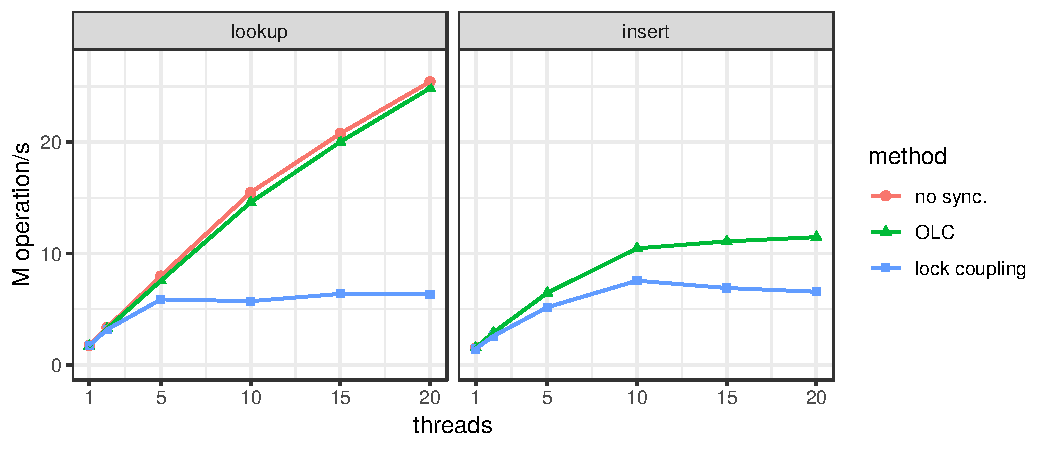
\includegraphics[width=\linewidth]{scale.pdf}
  \vspace{0.2cm}
  \caption{Scalability on 10-core system for B-tree operations (100M values).}
  \label{fig:scale}
\end{figure}

As Figure~\ref{fig:scale} shows, the results change dramatically once we use multiple threads.
For lookup, the scalability of OLC is near-linear up to 20 threads, even though the system has only 10 ``real cores''.
The OLC scalability for insert is also respectable (though not quite as linear because multi-threaded insertion approaches the memory bandwidth of our processor).
The figure also shows that the results of traditional lock coupling with read/write locks are significantly worse than OLC.
With 20 threads, lookup with OLC is 3.9$\times$ faster than traditional lock coupling.

\section{Summary}\label{sec:conc}

Optimistic Lock Coupling (OLC) is an effective synchronization method that combines the simplicity of traditional lock coupling with the superior scalability of lock-free approaches.
OLC is widely applicable and has already been successfully used to synchronize several data structures, including B-trees, binary search trees, and different trie variants.
These features make it highly attractive for modern database systems as well as performance-critical systems software in general.

\begin{thebibliography}{10}

\bibitem{DBLP:conf/spaa/BalmauGHZ16}
O.~Balmau, R.~Guerraoui, M.~Herlihy, and I.~Zablotchi.
\newblock Fast and robust memory reclamation for concurrent data structures.
\newblock In {\em SPAA}, 2016.

\bibitem{DBLP:journals/acta/BayerS77}
R.~Bayer and M.~Schkolnick.
\newblock Concurrency of operations on {B}-trees.
\newblock {\em Acta Informatica}, 9, 1977.

\bibitem{hot}
R.~Binna, E.~Zangerle, M.~Pichl, G.~Specht, and V.~Leis.
\newblock {HOT}: A height optimized trie index for main-memory database
  systems.
\newblock In {\em SIGMOD}, 2018.

\bibitem{DBLP:conf/ppopp/BronsonCCO10}
N.~G. Bronson, J.~Casper, H.~Chafi, and K.~Olukotun.
\newblock A practical concurrent binary search tree.
\newblock In {\em PPOPP}, 2010.

\bibitem{DBLP:conf/vldb/ChaHKK01}
S.~K. Cha, S.~Hwang, K.~Kim, and K.~Kwon.
\newblock Cache-conscious concurrency control of main-memory indexes on
  shared-memory multiprocessor systems.
\newblock In {\em VLDB}, 2001.

\bibitem{intel}
I.~Cutress.
\newblock {Intel} goes for 48-cores: {Cascade-AP} with multi-chip package
  coming soon.
\newblock
  \url{https://www.anandtech.com/show/13535/intel-goes-for-48cores-cascade-ap},
  2018 (accessed January, 2019).

\bibitem{DBLP:conf/cidr/FaleiroA17}
J.~M. Faleiro and D.~J. Abadi.
\newblock Latch-free synchronization in database systems: Silver bullet or
  fool's gold?
\newblock In {\em CIDR}, 2017.

\bibitem{DBLP:journals/ftdb/Graefe11}
G.~Graefe.
\newblock Modern {B}-tree techniques.
\newblock {\em Foundations and Trends in Databases}, 3(4), 2011.

\bibitem{DBLP:conf/hpca/KarnagelDRLLSL14}
T.~Karnagel, R.~Dementiev, R.~Rajwar, K.~Lai, T.~Legler, B.~Schlegel, and
  W.~Lehner.
\newblock Improving in-memory database index performance with
  {Intel}\({}^{\mbox{{\textregistered}}}\) transactional synchronization
  extensions.
\newblock In {\em HPCA}, 2014.

\bibitem{DBLP:journals/tods/LehmanY81}
P.~L. Lehman and S.~B. Yao.
\newblock Efficient locking for concurrent operations on {B}-trees.
\newblock {\em {ACM} Trans. Database Syst.}, 6(4), 1981.

\bibitem{leanstore}
V.~Leis, M.~Haubenschild, A.~Kemper, and T.~Neumann.
\newblock Leanstore: In-memory data management beyond main memory.
\newblock In {\em ICDE}, 2018.

\bibitem{art}
V.~Leis, A.~Kemper, and T.~Neumann.
\newblock The adaptive radix tree: {ARTful} indexing for main-memory databases.
\newblock In {\em ICDE}, 2013.

\bibitem{htmtkde}
V.~Leis, A.~Kemper, and T.~Neumann.
\newblock Scaling {HTM}-supported database transactions to many cores.
\newblock {\em {IEEE} Trans. Knowl. Data Eng.}, 28(2), 2016.

\bibitem{artsync}
V.~Leis, F.~Scheibner, A.~Kemper, and T.~Neumann.
\newblock The {ART} of practical synchronization.
\newblock In {\em DaMoN}, 2016.

\bibitem{DBLP:conf/icde/LevandoskiLS13a}
J.~J. Levandoski, D.~B. Lomet, and S.~Sengupta.
\newblock The {Bw}-tree: A {B}-tree for new hardware platforms.
\newblock In {\em ICDE}, 2013.

\bibitem{DBLP:journals/pvldb/MakreshanskiLS15}
D.~Makreshanski, J.~J. Levandoski, and R.~Stutsman.
\newblock To lock, swap, or elide: On the interplay of hardware transactional
  memory and lock-free indexing.
\newblock {\em {PVLDB}}, 8(11), 2015.

\bibitem{DBLP:dblp_conf/eurosys/MaoKM12}
Y.~Mao, E.~Kohler, and R.~T. Morris.
\newblock Cache craftiness for fast multicore key-value storage.
\newblock In {\em EuroSys}, 2012.

\bibitem{DBLP:journals/tpds/Michael04}
M.~M. Michael.
\newblock Hazard pointers: Safe memory reclamation for lock-free objects.
\newblock {\em {IEEE} Trans. Parallel Distrib. Syst.}, 15(6), 2004.

\bibitem{DBLP:journals/jacm/ShalevS06}
O.~Shalev and N.~Shavit.
\newblock Split-ordered lists: Lock-free extensible hash tables.
\newblock {\em J. {ACM}}, 53(3), 2006.

\bibitem{amd}
A.~Shilov.
\newblock {AMD} previews {EPYC} ‘{Rome}’ processor: Up to 64 {Zen} 2 cores.
\newblock
  \url{https://www.anandtech.com/show/13561/amd-previews-epyc-rome-processor-up-to-64-zen-2-cores},
  2018 (accessed January, 2019).

\bibitem{DBLP:conf/sosp/TuZKLM13}
S.~Tu, W.~Zheng, E.~Kohler, B.~Liskov, and S.~Madden.
\newblock Speedy transactions in multicore in-memory databases.
\newblock In {\em SOSP}, 2013.

\bibitem{buzzword}
Z.~Wang, A.~Pavlo, H.~Lim, V.~Leis, H.~Zhang, M.~Kaminsky, and D.~Andersen.
\newblock Building a {Bw}-tree takes more than just buzz words.
\newblock In {\em SIGMOD}, 2018.

\end{thebibliography}


%\bibliographystyle{abbrv}
%\bibliography{main}

\end{document}

\end{article}


\begin{article}
{Accelerating the Machine Learning Lifecycle with {MLflow}}
{Matei Zaharia, Andrew Chen, Aaron Davidson, Ali Ghodsi, Sue Ann Hong, Andy Konwinski, Siddharth Murching, Tomas Nykodym, Paul Ogilvie, Mani Parkhe, Fen Xie, Corey Zumar}
\graphicspath{{submissions/mlflow/}}
\documentclass[11pt]{article}
%\documentclass[11pt,dvipdfm]{article}

\usepackage{deauthor}
\usepackage{url}            % simple URL typesetting
\usepackage{graphicx}
\usepackage{times}
\usepackage{fancyvrb}
\usepackage{comment}

% \graphicspath{{authorname/}}

\begin{document}

%\title{MLflow: An Open Platform for Machine Learning Experimentation, Reproducibility and Production}
%\title{MLflow: An Open Platform for the End-to-End Machine Learning Lifecycle}
\title{Accelerating the Machine Learning Lifecycle with {MLflow}}

% The \author macro works with any number of authors. There are two
% commands used to separate the names and addresses of multiple
% authors: \And and \AND.
%
% Using \And between authors leaves it to LaTeX to determine where to
% break the lines. Using \AND forces a line break at that point. So,
% if LaTeX puts 3 of 4 authors names on the first line, and the last
% on the second line, try using \AND instead of \And before the third
% author name.

\author{
  \textbf{Matei Zaharia, Andrew Chen, Aaron Davidson, Ali Ghodsi, Sue Ann Hong, Andy Konwinski,}\\
  \textbf{Siddharth Murching, Tomas Nykodym, Paul Ogilvie, Mani Parkhe, Fen Xie, Corey Zumar} \\
  Databricks Inc.\\
  %% examples of more authors
  %% \And
  %% Coauthor \\
  %% Affiliation \\
  %% Address \\
  %% \texttt{email} \\
  %% \AND
  %% Coauthor \\
  %% Affiliation \\
  %% Address \\
  %% \texttt{email} \\
  %% \And
  %% Coauthor \\
  %% Affiliation \\
  %% Address \\
  %% \texttt{email} \\
  %% \And
  %% Coauthor \\
  %% Affiliation \\
  %% Address \\
  %% \texttt{email} \\
}

\maketitle

\begin{abstract}
Machine learning development creates multiple new challenges that are not present in a traditional software development lifecycle.
These include keeping track of the myriad inputs to an ML application (e.g., data versions, code and tuning parameters), reproducing results, and production deployment.
In this paper, we summarize these challenges from our experience with Databricks customers, and describe MLflow, an open source platform we recently launched to streamline the machine learning lifecycle.
MLflow covers three key challenges: experimentation, reproducibility, and model deployment, using generic APIs that work with any ML library, algorithm and programming language.
The project has a rapidly growing open source community, with over 50 contributors since its launch in June 2018.
\end{abstract}

\section{Introduction}

Machine learning development requires solving new problems that are not part of the standard software development lifecycle.
For example, while traditional software has a well-defined set of product features to be built, ML development tends to revolve around \emph{experimentation}: the ML developer will constantly experiment with new datasets, models, software libraries, tuning parameters, etc.~to optimize a business metric such as model accuracy.
Because model performance depends heavily on the input data and training process, \emph{reproducibility} is paramount throughout ML development.
Finally, in order to have business impact, ML applications need to be \emph{deployed} to production, which means both deploying a model in a way that can be used for inference (e.g., REST serving) and deploying scheduled jobs to regularly update the model.
This is especially challenging when deployment requires collaboration with another team, such as application engineers who are not ML experts.

Based on our conversations with dozens of Databricks customers that use machine learning, these lifecycle problems are a major bottleneck in practice.
Although today's ML libraries provide tools for part of the lifecycle, there are no standard systems and interfaces to manage the full process.
For example, TensorFlow offers a training API and a Serving system~\cite{tfx}, but TensorFlow Serving cannot easily be used for models from another ML library, or from an incompatible version of TensorFlow.
In practice, an organization will need to run models from multiple ML libraries, TensorFlow versions, etc., and has to design its own infrastructure for this task.


Faced with these challenges, many organizations try to ``lock down'' the ML development process to obtain reproducibility and deployability.
Some organizations develop internal guidelines for ML development, such as which libraries one can use that the production team will support.
Others develop internal \emph{ML platforms} (e.g., Facebook's FBLearner~\cite{fblearner}, Uber's Michelangelo~\cite{michelangelo} and Google's TFX~\cite{tfx}): APIs that ML developers must use in order to build deployable models.
Unfortunately, both approaches limit ML developers in the algorithms and libraries they can use, decreasing their ability to experiment, and both create substantial engineering work whenever the ML developers want to use new libraries or models.

%Some organizations ask each ML team to manage its own infrastructure, which is expensive.
%Others try to develop shared \emph{ML platforms} that data scientists must use to build their models (e.g., Facebook's FBLearner~\cite{fblearner} and Uber's Michelangelo~\cite{michelangelo}), but this approach also has challenges, because model developers are limited to the algorithms and libraries supported by the platform and cannot easily experiment with others.

In this paper, we summarize our experience with ML lifecycle challenges at Databricks customers and describe MLflow, an open source ML platform we are developing to address these challenges.
MLflow's key principle is an \emph{open interface} design, where data scientists and engineers can bring their own training code, metrics, and inference logic while benefitting from a structured development process.
%MLflow leverages simple, generic interfaces such as Docker containers and REST APIs to achieve this goal.
For example, a ``model'' saved in MLflow can simply be a Python function (and associated library dependencies) that MLflow then knows how to deploy in various environments (e.g., batch or real-time scoring).
Other MLflow abstractions are likewise based on generic interfaces, such as REST APIs and Docker containers.
Compared to existing ML platforms like FBLearner, Michelangelo and TFX, this open interface design gives users flexibility and control while retaining the benefits of lifecycle management.
%Moreover, MLflow's open source nature enables easily sharing ML work across organizations.
The current version of MLflow provides APIs for experiment tracking, reproducible runs and model packaging and deployment, usable in Python, Java and R.
We describe these APIs and some sample MLflow use cases to show how the system can streamline the machine learning lifecycle.

\section{Challenges in Machine Learning Development}

ML faces many of the challenges in traditional software development, such as testing, code review, monitoring, etc.
In other ways, however, ML applications are different from traditional software, and present new problems.

One of the main differences is that the goal in machine learning is to \emph{optimize} a specific metric, such as prediction accuracy, instead of simply meeting a set of functional requirements.
For example, for a retailer, every 1\% improvement in prediction accuracy for a recommendation engine might lead to millions of dollars in revenue, so the ML team working on this engine will continuously want to improve the model.
This means that ML developers wish to continuously experiment with the latest models, software libraries, etc.,~to improve target metrics.
Beyond this difference in objective, ML applications are more complex to manage because their performance depends on training data, tuning, and concerns such as overfitting that do not occur in other applications.
%This means that reproducibility of these runtime conditions is important.
Finally, ML applications are often developed by teams or individuals with very different expertise, and hand-off between these individuals can be challenging.
For example, a data scientist might be an expert at ML training, and use her skills to create a model, but she might need to pass the model to a software engineer for deployment within an application.
Any errors in this process (e.g., mismatched software versions or data formats) might lead to incorrect results that are hard for a software engineer without ML knowledge to debug.

Based on these requirements in working with ML, we found four challenges to arise repeatedly at ML users:

\vspace{-0.6em}
\paragraph{1. Multitude of tools.} Hundreds of software tools cover each phase of ML development, from data preparation to model training to deployment. However, unlike traditional software development, where teams select \emph{one} tool for each phase, ML developers usually want to try \emph{every} available tool (e.g., algorithm) to see whether it improves results. For example, a team might try multiple preprocessing libraries (e.g., Pandas and Apache Spark) to featurize data; multiple model types (e.g. trees and deep learning); and even multiple frameworks for the same model type (e.g., TensorFlow and PyTorch) to run various models published online by researchers. %This diversity of tools means that ML teams need to use and productionize dozens of libraries.

\vspace{-0.6em}
\paragraph{2. Experiment tracking.} Machine learning results are affected by dozens of configurable parameters, ranging from the input data to hyperparameters and preprocessing code. Whether an individual is working alone or on a team, it is difficult to track which parameters, code, and data went into each experiment to produce a model.

\vspace{-0.6em}
\paragraph{3. Reproducibility.} Without detailed tracking, teams often have trouble getting the same code to work again. For example, a data scientist passing her training code to an engineer for use in production might see problems if the engineer modifies it, and even a user working alone needs to reliably reproduce old results to stay productive. %Even ML researchers frequently experience this problem when trying to reproduce published work.

\vspace{-0.6em}
\paragraph{4. Production deployment.} Moving an application to production can be challenging, both for inference and training. First, there are a plethora of possible inference environments, such as REST serving, batch scoring and mobile applications, but there is no standard way to move models from any library to these diverse environments. Second, the model training pipeline also needs to be reliably converted to a scheduled job, which requires care to reproduce the software environments, parameters, etc.~used in development.
Production deployment is especially challenging because it often requires passing the ML application to a different team with less ML expertise.

~

\vspace{-0.6em}
To address these problems, we believe that ML development processes should be explicitly designed to promote reproducibility, deployability, etc. The challenge is how to do so while leaving maximum flexibility for ML developers to build the best possible model. This led us to the open interface design philosophy for MLflow.

\section{MLflow Overview}

To structure the ML development process while leaving users maximum flexibility, we built MLflow around an \emph{open interface} philosophy: the system should define general interfaces for each abstraction (e.g., a training step, a deployment tool or a model) that allow users to bring their own code or workflows.
For example, many existing ML tools represent models using a serialization format, such as TensorFlow graphs~\cite{abadi2016tensorflow}, ONNX~\cite{onnx} or PMML~\cite{pmml}, when passing them from training to serving. This restricts applications to using specific libraries.
In contrast, in MLflow, a model can be represented simply as a Python function (and library dependency information), so any development tool that knows how to run a Python function can run such a model.
For more specialized deployment tools, a model can also expose other interfaces called ``flavors" (e.g., an ONNX graph) while still remaining viewable as just a Python function.
As another example, MLflow exposes most of its features through REST APIs that can called from any programming language.

More specifically, MLflow provides three components, which can either be used together or separately:

\begin{itemize}
\item \textbf{MLflow Tracking}, which is an API for recording experiment runs, including code used, parameters, input data, metrics, and arbitrary output files. These runs can then be queried through an API or UI.

\item\textbf{MLflow Projects}, a simple format for packaging code into reusable projects. Each project defines its environment (e.g., software libraries required), the code to run, and parameters that can be used to call the project programmatically in a multi-step workflow or in automated tools such as hyperparameter tuners.

\item\textbf{MLflow Models}, a generic format for packaging models (both the code and data required) that can work with diverse deployment tools (e.g., batch and real-time inference). %The goal is to give users of the model (e.g., a production engineer) a consistent interface for working with models built in different tools.
\end{itemize}

%We next sketch these components in turn; full documentation on them is available at \url{mlflow.org}.

\subsection{MLflow Tracking}

MLflow Tracking is an API for logging and querying \emph{experiment runs}, which consist of parameters, code versions, metrics and arbitrary output files called \emph{artifacts}. Users can start/end runs and log metrics, parameters and artifacts using simple API calls, as shown below using MLflow's Python API:

\begin{Verbatim}[frame=single,fontsize=\small,samepage=true]
# Log parameters, which are arbitrary key-value pairs
mlflow.log_param("num_dimensions", 8)
mlflow.log_param("regularization", 0.1)

# Log metrics; each metric can also be updated throughout the run
mlflow.log_metric("accuracy", 0.8)
mlflow.log_metric("r2", 0.4)

# Log artifacts (arbitrary output files)
mlflow.log_artifact("precision_recall.png")
\end{Verbatim}

MLflow Tracking API calls can be inserted anywhere users run code (e.g., standalone applications or Jupyter notebooks running in the cloud). The tracking API logs results to a local directory by default, but it can also be configured to log over the network to a server, allowing teams to share a centralized MLflow tracking server and compare results from multiple developers.

Once users have recorded runs, MLflow allows users to query them through an API or web-based UI (Figure~\ref{fig:tracking-ui}). This UI includes the ability to organize runs into groups called Experiments, search and sort them, and compare groups of runs, enabling users to build a custom leaderboard for each of their ML problems and even compare results across teams. The UI is inspired by experiment visualization tools such as Sacred~\cite{sacred}, ModelDB~\cite{modeldb} and TensorBoard~\cite{tensorboard}, and supports similar visualizations and queries.

\begin{figure}[h]
\centering
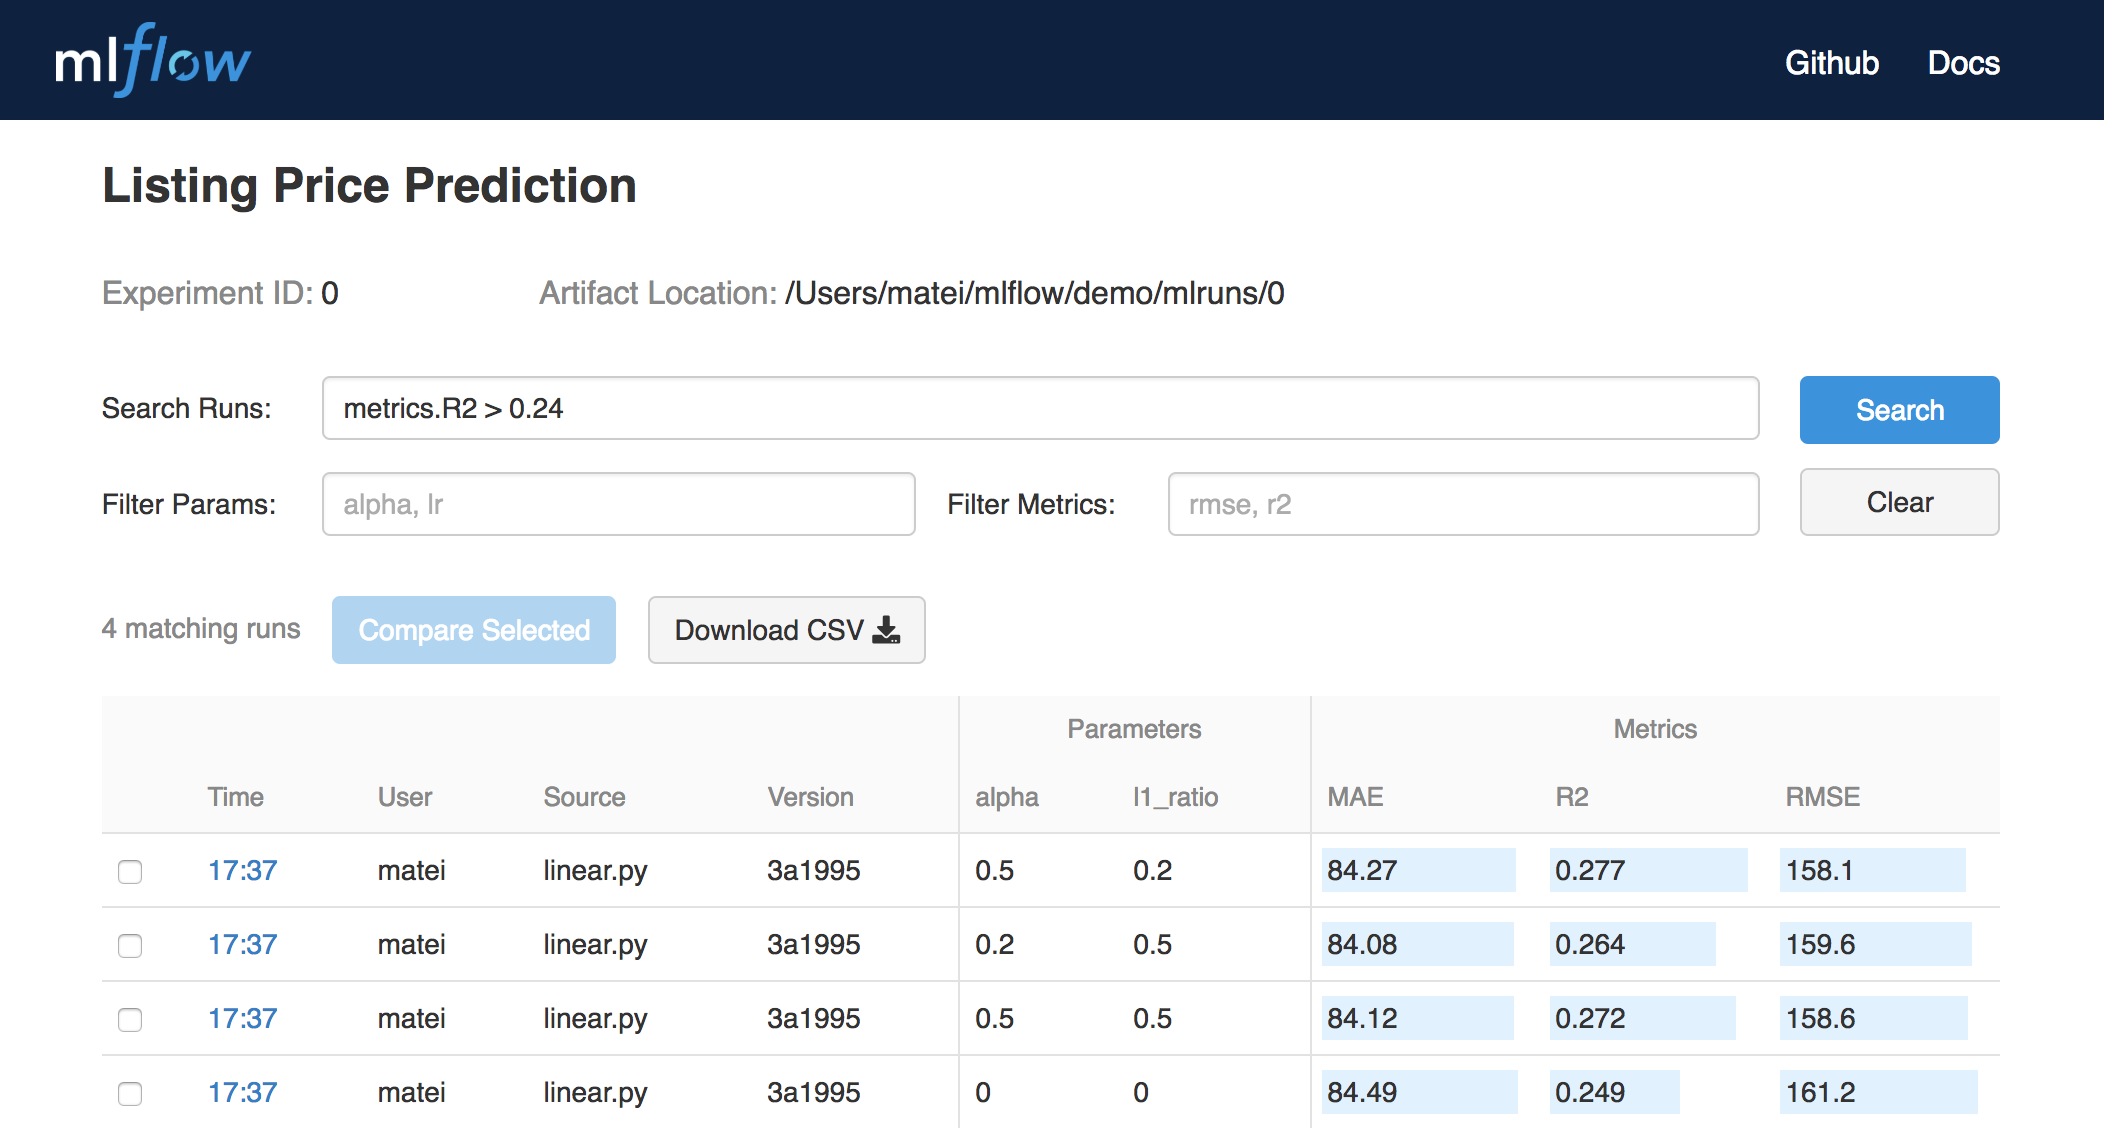
\includegraphics[bb=0 0 1052 564,width=\textwidth]{tracking.png}
\caption{MLflow Tracking UI showing several runs in an experiment. Clicking each run lists its metrics, artifacts and output details and lets the user post comments about the run.}
\label{fig:tracking-ui}
\end{figure}

\subsection{MLflow Projects}

MLflow Projects provide a simple format for packaging reproducible data science code. Each project is simply a directory with code or a Git repository, and uses a descriptor file to specify its dependencies and how to run the code. A MLflow Project is defined by a simple YAML file called MLproject, as shown below:

\begin{Verbatim}[frame=single,fontsize=\small,samepage=true]
name: My Project
conda_env: conda.yaml
entry_points:
  main:
    parameters:
      data_file: path
      alpha: {type: float, default: 0.1}
    command: "python train.py --reg-param {alpha} --data {data_file}"
\end{Verbatim}


Projects can specify their dependencies through a Conda environment or (in an upcoming release) a Docker container specification. A project may also have multiple entry points for invoking runs, with named parameters that downstream users can provide without understanding the internals of the project.

Users can run projects using the \texttt{mlflow run} command line tool, either from local files or a Git repository:

\begin{Verbatim}[frame=single,fontsize=\small,samepage=true]
mlflow run git@github.com:databricks/mlflow-example.git -P alpha=0.5
\end{Verbatim}

Alternatively, projects can be called programmatically using MLflow's API. This can be used to implement multi-step workflows or to pass projects a ``black box'' into automated tools such as hyperparameter search~\cite{hyperopt}.

In either case, MLflow will automatically set up the project's runtime environment and execute it. If the code inside the project uses the MLflow Tracking API, MLflow will also remember the project version executed (that is, the Git commit) and show an \texttt{mlflow run} command to re-execute it in its UI. Finally, MLflow projects can also be submitted to cloud platforms such as Databricks for remote execution.

\subsection{MLflow Models}

MLflow Models are a convention for packaging machine learning models in multiple formats called ``flavors'', allowing diverse tools to understand the model at different levels of abstractions. MLflow also offers a variety of built-in tools to deploy models in its standard favors. For example, the same model can be deployed as a Docker container for REST serving, as an Apache Spark user-defined function (UDF) for batch inference, or into cloud-managed serving platforms like Amazon SageMaker and Azure ML.

Each MLflow Model is simply stored as a directory containing arbitrary files and an MLmodel YAML file that lists the flavors it can be used in and additional metadata about how it was created:

\begin{Verbatim}[frame=single,fontsize=\small,samepage=true]
time_created: 2018-02-21T13:21:34.12
run_id: c4b65fc2c57f4b6d80c6e58a9dcb9f01
flavors:
  sklearn:
    sklearn_version: 0.19.1
    pickled_model: model.pkl
  python_function:
    loader_module: mlflow.sklearn
    pickled_model: model.pkl
\end{Verbatim}

In this example, the model can be used with tools that support either the \texttt{sklearn} or \texttt{python\_function} model flavors. For example, the MLflow SciKit-Learn library knows how to load a \texttt{sklearn} model as a SciKit-Learn Python object, but other deployment tools, such as running the model in a Docker HTTP server, only understand lower-level flavors like \texttt{python\_function}.
In addition, models logged using MLflow Tracking APIs will automatically include a reference to that run's unique ID, letting users discover how they were built.

\section{Example Use Cases}

In this section, we describe three sample MLflow use cases to highlight how users can leverage each component.

\vspace{-0.6em}
\paragraph{Experiment tracking.} A European energy company is using MLflow to track and update hundreds of energy grid models. This team's goal is to build a time series model for every major energy producer (e.g., power plant) and consumer (e.g., factory), monitor these using standard metrics, and combine the predictions to drive business processes such as pricing. Because a single team is responsible for hundreds of models, possibly using different ML libraries, it was important to have a standard development and tracking process. The team has standardized on using Jupyter notebooks for development, MLflow Tracking for metrics, and Databricks jobs for inference.

\vspace{-0.6em}
\paragraph{Reproducible projects.} An online marketplace is using MLflow Projects to package deep learning jobs using Keras and run them in the cloud. Each data scientist develops models locally on his or her laptop using a small dataset, checks them into a Git repository with an MLproject file, and submits remote runs of the project to GPU instances in the cloud for large-scale training or hyperparameter search. Using MLflow Projects makes it easy to create the same software environment in the cloud and share project code between different data scientists.

\vspace{-0.6em}
\paragraph{Model packaging.} The data science team at an e-commerce site is using MLflow Models to package recommendation models for use by application engineers. The technical challenge here was that the recommendation application includes both a standard, ``off-the-shelf'' recommendation model and custom business logic for pre- and post-processing. For example, the application might include custom code to make sure that the recommended items are diverse. This business logic needs to change in sync with the model, and the data science team wants to control both the business logic and the model, without having to submit a patch to the web application each time this logic has to change.
Moreover, the team wants to A/B test distinct models with distinct versions of the processing logic.
The solution was to package both the recommendation model and the custom logic using the \texttt{python\_function} flavor in an MLflow Model, which can then be deployed and tested as a single unit. %This allows production engineers to deploy the recommendation code as they please without the processing logic falling out of sync with the model.

\section{Related Work}

Many software systems aim to simplify ML development.
The closest to our work are the end-to-end ``ML platforms'' at large web companies.
For example, Facebook's FBLearner lets users write reusable workflow steps that run over data in Apache Hive~\cite{fblearner};
Uber's Michelangelo gives users a toolkit of algorithms to choose from that it can automatically train and deploy~\cite{michelangelo}; and Google's TFX provides data preparation and serving tools around TensorFlow~\cite{tfx}.
Anecdotally, these platforms greatly accelerate ML development, showing the benefits of standardizing the ML lifecycle.
However, they generally restrict users to a specific set of algorithms or libraries, so teams are on their own when they step outside these boundaries.
Our goal in MLflow is to let users easily bring their own tools and software in as many steps in the process as possible through our ``open interface'' design.
This includes custom training steps, inference code, and logged parameters and artifacts.

Other systems also tackle specific problems within the ML lifecycle. For example, Sacred~\cite{sacred}, ModelDB~\cite{modeldb} and TensorBoard~\cite{tensorboard} let users track experiments; PMML~\cite{pmml} and ONNX~\cite{onnx} are cross-library model serialization formats; Clipper~\cite{clipper} can deploy arbitrary models as Docker containers; and CDE~\cite{cde}, CodaLab~\cite{codalab}, Binder~\cite{binder} and Repo2Docker~\cite{repo2docker} enable reproducible software runs. MLflow combines these concepts with new ones, such as multi-flavor model packaging, into a unified system design and API.

\section{Conclusion}

For machine learning to have widespread commercial impact, organizations require the same kinds of reliable engineering processes around ML that exist in other engineering disciplines such as software development. In this paper, we have described some of the key challenges that differentiate ML development from traditional software development, such as experimentation, reproducibility, and reliable production deployment. We have also described MLflow, a software platform that can structure the machine learning lifecycle while giving users broad flexibility to use their own ML algorithms, software libraries and development processes.
MLflow is available as open source software at \url{https://www.mlflow.org}.


{\small

\begin{thebibliography}{10}

  \bibitem{abadi2016tensorflow}
  M.~Abadi, P.~Barham, J.~Chen, Z.~Chen, A.~Davis, J.~Dean, M.~Devin,
    S.~Ghemawat, G.~Irving, M.~Isard, et~al.
  \newblock {TensorFlow: A System for Large-Scale Machine Learning}.
  \newblock In {\em OSDI}, volume~16, pages 265--283, 2016.

  \bibitem{tfx}
  D.~Baylor, E.~Breck, H.-T. Cheng, N.~Fiedel, C.~Y. Foo, Z.~Haque, S.~Haykal,
    M.~Ispir, V.~Jain, L.~Koc, C.~Y. Koo, L.~Lew, C.~Mewald, A.~N. Modi,
    N.~Polyzotis, S.~Ramesh, S.~Roy, S.~E. Whang, M.~Wicke, J.~Wilkiewicz,
    X.~Zhang, and M.~Zinkevich.
  \newblock Tfx: A tensorflow-based production-scale machine learning platform.
  \newblock In {\em Proceedings of the 23rd ACM SIGKDD International Conference
    on Knowledge Discovery and Data Mining}, KDD '17, pages 1387--1395, New York,
    NY, USA, 2017. ACM.

  \bibitem{hyperopt}
  J.~Bergstra, B.~Komer, C.~Eliasmith, D.~Yamins, and D.~D. Cox.
  \newblock Hyperopt: a python library for model selection and hyperparameter
    optimization.
  \newblock {\em Computational Science and Discovery}, 8(1):014008, 2015.

  \bibitem{binder}
  {Binder}.
  \newblock \url{https://mybinder.org}, 2018.

  \bibitem{clipper}
  D.~Crankshaw, X.~Wang, G.~Zhou, M.~J. Franklin, J.~E. Gonzalez, and I.~Stoica.
  \newblock Clipper: A low-latency online prediction serving system.
  \newblock In {\em Proceedings of the 14th USENIX Conference on Networked
    Systems Design and Implementation}, NSDI'17, pages 613--627, Berkeley, CA,
    USA, 2017. USENIX Association.

  \bibitem{fblearner}
  J.~Dunn.
  \newblock Introducing {FBLearner Flow}: Facebook’s {AI} backbone.
  \newblock
    \url{https://code.fb.com/core-data/introducing-fblearner-flow-facebook-s-ai-backbone/}.

  \bibitem{repo2docker}
  J.~Forde, T.~Head, C.~Holdgraf, Y.~Panda, G.~Nalvarte, M.~Pacer, F.~Perez,
    B.~Ragan-Kelley, and E.~Sundell.
  \newblock Reproducible research environments with repo2docker.
  \newblock ICML, 07/2018 2018.

  \bibitem{tensorboard}
  Google.
  \newblock Tensorboard: Visualizing learning.
  \newblock \url{https://www.tensorflow.org/guide/summaries_and_tensorboard}.

  \bibitem{pmml}
  A.~Guazzelli, W.-C. Lin, and T.~Jena.
  \newblock {\em PMML in Action: Unleashing the Power of Open Standards for Data
    Mining and Predictive Analytics}.
  \newblock CreateSpace, Paramount, CA, 2nd edition, 2012.

  \bibitem{cde}
  P.~J. Guo.
  \newblock {CDE}: A tool for creating portable experimental software packages.
  \newblock {\em Computing in Science and Engineering}, 14(4):32--35, 2012.

  \bibitem{michelangelo}
  J.~Hermann and M.~D. Balso.
  \newblock Meet {Michelangelo}: Uber’s machine learning platform.
  \newblock \url{https://eng.uber.com/michelangelo/}.

  \bibitem{sacred}
  {K}laus {G}reff, {A}aron {K}lein, {M}artin {C}hovanec, {F}rank {H}utter, and
    {J}\"urgen {S}chmidhuber.
  \newblock {T}he {S}acred {I}nfrastructure for {C}omputational {R}esearch.
  \newblock In {K}aty {H}uff, {D}avid {L}ippa, {D}illon {N}iederhut, and
    M.~{P}acer, editors, {\em {P}roceedings of the 16th {P}ython in {S}cience
    {C}onference}, pages 49 -- 56, 2017.

  \bibitem{codalab}
  P.~Liang et~al.
  \newblock {CodaLab}.
  \newblock \url{https://worksheets.codalab.org}, 2018.

  \bibitem{onnx}
  {ONNX Group}.
  \newblock {ONNX}.
  \newblock \url{https://onnx.ai}.

  \bibitem{modeldb}
  M.~Vartak, H.~Subramanyam, W.-E. Lee, S.~Viswanathan, S.~Husnoo, S.~Madden, and
    M.~Zaharia.
  \newblock Modeldb: A system for machine learning model management.
  \newblock In {\em Proceedings of the Workshop on Human-In-the-Loop Data
    Analytics}, HILDA '16, pages 14:1--14:3, New York, NY, USA, 2016. ACM.

  \end{thebibliography}


}
%\bibliographystyle{abbrv}
%\bibliography{paper}

\end{document}

\end{article}



\begin{article}
{From the Edge to the Cloud: Model Serving in ML.NET}
{Yunseong Lee, Alberto Scolari, Byung-Gon Chun, Markus Weimer, Matteo Interlandi}
\graphicspath{{submissions/model_serving_dot_net/figs/}}
\pdfminorversion=5
\documentclass[11pt]{article}
\usepackage{deauthor,times,graphicx,caption,microtype}
\usepackage{hyperref}
\usepackage{listings}
\usepackage{booktabs}

\begin{document}

\title{Optimistic Lock Coupling: A Scalable and Efficient General-Purpose Synchronization Method}

\author{Viktor Leis, Michael Haubenschild\raisebox{0.9ex}{$\ast$}, Thomas Neumann\\ Technische Universit{\"a}t M{\"u}nchen \hspace{0.7cm} Tableau Software\raisebox{0.9ex}{$\ast$} \\ {\{leis,neumann\}{@}in.tum.de} \hspace{0.7cm} {mhaubenschild{@}tableau.com\raisebox{0.9ex}{$\ast$}}}

\maketitle

\begin{abstract}
As the number of cores on commodity processors continues to increase, scalability becomes more and more crucial for overall performance.
Scalable and efficient concurrent data structures are particularly important, as these are often the building blocks of parallel algorithms.
Unfortunately, traditional synchronization techniques based on fine-grained locking have been shown to be unscalable on modern multi-core CPUs.
Lock-free data structures, on the other hand, are extremely difficult to design and often incur significant overhead.

In this work, we make the case for Optimistic Lock Coupling as a practical alternative to both traditional locking and the lock-free approach.
We show that Optimistic Lock Coupling is highly scalable and almost as simple to implement as traditional lock coupling.
Another important advantage is that it is easily applicable to most tree-like data structures.
We therefore argue that Optimistic Lock Coupling, rather than a complex and error-prone custom synchronization protocol, should be the default choice for performance-critical data structures.
\end{abstract}

\section{Introduction}

% more and more cores
Today, Intel's commodity server processors have up to 28 cores and its upcoming microarchitecture will have up to 48 cores per socket~\cite{intel}.
Similarly, AMD currently stands at 32 cores and this number is expected to double in the next generation~\cite{amd}.
Since both platforms support simultaneous multithreading (also known as hyperthreading), affordable commodity servers (with up to two sockets) will soon routinely have between 100 and 200 hardware threads.

% data structure scalability is important
With such a high degree of hardware parallelism, efficient data processing crucially depends on how well concurrent data structures scale.
Internally, database systems use a plethora of data structures like table heaps, internal work queues, and, most importantly, index structures.
Any of these can easily become a scalability (and therefore overall performance) bottleneck on many-core CPUs.

% traditional synchronization: fine-grained locks, slow, cache invalidation
Traditionally, database systems synchronize internal data structures using fine-grained reader/writer locks\footnote{In this work, we focus on data structure synchronization rather than high-level transaction semantics and therefore use the term {\em lock} for what would typically be called {\em latch} in the database literature. We thus follow common computer science (rather than database) terminology.}.
Unfortunately, while fine-grained locking makes lock contention unlikely, it still results in bad scalability because lock acquisition and release require writing to shared memory.
Due to the way cache coherency is implemented on modern multi-core CPUs, these writes cause additional cache misses\footnote{The cache coherency protocol ensures that all copies of a cache line on other cores are invalidated before the write can proceed.} and the cache line containing the lock's internal data becomes a point of physical contention.
As a result, any frequently-accessed lock (e.g., the lock of the root node of a B-tree) severely limits scalability.

% lock-free bw-tree: no more latches, but indirections, extremely complex
Lock-free data structures like the Bw-tree~\cite{DBLP:conf/icde/LevandoskiLS13a} (a lock-free B-tree variant) or the Split-Ordered List~\cite{DBLP:journals/jacm/ShalevS06} (a lock-free hash table) do not acquire any locks and therefore generally scale much better than locking-based approaches (in particular for read-mostly workloads).
However, lock-free synchronization has other downsides:
First, it is very difficult and results in extremely complex and error-prone code (when compared to locking).
Second, because the functionality of atomic primitives provided by the hardware (e.g., atomically compare-and-swap 8 bytes) is limited, complex operations require additional indirections within the data structure.
For example, the Bw-tree requires an indirection table and the Split-Ordered List requires ``dummy nodes'', resulting in overhead due to additional cache misses.

% OLC for the win
In this paper we make the case for {\em Optimistic Lock Coupling (OLC)}, a synchronization method that combines some of the best properties of lock-based and lock-free synchronization.
OLC utilizes a special lock type that can be used in two modes:
The first mode is similar to a traditional mutex and excludes other threads by physically acquiring the underlying lock.
In the second mode, reads can proceed optimistically by validating a version counter that is embedded in the lock (similar to optimistic concurrency control).
The first mode is typically used by writers and the second mode by readers.
Besides this special lock type, OLC is based on the observation that optimistic lock validations can be interleaved/coupled---similar to the pair-wise interleaved lock acquisition of traditional lock coupling.
Hence, the name Optimistic Lock Coupling.

OLC has a number of desirable features:
\begin{itemize}
\item By reducing the number of writes to shared memory locations and thereby avoiding cache invalidations, it {\bf scales well} for most workloads.
\item In comparison to unsynchronized code, it requires few additional CPU instructions making it {\bf efficient}.
\item OLC is {\bf widely applicable} to different data structures. It has already been successfully used for synchronizing binary search trees~\cite{DBLP:conf/ppopp/BronsonCCO10}, tries~\cite{artsync}, trie/B-tree hybrids~\cite{DBLP:dblp_conf/eurosys/MaoKM12}, and B-trees~\cite{buzzword}.
\item In comparison to the lock-free paradigm, it is also {\bf easy to use} and requires few modifications to existing, single-threaded data structures.
\end{itemize}
Despite these positive features and its simplicity, OLC is not yet widely known.
The goal of this paper is therefore to popularize this simple idea and to make a case for it.
We argue that OLC deserves to be widely known.
It is a good default synchronization paradigm---more complex, data structure-specific protocols are seldom beneficial.

The rest of the paper is organized as follows.
Section~\ref{sec:related} discusses related work, tracing the history of OLC and its underlying ideas in the literature.
The core of the paper is Section~\ref{sec:olc}, which describes the ideas behind OLC and how it can be used to synchronize complex data structures.
In Section~\ref{sec:evaluation} we experimentally show that OLC has low overhead and scales well when used to synchronize an in-memory B-tree.
We summarize the paper in Section~\ref{sec:conc}.

\newpage
\section{Related Work}\label{sec:related}

Lock coupling has been proposed as a method for allowing concurrent operations on B-trees in 1977~\cite{DBLP:journals/acta/BayerS77}.
This traditional and still widely-used method, described in detail in Graefe's B-tree survey~\cite{DBLP:journals/ftdb/Graefe11}, is also called ``latch coupling'', ``hand-over-hand locking'', and ``crabbing''.
Because at most two locks are held at-a-time during tree traversal, this technique seemingly allows for a high degree of parallelism---in particular if read/write locks are used to enable inner nodes to be locked in shared mode.
However, as we show in Section~\ref{sec:evaluation}, on modern hardware lock acquisition (even in shared mode) results in suboptimal scalability.

An early alternative from 1981 is a B-tree variant called B-link tree~\cite{DBLP:journals/tods/LehmanY81}, which only holds a single lock at a time.
It is based on the observation that between the release of the parent lock and the acquisition of the child lock, the only ``dangerous'' thing that could have happened is the split of a child node (assuming one does not implement merge operations).
Thus, when a split happens, the key being searched might end up on a neighboring node to the right of the current child node.
A B-link tree traversal therefore detects this condition and, if needed, transparently proceeds to the neighboring node.
Releasing the parent lock early is highly beneficial when the child node needs to be fetched from disk.
For in-memory workloads, however, the B-link tree has the same scalability issues as lock coupling (it acquires just as many locks).

The next major advance, Optimistic Latch-Free Index Traversal (OLFIT)~\cite{DBLP:conf/vldb/ChaHKK01}, was proposed in 2001.
OLFIT introduced the idea of a combined lock/update counter, which we call {\em optimistic lock}. % , for lack of a better name,
Based on these per-node optimistic locks and the synchronization protocol of the B-link tree, OLFIT finally achieves good scalability on parallel processors.
The OLFIT protocol is fairly complex, as it requires both the non-trivial B-link protocol and optimistic locks.
Furthermore, like the B-link tree protocol, it does not support merging nodes, and is specific to B-trees (cannot easily be applied to other data structures).

In the following two decades, the growth of main-memory capacity led to much research into other data structures besides the venerable B-tree.
Particularly relevant for our discussion is Bronson et al.'s~\cite{DBLP:conf/ppopp/BronsonCCO10} concurrent binary search tree, which is based on optimistic version validation and has a sophisticated, data structure-specific synchronization protocol.
To the best of our knowledge, this 2010 paper is the first that, as part of its protocol, interleaves version validation across nodes---rather than validating each node separately like OLFIT.
In that paper, this idea is called ``hand-over-hand, optimistic validation'', while we prefer the term Optimistic Lock Coupling to highlight the close resemblance to traditional lock coupling.
Similarly, Mao et al.'s~\cite{DBLP:dblp_conf/eurosys/MaoKM12} Masstree (a concurrent hybrid trie/B-tree) is also based on the same ideas, but again uses them as part of a more complex protocol.

The Adaptive Radix Tree (ART)~\cite{art} is another recent in-memory data structure, which we proposed in 2013.
In contrast to the two data structures just mentioned, it was originally designed with single-threaded performance in mind without supporting concurrency.
To add support for concurrency, we initially started designing a custom protocol called Read-Optimized Write Exclusion (ROWEX)~\cite{artsync}, which turned out to be non-trivial and requires modifications of the underlying data structure\footnote{Note that ROWEX is already easier to apply to existing data structures than the lock-free approach. The difficulty depends on the data structure. Applying ROWEX is hard for B-trees with sorted keys and fairly easy for copy-on-write data structures like the Height Optimized Trie~\cite{hot}---with ART being somewhere in the middle.}.
However, fairly late in the project, we also realized, that OLC {\em alone} (rather than as part of a more complex protocol) is sufficient to synchronize ART.
No other changes to the data structure were necessary.
Both approaches were published and experimentally evaluated in a followup paper~\cite{artsync}, which shows that, despite its simplicity, OLC is efficient, scalable, and generally outperforms ROWEX.

Similar results were recently published regarding B-trees~\cite{buzzword}.
In this experimental study a simple OLC-based synchronization outperformed the Bw-tree~\cite{DBLP:conf/icde/LevandoskiLS13a}, a complex lock-free synchronization approach.
Another recent paper shows that for write-intensive workloads, locking often performs better than lock-free synchronization~\cite{DBLP:conf/cidr/FaleiroA17}.
These experiences indicate that OLC is a general-purpose synchronization paradigm and motivate the current paper.

%foster b-tree\cite{DBLP:journals/tods/GraefeKK12}
%Shasha theory~\cite{DBLP:journals/tods/ShashaG88}

\section{Optimistic Lock Coupling}\label{sec:olc}

% locks suck
The standard technique for inter-thread synchronization is mutual exclusion using fine-grained locks.
In a B-tree, for example, every node usually has its own associated lock, which is acquired before accessing that node.
The problem of locking on modern multi- and many-core processors is that lock acquisition and release require writing to the shared memory location that implements the lock.
This write causes exclusive ownership of the underlying cache line and invalidates copies of it on all other processor cores.
For hierarchical, tree-like data structures, the lock of the root node becomes a point of physical contention---even in read-only workloads and even when read/write locks are used.
Depending on the specific data structure, number of cores, cache coherency protocol implementation, cache topology, whether Non-Uniform Memory Access (NUMA) is used, locking can even result in multi-threaded performance that is worse than single-threaded execution.

% in b-trees this happens very much
The inherent pessimism of locking is particularly unfortunate for B-trees:
Despite the fact that logical modifications of the root node are very infrequent, every B-tree operation must lock the root node during tree traversal\footnote{To a lesser extent this obviously applies to all inner nodes, not just the root.}.
Even the vast majority of update operations (with the exception of splits and merges), only modify a single leaf node.
These observations indicate that a more optimistic approach, which does not require locking inner nodes, would be very beneficial for B-trees.

\subsection{Optimistic Locks}

% optimism to the rescue
As the name indicates, optimistic locks try to solve the scalability issues of traditional locks using an optimistic approach.
Instead of always physically acquiring locks, even for nodes that are unlikely to be modified simultaneously, after-the-fact validation is used to detect conflicts.
This is done by augmenting each lock with a version/update counter that is incremented on every modification.
Using this version counter, readers can optimistically proceed before validating that the version did not change to ensure that the read was safe.
If validation fails, the operation is restarted.

% details on opt locks
Using optimistic locks, a read-only node access (i.e., the majority of all operations in a B-tree) does not acquire the lock and does not increment the version counter.
Instead, it performs the following steps:
\begin{enumerate}
\item read lock version (restart if lock is not free)
\item access node
\item read the version again and validate that it has not changed in the meantime
\end{enumerate}
If the last step (the validation) fails, the operation has to be restarted.
Write operations, on the other hand, are more similar to traditional locking:
\begin{enumerate}
\item acquire lock (wait if necessary)
\item access/write to node
\item increment version and unlock node
\end{enumerate}
Writes can therefore protect a node from other writes.

% similar to locks
As we observed in an earlier paper~\cite{artsync}, because of similar semantics, optimistic locks can be hidden behind an API very similar to traditional read/write locks.
Both approaches have an exclusive lock mode, and acquiring a traditional lock in shared mode is analogous to optimistic version validation.
Furthermore, like with some implementations of traditional read/write locks, optimistic locks allow upgrading a shared lock to an exclusive lock.
Lock upgrades are, for example, used to avoid most B-tree update operations from having to lock inner nodes.
In our experience, the close resemblance of optimistic and traditional locks simplifies the reasoning about optimistic locks;
one can apply similar thinking as in traditional lock-based protocols.

\subsection{Lock Coupling with Optimistic Locks}

\begin{figure}
  \centering
  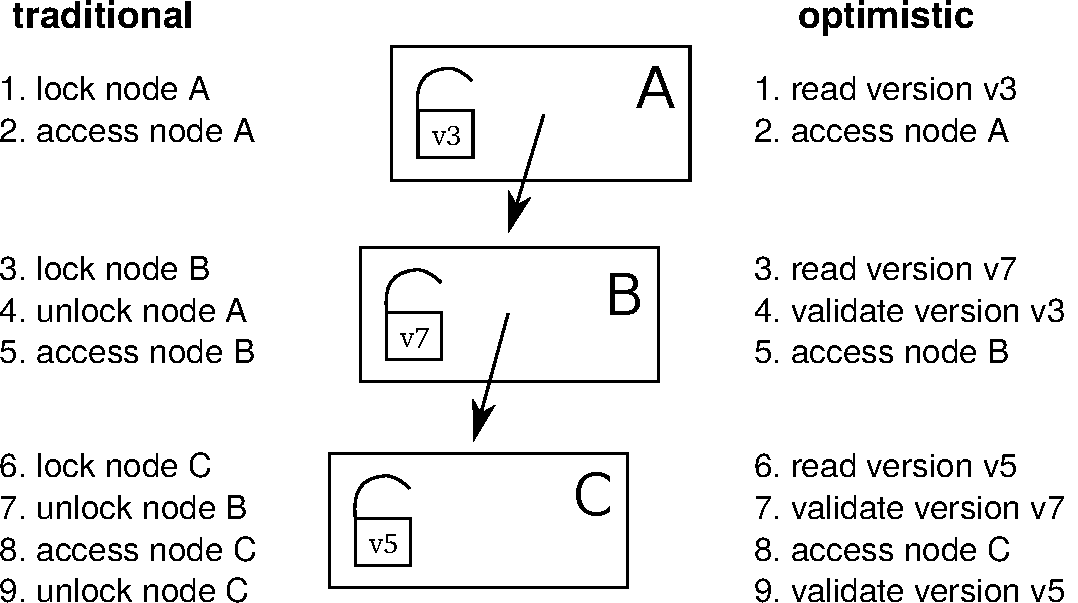
\includegraphics[width=0.65\linewidth]{olcall.pdf}
  \vspace{0.2cm}
  \caption{Comparison of a lookup operation in a 3-level tree using traditional lock coupling (left-hand side) vs.~optimistic lock coupling (right-hand side).}
  \label{fig:olc}
\end{figure}

The traditional and most common lock-based synchronization protocol for B-trees is lock coupling, which interleaves lock acquisitions while holding at most two locks at a time.
If, as we observed earlier, optimistic locks have similar semantics as traditional locks, it is natural to ask whether lock coupling can be combined with optimistic locks.
And indeed the answer is yes: One can almost mechanically translate traditional lock coupling code to optimistic lock coupling code.
This is illustrated in Figure~\ref{fig:olc}, which compares the traversal in a tree of height 3 using traditional and optimistic locks.
As the figure shows, the main difference is that locking is translated to reading the version and that unlocking becomes validation of the previously read version.
This simple change provides efficient lock-free tree traversal without the need to design a complex synchronization protocol.

It is important to emphasize the conceptual simplicity of OLC in comparison to data structures that use custom protocols like the Bw-tree~\cite{DBLP:conf/icde/LevandoskiLS13a}.
To implement lock-free access, the Bw-tree requires an indirection table, delta nodes, complex splitting and merging logic, retry logic, etc.
OLC, on the other hand, can directly be applied to B-trees mostly by adding the appropriate optimistic locking code and without modifying the node layout itself.
Therefore, OpenBw-Tree, an open source implementation of the Bw-tree, requires an order of magnitude more code than a B-tree based on OLC\footnote{Both implementations are available on GitHub: \url{https://github.com/wangziqi2016/index-microbench}}.
Given how difficult it is to develop, validate, and debug lock-free code, simplicity is obviously a major advantage.

\subsection{Correctness Aspects}

\begin{figure}
  % \centering
  %[basicstyle=\normalsize\ttfamily,showstringspaces=false,columns=fullflexible,breaklines=false,breakatwhitespace=true,numbers=none,numberstyle=\small,style=C,keepspaces=true]
\begin{lstlisting}[basicstyle=\ttfamily,language=C++,numbers=left,numberstyle=\small]
std::atomic<BTreeNode*> root;

// search for key in B+tree, returns payload in resultOut
bool lookup(Key key, Value& resultOut) {
   BTreeNode* node = root.load();
   uint64_t nodeVersion = node->readLockOrRestart();
   if (node != root.load()) // make sure the root is still the root
      restart();

   BTreeInner<Key>* parent = nullptr;
   uint64_t parentVersion = 0;

   while (node->isInner()) {
      auto inner = (BTreeInner*)node;

      // unlock parent and make current node the parent
      if (parent)
         parent->readUnlockOrRestart(parentVersion);
      parent = inner;
      parentVersion = nodeVersion;

      // search for next node
      node = inner->findChild(key);
      // validate 'inner' to ensure that 'node' pointer is valid
      inner->checkOrRestart(nodeVersion);
      // now it safe to dereference 'node' pointer (read its version)
      nodeVersion = node->readLockOrRestart();
   }

   // search in leaf and retrieve payload
   auto leaf = (BTreeLeaf*)node;
   bool success = leaf->findValue(key, resultOut);

   // unlock everything
   if (parent)
      parent->readUnlockOrRestart(parentVersion);
   node->readUnlockOrRestart(nodeVersion);

   return success;
}
\end{lstlisting}
  \vspace{0.2cm}
  \caption{B-tree lookup code using OLC. For simplicity, the restart logic is not shown.}
  \label{fig:lookup}
\end{figure}

So far, we have introduced the high-level ideas behind OLC and have stressed its similarity to traditional lock coupling.
Let us now discuss some cases where the close similarity between lock coupling and OLC breaks down.
To make this more concrete, we show the B-tree lookup code in Figure~\ref{fig:lookup}.
In the code, \texttt{readLockOrRestart} reads the lock version and \texttt{readUnlockOrRestart} validates that the read was correct.

One issue with OLC is that any pointer speculatively read from a node may point to invalid memory (if that node is modified concurrently).
Dereferencing such a pointer (e.g., to read its optimistic lock), may cause a segmentation fault or undefined behavior.
In the code shown in Figure~\ref{fig:lookup}, this problem is prevented by the extra check in line 25, which ensures that the read from the node containing the pointer was correct.
Without this additional validation, the code would in line 27 dereference the pointer speculatively read in line 23.
Note that the implementation of \texttt{checkOrRestart} is actually identical to \texttt{readUnlockOrRestart}.
We chose to give it a different name to highlight the fact that this extra check would not be necessary with read/write locks.

Another potential issue with optimistic locks is code that does not terminate.
Code that speculatively accesses a node, like an intra-node binary search, should be written in a way such that it always terminates---even in the presence of concurrent writes.
Otherwise, the validation code that detects the concurrent write will never run.
The binary search of a B-tree, for example, needs to be written in such a way that each comparison makes progress.
For some data structures that do not require loops in the traversal code (like ART) termination is trivially true.

\subsection{Implementation Details}

% implementation, efficiency
To implement an optimistic lock, one can combine the lock and the version counter into a single 64-bit\footnote{Even after subtracting one bit for the lock status, a back-of-the-envelope calculation can show that 63 bits are large enough to never overflow in practice.} word~\cite{artsync}.
A typical read operation will therefore merely consist of reading this version counter atomically.
In C++11 this can be implemented using the \texttt{std::atomic} type.

On x86, atomic reads are cheap because of x86's strong memory order guarantees.
No memory fences are required for sequentially-consistent loads, which are translated (by both GCC and clang) into standard \texttt{MOV} instructions.
Hence, the only effect of \texttt{std::atomic} for loads is preventing instruction re-ordering.
This makes version access and validation cheap.
Acquiring and releasing an optimistic lock in exclusive mode has comparable cost to a traditional lock:
A fairly expensive sequentially-consistent store is needed for acquiring a lock, while a standard \texttt{MOV} suffices for releasing it.
A simple sinlock-based implementation of optimistic locks can be found in the appendix of an earlier paper~\cite{artsync}.

OLC code must be able to handle restarts since validation or lock upgrade can fail due to concurrent writers.
Restarts can easily be implemented by wrapping the data structure operation in a loop (for simplicity not shown in Figure~\ref{fig:lookup}).
Such a loop also enables limiting the number of optimistic retry operations and falling back to pessimistic locking in cases of very heavy contention.
The ability to fall back to traditional locking is a major advantage of OLC in terms of robustness over lock-free approaches, which do not have this option.

In addition to the optimistic shared mode and the exclusive mode, optimistic locks also support a ``shared pessimistic'' mode, which physically acquires the lock in shared mode (allowing multiple concurrent readers but no writers).
This mode is useful for table (or range) scans that touch many tuples on a leaf page (which would otherwise easily abort).
Finally, let us mention that large range scans and table scans, should be broken up into several per-node traversals as is done in the LeanStore~\cite{leanstore} system.

Like all lock-free data structures, but unlike traditional locking and Hardware Transactional Memory~\cite{DBLP:conf/hpca/KarnagelDRLLSL14,DBLP:journals/pvldb/MakreshanskiLS15,htmtkde}, OLC requires care when deleting (and reusing) nodes.
The reason is that a deleting thread can never be sure that a node can be reclaimed because other threads might still be optimistically reading from that node.
Therefore, standard solutions like epoch-based reclamation~\cite{DBLP:conf/sosp/TuZKLM13}, hazard pointers~\cite{DBLP:journals/tpds/Michael04}, or optimized hazard pointers~\cite{DBLP:conf/spaa/BalmauGHZ16} need to be used.
These memory reclamation techniques are, however, largely orthogonal to the synchronization protocol itself.

%-lock-free is not a strong guarantee

\newpage
\section{Evaluation}\label{sec:evaluation}

Let us now experimentally evaluate the overhead and scalability of OLC.
For the experiments, we use an in-memory B+tree implemented in C++11 using templates, which is configured to use nodes of 4096 bytes, random 8 byte keys, and 8 byte payloads.
Based on this B-tree, we compare the following synchronization approaches:
\begin{itemize}
\item an OLC implementation\footnote{An almost identical OLC implementation is available on github: \url{https://github.com/wangziqi2016/index-microbench/tree/master/BTreeOLC}}
\item a variant based on traditional lock coupling and read/write locks
\item the unsynchronized B-tree, which obviously is only correct for read-only workloads but allows measuring the overhead of synchronization
\end{itemize}
Note that earlier work has compared the OLC implementation with a Bw-tree implementation~\cite{buzzword} and other state-of-the-art in-memory index structures.

We use a Haswell EP system with an Intel Xeon E5-2687W v3 CPU, which has 10 cores (20 ``Hyper-Threads'') and 25~MB of L3 cache.
The system is running Ubuntu 18.10 and we use GCC 8.2.0 to compile our code.
The CPU counters are obtained using the Linux perf API\footnote{We use the following convenience wrapper: \url{https://github.com/viktorleis/perfevent}}.

\begin{table}
  \caption{Performance and CPU counters for lookup and insert operations in a B-tree with 100M keys. We perform 100M operations and normalize the CPU counters by that number.}
  \label{tab:overhead}
  \centering
  \begin{tabular}{lrrrrrrr}\toprule
                    &         &        &        & instruc-  & L1     & L3     & branch \\
                    & threads & M op/s & cycles & tions & misses & misses & misses \\\midrule
lookup (no sync.)   & 1       & 1.72   & 2028   & 283     & 39.1   & 14.9   & 16.1   \\
lookup (OLC)        & 1       & 1.65   & 2107   & 370     & 43.9   & 15.1   & 16.7   \\
lookup (lock coup.) & 1       & 1.72   & 2078   & 365     & 42.3   & 16.9   & 15.7   \\\midrule
insert (no sync.)   & 1       & 1.51   & 2286   & 530     & 59.8   & 31.1   & 17.3   \\
insert (OLC)        & 1       & 1.50   & 2303   & 629     & 61.2   & 31.1   & 16.5   \\
insert (lock coup.) & 1       & 1.41   & 2473   & 644     & 61.0   & 31.0   & 17.2   \\\midrule
lookup (no sync.)   & 10      & 15.48  & 2058   & 283     & 38.6   & 15.5   & 16.0   \\
lookup (OLC)        & 10      & 14.60  & 2187   & 370     & 43.8   & 15.8   & 16.8   \\
lookup (lock coup.) & 10      & 5.71   & 5591   & 379     & 54.2   & 17.0   & 14.8   \\\midrule
insert (no sync.)   & 10      & -      & -      & -       & -      & -      & -      \\
insert (OLC)        & 10      & 10.46  & 2940   & 656     & 62.0   & 32.5   & 16.8   \\
insert (lock coup.) & 10      & 7.55   & 4161   & 667     & 75.0   & 28.6   & 16.2   \\
    \bottomrule
\end{tabular}
\end{table}

Table~\ref{tab:overhead} compares the performance and CPU counters for lookup and insert operations in a B-tree with 100M keys.
With {\em single-threaded} execution, we observe that all three approaches have very similar performance.
Adding traditional or optimistic locks to unsynchronized B-tree code results in up to 30\% of additional instructions without affecting single-threaded performance much.

\begin{figure}
  \centering
  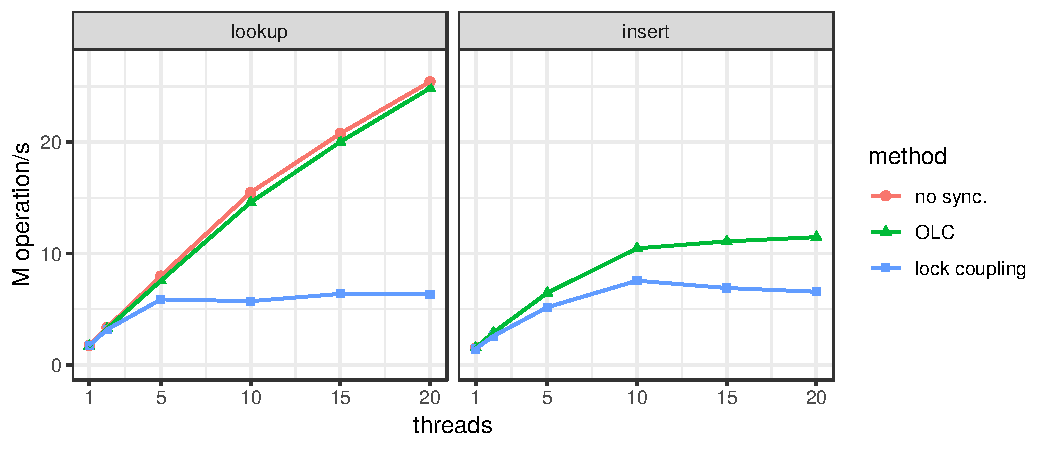
\includegraphics[width=\linewidth]{scale.pdf}
  \vspace{0.2cm}
  \caption{Scalability on 10-core system for B-tree operations (100M values).}
  \label{fig:scale}
\end{figure}

As Figure~\ref{fig:scale} shows, the results change dramatically once we use multiple threads.
For lookup, the scalability of OLC is near-linear up to 20 threads, even though the system has only 10 ``real cores''.
The OLC scalability for insert is also respectable (though not quite as linear because multi-threaded insertion approaches the memory bandwidth of our processor).
The figure also shows that the results of traditional lock coupling with read/write locks are significantly worse than OLC.
With 20 threads, lookup with OLC is 3.9$\times$ faster than traditional lock coupling.

\section{Summary}\label{sec:conc}

Optimistic Lock Coupling (OLC) is an effective synchronization method that combines the simplicity of traditional lock coupling with the superior scalability of lock-free approaches.
OLC is widely applicable and has already been successfully used to synchronize several data structures, including B-trees, binary search trees, and different trie variants.
These features make it highly attractive for modern database systems as well as performance-critical systems software in general.

\begin{thebibliography}{10}

\bibitem{DBLP:conf/spaa/BalmauGHZ16}
O.~Balmau, R.~Guerraoui, M.~Herlihy, and I.~Zablotchi.
\newblock Fast and robust memory reclamation for concurrent data structures.
\newblock In {\em SPAA}, 2016.

\bibitem{DBLP:journals/acta/BayerS77}
R.~Bayer and M.~Schkolnick.
\newblock Concurrency of operations on {B}-trees.
\newblock {\em Acta Informatica}, 9, 1977.

\bibitem{hot}
R.~Binna, E.~Zangerle, M.~Pichl, G.~Specht, and V.~Leis.
\newblock {HOT}: A height optimized trie index for main-memory database
  systems.
\newblock In {\em SIGMOD}, 2018.

\bibitem{DBLP:conf/ppopp/BronsonCCO10}
N.~G. Bronson, J.~Casper, H.~Chafi, and K.~Olukotun.
\newblock A practical concurrent binary search tree.
\newblock In {\em PPOPP}, 2010.

\bibitem{DBLP:conf/vldb/ChaHKK01}
S.~K. Cha, S.~Hwang, K.~Kim, and K.~Kwon.
\newblock Cache-conscious concurrency control of main-memory indexes on
  shared-memory multiprocessor systems.
\newblock In {\em VLDB}, 2001.

\bibitem{intel}
I.~Cutress.
\newblock {Intel} goes for 48-cores: {Cascade-AP} with multi-chip package
  coming soon.
\newblock
  \url{https://www.anandtech.com/show/13535/intel-goes-for-48cores-cascade-ap},
  2018 (accessed January, 2019).

\bibitem{DBLP:conf/cidr/FaleiroA17}
J.~M. Faleiro and D.~J. Abadi.
\newblock Latch-free synchronization in database systems: Silver bullet or
  fool's gold?
\newblock In {\em CIDR}, 2017.

\bibitem{DBLP:journals/ftdb/Graefe11}
G.~Graefe.
\newblock Modern {B}-tree techniques.
\newblock {\em Foundations and Trends in Databases}, 3(4), 2011.

\bibitem{DBLP:conf/hpca/KarnagelDRLLSL14}
T.~Karnagel, R.~Dementiev, R.~Rajwar, K.~Lai, T.~Legler, B.~Schlegel, and
  W.~Lehner.
\newblock Improving in-memory database index performance with
  {Intel}\({}^{\mbox{{\textregistered}}}\) transactional synchronization
  extensions.
\newblock In {\em HPCA}, 2014.

\bibitem{DBLP:journals/tods/LehmanY81}
P.~L. Lehman and S.~B. Yao.
\newblock Efficient locking for concurrent operations on {B}-trees.
\newblock {\em {ACM} Trans. Database Syst.}, 6(4), 1981.

\bibitem{leanstore}
V.~Leis, M.~Haubenschild, A.~Kemper, and T.~Neumann.
\newblock Leanstore: In-memory data management beyond main memory.
\newblock In {\em ICDE}, 2018.

\bibitem{art}
V.~Leis, A.~Kemper, and T.~Neumann.
\newblock The adaptive radix tree: {ARTful} indexing for main-memory databases.
\newblock In {\em ICDE}, 2013.

\bibitem{htmtkde}
V.~Leis, A.~Kemper, and T.~Neumann.
\newblock Scaling {HTM}-supported database transactions to many cores.
\newblock {\em {IEEE} Trans. Knowl. Data Eng.}, 28(2), 2016.

\bibitem{artsync}
V.~Leis, F.~Scheibner, A.~Kemper, and T.~Neumann.
\newblock The {ART} of practical synchronization.
\newblock In {\em DaMoN}, 2016.

\bibitem{DBLP:conf/icde/LevandoskiLS13a}
J.~J. Levandoski, D.~B. Lomet, and S.~Sengupta.
\newblock The {Bw}-tree: A {B}-tree for new hardware platforms.
\newblock In {\em ICDE}, 2013.

\bibitem{DBLP:journals/pvldb/MakreshanskiLS15}
D.~Makreshanski, J.~J. Levandoski, and R.~Stutsman.
\newblock To lock, swap, or elide: On the interplay of hardware transactional
  memory and lock-free indexing.
\newblock {\em {PVLDB}}, 8(11), 2015.

\bibitem{DBLP:dblp_conf/eurosys/MaoKM12}
Y.~Mao, E.~Kohler, and R.~T. Morris.
\newblock Cache craftiness for fast multicore key-value storage.
\newblock In {\em EuroSys}, 2012.

\bibitem{DBLP:journals/tpds/Michael04}
M.~M. Michael.
\newblock Hazard pointers: Safe memory reclamation for lock-free objects.
\newblock {\em {IEEE} Trans. Parallel Distrib. Syst.}, 15(6), 2004.

\bibitem{DBLP:journals/jacm/ShalevS06}
O.~Shalev and N.~Shavit.
\newblock Split-ordered lists: Lock-free extensible hash tables.
\newblock {\em J. {ACM}}, 53(3), 2006.

\bibitem{amd}
A.~Shilov.
\newblock {AMD} previews {EPYC} ‘{Rome}’ processor: Up to 64 {Zen} 2 cores.
\newblock
  \url{https://www.anandtech.com/show/13561/amd-previews-epyc-rome-processor-up-to-64-zen-2-cores},
  2018 (accessed January, 2019).

\bibitem{DBLP:conf/sosp/TuZKLM13}
S.~Tu, W.~Zheng, E.~Kohler, B.~Liskov, and S.~Madden.
\newblock Speedy transactions in multicore in-memory databases.
\newblock In {\em SOSP}, 2013.

\bibitem{buzzword}
Z.~Wang, A.~Pavlo, H.~Lim, V.~Leis, H.~Zhang, M.~Kaminsky, and D.~Andersen.
\newblock Building a {Bw}-tree takes more than just buzz words.
\newblock In {\em SIGMOD}, 2018.

\end{thebibliography}


%\bibliographystyle{abbrv}
%\bibliography{main}

\end{document}

\end{article}


\begin{article}
{Report from the Workshop on Common Model Infrastructure, {ACM KDD 2018}}
{Chaitanya Baru}
\pdfminorversion=5
\documentclass[11pt]{article}
\usepackage{deauthor,times,graphicx,caption,microtype}
\usepackage{hyperref}
\usepackage{listings}
\usepackage{booktabs}

\begin{document}

\title{Optimistic Lock Coupling: A Scalable and Efficient General-Purpose Synchronization Method}

\author{Viktor Leis, Michael Haubenschild\raisebox{0.9ex}{$\ast$}, Thomas Neumann\\ Technische Universit{\"a}t M{\"u}nchen \hspace{0.7cm} Tableau Software\raisebox{0.9ex}{$\ast$} \\ {\{leis,neumann\}{@}in.tum.de} \hspace{0.7cm} {mhaubenschild{@}tableau.com\raisebox{0.9ex}{$\ast$}}}

\maketitle

\begin{abstract}
As the number of cores on commodity processors continues to increase, scalability becomes more and more crucial for overall performance.
Scalable and efficient concurrent data structures are particularly important, as these are often the building blocks of parallel algorithms.
Unfortunately, traditional synchronization techniques based on fine-grained locking have been shown to be unscalable on modern multi-core CPUs.
Lock-free data structures, on the other hand, are extremely difficult to design and often incur significant overhead.

In this work, we make the case for Optimistic Lock Coupling as a practical alternative to both traditional locking and the lock-free approach.
We show that Optimistic Lock Coupling is highly scalable and almost as simple to implement as traditional lock coupling.
Another important advantage is that it is easily applicable to most tree-like data structures.
We therefore argue that Optimistic Lock Coupling, rather than a complex and error-prone custom synchronization protocol, should be the default choice for performance-critical data structures.
\end{abstract}

\section{Introduction}

% more and more cores
Today, Intel's commodity server processors have up to 28 cores and its upcoming microarchitecture will have up to 48 cores per socket~\cite{intel}.
Similarly, AMD currently stands at 32 cores and this number is expected to double in the next generation~\cite{amd}.
Since both platforms support simultaneous multithreading (also known as hyperthreading), affordable commodity servers (with up to two sockets) will soon routinely have between 100 and 200 hardware threads.

% data structure scalability is important
With such a high degree of hardware parallelism, efficient data processing crucially depends on how well concurrent data structures scale.
Internally, database systems use a plethora of data structures like table heaps, internal work queues, and, most importantly, index structures.
Any of these can easily become a scalability (and therefore overall performance) bottleneck on many-core CPUs.

% traditional synchronization: fine-grained locks, slow, cache invalidation
Traditionally, database systems synchronize internal data structures using fine-grained reader/writer locks\footnote{In this work, we focus on data structure synchronization rather than high-level transaction semantics and therefore use the term {\em lock} for what would typically be called {\em latch} in the database literature. We thus follow common computer science (rather than database) terminology.}.
Unfortunately, while fine-grained locking makes lock contention unlikely, it still results in bad scalability because lock acquisition and release require writing to shared memory.
Due to the way cache coherency is implemented on modern multi-core CPUs, these writes cause additional cache misses\footnote{The cache coherency protocol ensures that all copies of a cache line on other cores are invalidated before the write can proceed.} and the cache line containing the lock's internal data becomes a point of physical contention.
As a result, any frequently-accessed lock (e.g., the lock of the root node of a B-tree) severely limits scalability.

% lock-free bw-tree: no more latches, but indirections, extremely complex
Lock-free data structures like the Bw-tree~\cite{DBLP:conf/icde/LevandoskiLS13a} (a lock-free B-tree variant) or the Split-Ordered List~\cite{DBLP:journals/jacm/ShalevS06} (a lock-free hash table) do not acquire any locks and therefore generally scale much better than locking-based approaches (in particular for read-mostly workloads).
However, lock-free synchronization has other downsides:
First, it is very difficult and results in extremely complex and error-prone code (when compared to locking).
Second, because the functionality of atomic primitives provided by the hardware (e.g., atomically compare-and-swap 8 bytes) is limited, complex operations require additional indirections within the data structure.
For example, the Bw-tree requires an indirection table and the Split-Ordered List requires ``dummy nodes'', resulting in overhead due to additional cache misses.

% OLC for the win
In this paper we make the case for {\em Optimistic Lock Coupling (OLC)}, a synchronization method that combines some of the best properties of lock-based and lock-free synchronization.
OLC utilizes a special lock type that can be used in two modes:
The first mode is similar to a traditional mutex and excludes other threads by physically acquiring the underlying lock.
In the second mode, reads can proceed optimistically by validating a version counter that is embedded in the lock (similar to optimistic concurrency control).
The first mode is typically used by writers and the second mode by readers.
Besides this special lock type, OLC is based on the observation that optimistic lock validations can be interleaved/coupled---similar to the pair-wise interleaved lock acquisition of traditional lock coupling.
Hence, the name Optimistic Lock Coupling.

OLC has a number of desirable features:
\begin{itemize}
\item By reducing the number of writes to shared memory locations and thereby avoiding cache invalidations, it {\bf scales well} for most workloads.
\item In comparison to unsynchronized code, it requires few additional CPU instructions making it {\bf efficient}.
\item OLC is {\bf widely applicable} to different data structures. It has already been successfully used for synchronizing binary search trees~\cite{DBLP:conf/ppopp/BronsonCCO10}, tries~\cite{artsync}, trie/B-tree hybrids~\cite{DBLP:dblp_conf/eurosys/MaoKM12}, and B-trees~\cite{buzzword}.
\item In comparison to the lock-free paradigm, it is also {\bf easy to use} and requires few modifications to existing, single-threaded data structures.
\end{itemize}
Despite these positive features and its simplicity, OLC is not yet widely known.
The goal of this paper is therefore to popularize this simple idea and to make a case for it.
We argue that OLC deserves to be widely known.
It is a good default synchronization paradigm---more complex, data structure-specific protocols are seldom beneficial.

The rest of the paper is organized as follows.
Section~\ref{sec:related} discusses related work, tracing the history of OLC and its underlying ideas in the literature.
The core of the paper is Section~\ref{sec:olc}, which describes the ideas behind OLC and how it can be used to synchronize complex data structures.
In Section~\ref{sec:evaluation} we experimentally show that OLC has low overhead and scales well when used to synchronize an in-memory B-tree.
We summarize the paper in Section~\ref{sec:conc}.

\newpage
\section{Related Work}\label{sec:related}

Lock coupling has been proposed as a method for allowing concurrent operations on B-trees in 1977~\cite{DBLP:journals/acta/BayerS77}.
This traditional and still widely-used method, described in detail in Graefe's B-tree survey~\cite{DBLP:journals/ftdb/Graefe11}, is also called ``latch coupling'', ``hand-over-hand locking'', and ``crabbing''.
Because at most two locks are held at-a-time during tree traversal, this technique seemingly allows for a high degree of parallelism---in particular if read/write locks are used to enable inner nodes to be locked in shared mode.
However, as we show in Section~\ref{sec:evaluation}, on modern hardware lock acquisition (even in shared mode) results in suboptimal scalability.

An early alternative from 1981 is a B-tree variant called B-link tree~\cite{DBLP:journals/tods/LehmanY81}, which only holds a single lock at a time.
It is based on the observation that between the release of the parent lock and the acquisition of the child lock, the only ``dangerous'' thing that could have happened is the split of a child node (assuming one does not implement merge operations).
Thus, when a split happens, the key being searched might end up on a neighboring node to the right of the current child node.
A B-link tree traversal therefore detects this condition and, if needed, transparently proceeds to the neighboring node.
Releasing the parent lock early is highly beneficial when the child node needs to be fetched from disk.
For in-memory workloads, however, the B-link tree has the same scalability issues as lock coupling (it acquires just as many locks).

The next major advance, Optimistic Latch-Free Index Traversal (OLFIT)~\cite{DBLP:conf/vldb/ChaHKK01}, was proposed in 2001.
OLFIT introduced the idea of a combined lock/update counter, which we call {\em optimistic lock}. % , for lack of a better name,
Based on these per-node optimistic locks and the synchronization protocol of the B-link tree, OLFIT finally achieves good scalability on parallel processors.
The OLFIT protocol is fairly complex, as it requires both the non-trivial B-link protocol and optimistic locks.
Furthermore, like the B-link tree protocol, it does not support merging nodes, and is specific to B-trees (cannot easily be applied to other data structures).

In the following two decades, the growth of main-memory capacity led to much research into other data structures besides the venerable B-tree.
Particularly relevant for our discussion is Bronson et al.'s~\cite{DBLP:conf/ppopp/BronsonCCO10} concurrent binary search tree, which is based on optimistic version validation and has a sophisticated, data structure-specific synchronization protocol.
To the best of our knowledge, this 2010 paper is the first that, as part of its protocol, interleaves version validation across nodes---rather than validating each node separately like OLFIT.
In that paper, this idea is called ``hand-over-hand, optimistic validation'', while we prefer the term Optimistic Lock Coupling to highlight the close resemblance to traditional lock coupling.
Similarly, Mao et al.'s~\cite{DBLP:dblp_conf/eurosys/MaoKM12} Masstree (a concurrent hybrid trie/B-tree) is also based on the same ideas, but again uses them as part of a more complex protocol.

The Adaptive Radix Tree (ART)~\cite{art} is another recent in-memory data structure, which we proposed in 2013.
In contrast to the two data structures just mentioned, it was originally designed with single-threaded performance in mind without supporting concurrency.
To add support for concurrency, we initially started designing a custom protocol called Read-Optimized Write Exclusion (ROWEX)~\cite{artsync}, which turned out to be non-trivial and requires modifications of the underlying data structure\footnote{Note that ROWEX is already easier to apply to existing data structures than the lock-free approach. The difficulty depends on the data structure. Applying ROWEX is hard for B-trees with sorted keys and fairly easy for copy-on-write data structures like the Height Optimized Trie~\cite{hot}---with ART being somewhere in the middle.}.
However, fairly late in the project, we also realized, that OLC {\em alone} (rather than as part of a more complex protocol) is sufficient to synchronize ART.
No other changes to the data structure were necessary.
Both approaches were published and experimentally evaluated in a followup paper~\cite{artsync}, which shows that, despite its simplicity, OLC is efficient, scalable, and generally outperforms ROWEX.

Similar results were recently published regarding B-trees~\cite{buzzword}.
In this experimental study a simple OLC-based synchronization outperformed the Bw-tree~\cite{DBLP:conf/icde/LevandoskiLS13a}, a complex lock-free synchronization approach.
Another recent paper shows that for write-intensive workloads, locking often performs better than lock-free synchronization~\cite{DBLP:conf/cidr/FaleiroA17}.
These experiences indicate that OLC is a general-purpose synchronization paradigm and motivate the current paper.

%foster b-tree\cite{DBLP:journals/tods/GraefeKK12}
%Shasha theory~\cite{DBLP:journals/tods/ShashaG88}

\section{Optimistic Lock Coupling}\label{sec:olc}

% locks suck
The standard technique for inter-thread synchronization is mutual exclusion using fine-grained locks.
In a B-tree, for example, every node usually has its own associated lock, which is acquired before accessing that node.
The problem of locking on modern multi- and many-core processors is that lock acquisition and release require writing to the shared memory location that implements the lock.
This write causes exclusive ownership of the underlying cache line and invalidates copies of it on all other processor cores.
For hierarchical, tree-like data structures, the lock of the root node becomes a point of physical contention---even in read-only workloads and even when read/write locks are used.
Depending on the specific data structure, number of cores, cache coherency protocol implementation, cache topology, whether Non-Uniform Memory Access (NUMA) is used, locking can even result in multi-threaded performance that is worse than single-threaded execution.

% in b-trees this happens very much
The inherent pessimism of locking is particularly unfortunate for B-trees:
Despite the fact that logical modifications of the root node are very infrequent, every B-tree operation must lock the root node during tree traversal\footnote{To a lesser extent this obviously applies to all inner nodes, not just the root.}.
Even the vast majority of update operations (with the exception of splits and merges), only modify a single leaf node.
These observations indicate that a more optimistic approach, which does not require locking inner nodes, would be very beneficial for B-trees.

\subsection{Optimistic Locks}

% optimism to the rescue
As the name indicates, optimistic locks try to solve the scalability issues of traditional locks using an optimistic approach.
Instead of always physically acquiring locks, even for nodes that are unlikely to be modified simultaneously, after-the-fact validation is used to detect conflicts.
This is done by augmenting each lock with a version/update counter that is incremented on every modification.
Using this version counter, readers can optimistically proceed before validating that the version did not change to ensure that the read was safe.
If validation fails, the operation is restarted.

% details on opt locks
Using optimistic locks, a read-only node access (i.e., the majority of all operations in a B-tree) does not acquire the lock and does not increment the version counter.
Instead, it performs the following steps:
\begin{enumerate}
\item read lock version (restart if lock is not free)
\item access node
\item read the version again and validate that it has not changed in the meantime
\end{enumerate}
If the last step (the validation) fails, the operation has to be restarted.
Write operations, on the other hand, are more similar to traditional locking:
\begin{enumerate}
\item acquire lock (wait if necessary)
\item access/write to node
\item increment version and unlock node
\end{enumerate}
Writes can therefore protect a node from other writes.

% similar to locks
As we observed in an earlier paper~\cite{artsync}, because of similar semantics, optimistic locks can be hidden behind an API very similar to traditional read/write locks.
Both approaches have an exclusive lock mode, and acquiring a traditional lock in shared mode is analogous to optimistic version validation.
Furthermore, like with some implementations of traditional read/write locks, optimistic locks allow upgrading a shared lock to an exclusive lock.
Lock upgrades are, for example, used to avoid most B-tree update operations from having to lock inner nodes.
In our experience, the close resemblance of optimistic and traditional locks simplifies the reasoning about optimistic locks;
one can apply similar thinking as in traditional lock-based protocols.

\subsection{Lock Coupling with Optimistic Locks}

\begin{figure}
  \centering
  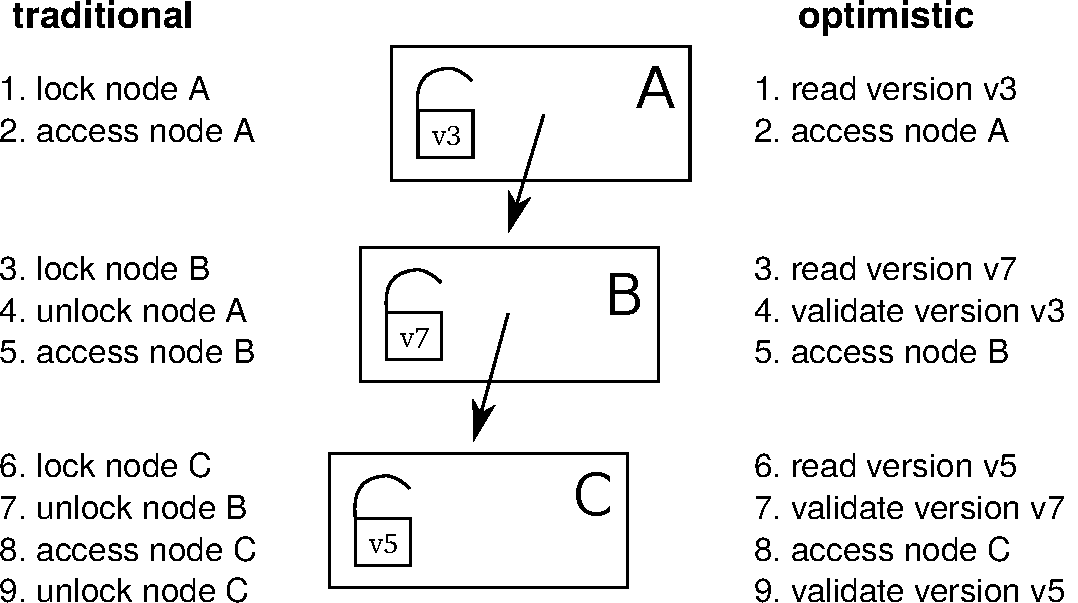
\includegraphics[width=0.65\linewidth]{olcall.pdf}
  \vspace{0.2cm}
  \caption{Comparison of a lookup operation in a 3-level tree using traditional lock coupling (left-hand side) vs.~optimistic lock coupling (right-hand side).}
  \label{fig:olc}
\end{figure}

The traditional and most common lock-based synchronization protocol for B-trees is lock coupling, which interleaves lock acquisitions while holding at most two locks at a time.
If, as we observed earlier, optimistic locks have similar semantics as traditional locks, it is natural to ask whether lock coupling can be combined with optimistic locks.
And indeed the answer is yes: One can almost mechanically translate traditional lock coupling code to optimistic lock coupling code.
This is illustrated in Figure~\ref{fig:olc}, which compares the traversal in a tree of height 3 using traditional and optimistic locks.
As the figure shows, the main difference is that locking is translated to reading the version and that unlocking becomes validation of the previously read version.
This simple change provides efficient lock-free tree traversal without the need to design a complex synchronization protocol.

It is important to emphasize the conceptual simplicity of OLC in comparison to data structures that use custom protocols like the Bw-tree~\cite{DBLP:conf/icde/LevandoskiLS13a}.
To implement lock-free access, the Bw-tree requires an indirection table, delta nodes, complex splitting and merging logic, retry logic, etc.
OLC, on the other hand, can directly be applied to B-trees mostly by adding the appropriate optimistic locking code and without modifying the node layout itself.
Therefore, OpenBw-Tree, an open source implementation of the Bw-tree, requires an order of magnitude more code than a B-tree based on OLC\footnote{Both implementations are available on GitHub: \url{https://github.com/wangziqi2016/index-microbench}}.
Given how difficult it is to develop, validate, and debug lock-free code, simplicity is obviously a major advantage.

\subsection{Correctness Aspects}

\begin{figure}
  % \centering
  %[basicstyle=\normalsize\ttfamily,showstringspaces=false,columns=fullflexible,breaklines=false,breakatwhitespace=true,numbers=none,numberstyle=\small,style=C,keepspaces=true]
\begin{lstlisting}[basicstyle=\ttfamily,language=C++,numbers=left,numberstyle=\small]
std::atomic<BTreeNode*> root;

// search for key in B+tree, returns payload in resultOut
bool lookup(Key key, Value& resultOut) {
   BTreeNode* node = root.load();
   uint64_t nodeVersion = node->readLockOrRestart();
   if (node != root.load()) // make sure the root is still the root
      restart();

   BTreeInner<Key>* parent = nullptr;
   uint64_t parentVersion = 0;

   while (node->isInner()) {
      auto inner = (BTreeInner*)node;

      // unlock parent and make current node the parent
      if (parent)
         parent->readUnlockOrRestart(parentVersion);
      parent = inner;
      parentVersion = nodeVersion;

      // search for next node
      node = inner->findChild(key);
      // validate 'inner' to ensure that 'node' pointer is valid
      inner->checkOrRestart(nodeVersion);
      // now it safe to dereference 'node' pointer (read its version)
      nodeVersion = node->readLockOrRestart();
   }

   // search in leaf and retrieve payload
   auto leaf = (BTreeLeaf*)node;
   bool success = leaf->findValue(key, resultOut);

   // unlock everything
   if (parent)
      parent->readUnlockOrRestart(parentVersion);
   node->readUnlockOrRestart(nodeVersion);

   return success;
}
\end{lstlisting}
  \vspace{0.2cm}
  \caption{B-tree lookup code using OLC. For simplicity, the restart logic is not shown.}
  \label{fig:lookup}
\end{figure}

So far, we have introduced the high-level ideas behind OLC and have stressed its similarity to traditional lock coupling.
Let us now discuss some cases where the close similarity between lock coupling and OLC breaks down.
To make this more concrete, we show the B-tree lookup code in Figure~\ref{fig:lookup}.
In the code, \texttt{readLockOrRestart} reads the lock version and \texttt{readUnlockOrRestart} validates that the read was correct.

One issue with OLC is that any pointer speculatively read from a node may point to invalid memory (if that node is modified concurrently).
Dereferencing such a pointer (e.g., to read its optimistic lock), may cause a segmentation fault or undefined behavior.
In the code shown in Figure~\ref{fig:lookup}, this problem is prevented by the extra check in line 25, which ensures that the read from the node containing the pointer was correct.
Without this additional validation, the code would in line 27 dereference the pointer speculatively read in line 23.
Note that the implementation of \texttt{checkOrRestart} is actually identical to \texttt{readUnlockOrRestart}.
We chose to give it a different name to highlight the fact that this extra check would not be necessary with read/write locks.

Another potential issue with optimistic locks is code that does not terminate.
Code that speculatively accesses a node, like an intra-node binary search, should be written in a way such that it always terminates---even in the presence of concurrent writes.
Otherwise, the validation code that detects the concurrent write will never run.
The binary search of a B-tree, for example, needs to be written in such a way that each comparison makes progress.
For some data structures that do not require loops in the traversal code (like ART) termination is trivially true.

\subsection{Implementation Details}

% implementation, efficiency
To implement an optimistic lock, one can combine the lock and the version counter into a single 64-bit\footnote{Even after subtracting one bit for the lock status, a back-of-the-envelope calculation can show that 63 bits are large enough to never overflow in practice.} word~\cite{artsync}.
A typical read operation will therefore merely consist of reading this version counter atomically.
In C++11 this can be implemented using the \texttt{std::atomic} type.

On x86, atomic reads are cheap because of x86's strong memory order guarantees.
No memory fences are required for sequentially-consistent loads, which are translated (by both GCC and clang) into standard \texttt{MOV} instructions.
Hence, the only effect of \texttt{std::atomic} for loads is preventing instruction re-ordering.
This makes version access and validation cheap.
Acquiring and releasing an optimistic lock in exclusive mode has comparable cost to a traditional lock:
A fairly expensive sequentially-consistent store is needed for acquiring a lock, while a standard \texttt{MOV} suffices for releasing it.
A simple sinlock-based implementation of optimistic locks can be found in the appendix of an earlier paper~\cite{artsync}.

OLC code must be able to handle restarts since validation or lock upgrade can fail due to concurrent writers.
Restarts can easily be implemented by wrapping the data structure operation in a loop (for simplicity not shown in Figure~\ref{fig:lookup}).
Such a loop also enables limiting the number of optimistic retry operations and falling back to pessimistic locking in cases of very heavy contention.
The ability to fall back to traditional locking is a major advantage of OLC in terms of robustness over lock-free approaches, which do not have this option.

In addition to the optimistic shared mode and the exclusive mode, optimistic locks also support a ``shared pessimistic'' mode, which physically acquires the lock in shared mode (allowing multiple concurrent readers but no writers).
This mode is useful for table (or range) scans that touch many tuples on a leaf page (which would otherwise easily abort).
Finally, let us mention that large range scans and table scans, should be broken up into several per-node traversals as is done in the LeanStore~\cite{leanstore} system.

Like all lock-free data structures, but unlike traditional locking and Hardware Transactional Memory~\cite{DBLP:conf/hpca/KarnagelDRLLSL14,DBLP:journals/pvldb/MakreshanskiLS15,htmtkde}, OLC requires care when deleting (and reusing) nodes.
The reason is that a deleting thread can never be sure that a node can be reclaimed because other threads might still be optimistically reading from that node.
Therefore, standard solutions like epoch-based reclamation~\cite{DBLP:conf/sosp/TuZKLM13}, hazard pointers~\cite{DBLP:journals/tpds/Michael04}, or optimized hazard pointers~\cite{DBLP:conf/spaa/BalmauGHZ16} need to be used.
These memory reclamation techniques are, however, largely orthogonal to the synchronization protocol itself.

%-lock-free is not a strong guarantee

\newpage
\section{Evaluation}\label{sec:evaluation}

Let us now experimentally evaluate the overhead and scalability of OLC.
For the experiments, we use an in-memory B+tree implemented in C++11 using templates, which is configured to use nodes of 4096 bytes, random 8 byte keys, and 8 byte payloads.
Based on this B-tree, we compare the following synchronization approaches:
\begin{itemize}
\item an OLC implementation\footnote{An almost identical OLC implementation is available on github: \url{https://github.com/wangziqi2016/index-microbench/tree/master/BTreeOLC}}
\item a variant based on traditional lock coupling and read/write locks
\item the unsynchronized B-tree, which obviously is only correct for read-only workloads but allows measuring the overhead of synchronization
\end{itemize}
Note that earlier work has compared the OLC implementation with a Bw-tree implementation~\cite{buzzword} and other state-of-the-art in-memory index structures.

We use a Haswell EP system with an Intel Xeon E5-2687W v3 CPU, which has 10 cores (20 ``Hyper-Threads'') and 25~MB of L3 cache.
The system is running Ubuntu 18.10 and we use GCC 8.2.0 to compile our code.
The CPU counters are obtained using the Linux perf API\footnote{We use the following convenience wrapper: \url{https://github.com/viktorleis/perfevent}}.

\begin{table}
  \caption{Performance and CPU counters for lookup and insert operations in a B-tree with 100M keys. We perform 100M operations and normalize the CPU counters by that number.}
  \label{tab:overhead}
  \centering
  \begin{tabular}{lrrrrrrr}\toprule
                    &         &        &        & instruc-  & L1     & L3     & branch \\
                    & threads & M op/s & cycles & tions & misses & misses & misses \\\midrule
lookup (no sync.)   & 1       & 1.72   & 2028   & 283     & 39.1   & 14.9   & 16.1   \\
lookup (OLC)        & 1       & 1.65   & 2107   & 370     & 43.9   & 15.1   & 16.7   \\
lookup (lock coup.) & 1       & 1.72   & 2078   & 365     & 42.3   & 16.9   & 15.7   \\\midrule
insert (no sync.)   & 1       & 1.51   & 2286   & 530     & 59.8   & 31.1   & 17.3   \\
insert (OLC)        & 1       & 1.50   & 2303   & 629     & 61.2   & 31.1   & 16.5   \\
insert (lock coup.) & 1       & 1.41   & 2473   & 644     & 61.0   & 31.0   & 17.2   \\\midrule
lookup (no sync.)   & 10      & 15.48  & 2058   & 283     & 38.6   & 15.5   & 16.0   \\
lookup (OLC)        & 10      & 14.60  & 2187   & 370     & 43.8   & 15.8   & 16.8   \\
lookup (lock coup.) & 10      & 5.71   & 5591   & 379     & 54.2   & 17.0   & 14.8   \\\midrule
insert (no sync.)   & 10      & -      & -      & -       & -      & -      & -      \\
insert (OLC)        & 10      & 10.46  & 2940   & 656     & 62.0   & 32.5   & 16.8   \\
insert (lock coup.) & 10      & 7.55   & 4161   & 667     & 75.0   & 28.6   & 16.2   \\
    \bottomrule
\end{tabular}
\end{table}

Table~\ref{tab:overhead} compares the performance and CPU counters for lookup and insert operations in a B-tree with 100M keys.
With {\em single-threaded} execution, we observe that all three approaches have very similar performance.
Adding traditional or optimistic locks to unsynchronized B-tree code results in up to 30\% of additional instructions without affecting single-threaded performance much.

\begin{figure}
  \centering
  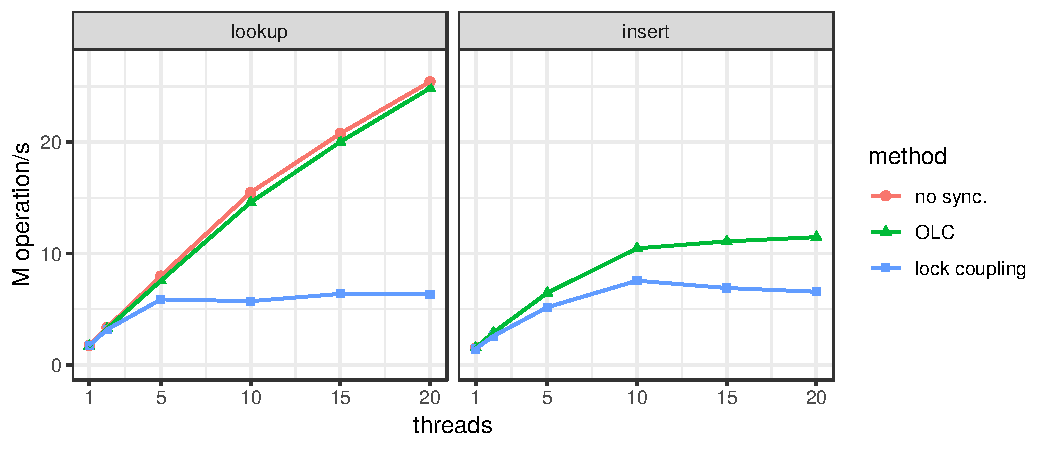
\includegraphics[width=\linewidth]{scale.pdf}
  \vspace{0.2cm}
  \caption{Scalability on 10-core system for B-tree operations (100M values).}
  \label{fig:scale}
\end{figure}

As Figure~\ref{fig:scale} shows, the results change dramatically once we use multiple threads.
For lookup, the scalability of OLC is near-linear up to 20 threads, even though the system has only 10 ``real cores''.
The OLC scalability for insert is also respectable (though not quite as linear because multi-threaded insertion approaches the memory bandwidth of our processor).
The figure also shows that the results of traditional lock coupling with read/write locks are significantly worse than OLC.
With 20 threads, lookup with OLC is 3.9$\times$ faster than traditional lock coupling.

\section{Summary}\label{sec:conc}

Optimistic Lock Coupling (OLC) is an effective synchronization method that combines the simplicity of traditional lock coupling with the superior scalability of lock-free approaches.
OLC is widely applicable and has already been successfully used to synchronize several data structures, including B-trees, binary search trees, and different trie variants.
These features make it highly attractive for modern database systems as well as performance-critical systems software in general.

\begin{thebibliography}{10}

\bibitem{DBLP:conf/spaa/BalmauGHZ16}
O.~Balmau, R.~Guerraoui, M.~Herlihy, and I.~Zablotchi.
\newblock Fast and robust memory reclamation for concurrent data structures.
\newblock In {\em SPAA}, 2016.

\bibitem{DBLP:journals/acta/BayerS77}
R.~Bayer and M.~Schkolnick.
\newblock Concurrency of operations on {B}-trees.
\newblock {\em Acta Informatica}, 9, 1977.

\bibitem{hot}
R.~Binna, E.~Zangerle, M.~Pichl, G.~Specht, and V.~Leis.
\newblock {HOT}: A height optimized trie index for main-memory database
  systems.
\newblock In {\em SIGMOD}, 2018.

\bibitem{DBLP:conf/ppopp/BronsonCCO10}
N.~G. Bronson, J.~Casper, H.~Chafi, and K.~Olukotun.
\newblock A practical concurrent binary search tree.
\newblock In {\em PPOPP}, 2010.

\bibitem{DBLP:conf/vldb/ChaHKK01}
S.~K. Cha, S.~Hwang, K.~Kim, and K.~Kwon.
\newblock Cache-conscious concurrency control of main-memory indexes on
  shared-memory multiprocessor systems.
\newblock In {\em VLDB}, 2001.

\bibitem{intel}
I.~Cutress.
\newblock {Intel} goes for 48-cores: {Cascade-AP} with multi-chip package
  coming soon.
\newblock
  \url{https://www.anandtech.com/show/13535/intel-goes-for-48cores-cascade-ap},
  2018 (accessed January, 2019).

\bibitem{DBLP:conf/cidr/FaleiroA17}
J.~M. Faleiro and D.~J. Abadi.
\newblock Latch-free synchronization in database systems: Silver bullet or
  fool's gold?
\newblock In {\em CIDR}, 2017.

\bibitem{DBLP:journals/ftdb/Graefe11}
G.~Graefe.
\newblock Modern {B}-tree techniques.
\newblock {\em Foundations and Trends in Databases}, 3(4), 2011.

\bibitem{DBLP:conf/hpca/KarnagelDRLLSL14}
T.~Karnagel, R.~Dementiev, R.~Rajwar, K.~Lai, T.~Legler, B.~Schlegel, and
  W.~Lehner.
\newblock Improving in-memory database index performance with
  {Intel}\({}^{\mbox{{\textregistered}}}\) transactional synchronization
  extensions.
\newblock In {\em HPCA}, 2014.

\bibitem{DBLP:journals/tods/LehmanY81}
P.~L. Lehman and S.~B. Yao.
\newblock Efficient locking for concurrent operations on {B}-trees.
\newblock {\em {ACM} Trans. Database Syst.}, 6(4), 1981.

\bibitem{leanstore}
V.~Leis, M.~Haubenschild, A.~Kemper, and T.~Neumann.
\newblock Leanstore: In-memory data management beyond main memory.
\newblock In {\em ICDE}, 2018.

\bibitem{art}
V.~Leis, A.~Kemper, and T.~Neumann.
\newblock The adaptive radix tree: {ARTful} indexing for main-memory databases.
\newblock In {\em ICDE}, 2013.

\bibitem{htmtkde}
V.~Leis, A.~Kemper, and T.~Neumann.
\newblock Scaling {HTM}-supported database transactions to many cores.
\newblock {\em {IEEE} Trans. Knowl. Data Eng.}, 28(2), 2016.

\bibitem{artsync}
V.~Leis, F.~Scheibner, A.~Kemper, and T.~Neumann.
\newblock The {ART} of practical synchronization.
\newblock In {\em DaMoN}, 2016.

\bibitem{DBLP:conf/icde/LevandoskiLS13a}
J.~J. Levandoski, D.~B. Lomet, and S.~Sengupta.
\newblock The {Bw}-tree: A {B}-tree for new hardware platforms.
\newblock In {\em ICDE}, 2013.

\bibitem{DBLP:journals/pvldb/MakreshanskiLS15}
D.~Makreshanski, J.~J. Levandoski, and R.~Stutsman.
\newblock To lock, swap, or elide: On the interplay of hardware transactional
  memory and lock-free indexing.
\newblock {\em {PVLDB}}, 8(11), 2015.

\bibitem{DBLP:dblp_conf/eurosys/MaoKM12}
Y.~Mao, E.~Kohler, and R.~T. Morris.
\newblock Cache craftiness for fast multicore key-value storage.
\newblock In {\em EuroSys}, 2012.

\bibitem{DBLP:journals/tpds/Michael04}
M.~M. Michael.
\newblock Hazard pointers: Safe memory reclamation for lock-free objects.
\newblock {\em {IEEE} Trans. Parallel Distrib. Syst.}, 15(6), 2004.

\bibitem{DBLP:journals/jacm/ShalevS06}
O.~Shalev and N.~Shavit.
\newblock Split-ordered lists: Lock-free extensible hash tables.
\newblock {\em J. {ACM}}, 53(3), 2006.

\bibitem{amd}
A.~Shilov.
\newblock {AMD} previews {EPYC} ‘{Rome}’ processor: Up to 64 {Zen} 2 cores.
\newblock
  \url{https://www.anandtech.com/show/13561/amd-previews-epyc-rome-processor-up-to-64-zen-2-cores},
  2018 (accessed January, 2019).

\bibitem{DBLP:conf/sosp/TuZKLM13}
S.~Tu, W.~Zheng, E.~Kohler, B.~Liskov, and S.~Madden.
\newblock Speedy transactions in multicore in-memory databases.
\newblock In {\em SOSP}, 2013.

\bibitem{buzzword}
Z.~Wang, A.~Pavlo, H.~Lim, V.~Leis, H.~Zhang, M.~Kaminsky, and D.~Andersen.
\newblock Building a {Bw}-tree takes more than just buzz words.
\newblock In {\em SIGMOD}, 2018.

\end{thebibliography}


%\bibliographystyle{abbrv}
%\bibliography{main}

\end{document}

\end{article}


\fi

\end{articlesection}

%\begin{newssection}{TCDE Election}
%
% there will be other letters- and a blank page will appear in your document
% but the special issue part will be fine
%
%\begin{news}{Letter from the Editor-in-Chief}
%{David Lomet}{Microsoft Corporation}
%\documentclass[11pt]{article} 

\usepackage{deauthor,times,graphicx}
%\usepackage{url}
\usepackage{hyperref}

\begin{document}

\subsection*{ICDE 2018}

Repeating my comment from the last issue-

The IEEE International Conference on Data Engineering will be held in April 14-19, 2018 in Paris, France.  This is the flagship conference of the Computer Society's Technical Committee on Data Engineering.  It is a great conference, at a great location.  What could possibly be better than April in Paris at ICDE!  I am attending and hope to see you there.

\subsection*{About the Bulletin}

This March current issue marks the end of editorial tenure for the Bulletin's current set of editors.  So it is once again time for me to pat myself on the back.  This current set, Tim Kraska, Tova Milo, and Haixun Wang, continue my outstanding success (he says modestly) in finding and choosing great editors.  All three have done truly fine jobs at producing issues that bring to our readers surveys of the latest work in very current areas. The success of the Bulletin depends on great issue editors.  I want to thank Tim, Tova, and Haixun for being exactly that with the fine jobs that they have done.  There was unexpected ``scrambling" over the past two years, so I want to thank them also for their flexibility in coping with this.  


\subsection*{The Current Issue}

Don't you get tired of someone shouting ``FAKE NEWS!".  Or perhaps even worse, being exposed to fake news before it has been labeled as such?  Our political conversations seem increasingly to include many variations of ``fake news" and discussions about which news is fake.  ``Sad." So where am I going with this?

The database world has been working on a key aspect of this problem for many years.  The technical area is called ``data provenance".  And it addresses the problem of where information comes from and how it impacts the subsequent processing of data and the reported results.  The June, 2010 issue was the last one on provenance.  And seven years is a long time in an active technical area, especially an area as important as this.

The current issue is focused on the applications of provenance.  Without delving into the current political scene, a reader will clearly see how extensively provenance management can be used.  As we gain more insight into its application scenarios, we also gain more insight into how to manage provenance.  This symbiotic relationship is driving the field forward.   Tova Milo, our Bulletin editor for the issue, has done an excellent job in bringing the issue together, making it a great place to learn about and track progress in the field.  The result is an issue well worth reading.



\end{document}



%\end{news}
%
%\newpage
%
%% your introductory letter goes here
%
%\begin{news}{Letter from the Special Issue Editor}
%{Joseph E. Gonzalez}{University of California at Berkeley\\ Berkeley, CA}
%\graphicspath{{letters/}}
%\documentclass[11pt]{article} 

\usepackage{deauthor,times,graphicx}
%\usepackage{url}
\usepackage{hyperref}



\begin{document}

Machine learning is rapidly maturing into an engineering discipline at the center of a growing range of applications.
This widespread adoption of machine learning techniques poses a new set challenges around the management of the data, code, models, and their relationship throughout the machine learning life-cycle.
In this issue of the Data Engineering Bulletin we have solicited work from both academic and industrial leaders in the data engineering community that are exploring how data engineering techniques can be used to address the challenges of the machine learning life-cycle.




\begin{figure}[h]
\centering
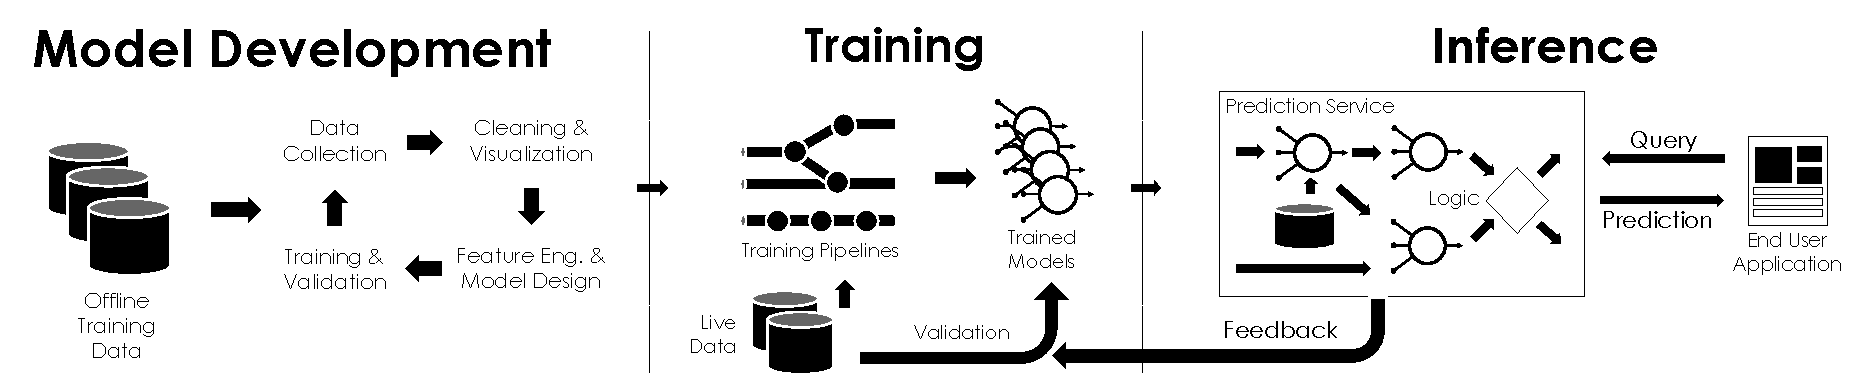
\includegraphics[width=\textwidth]{letters/pipeline.pdf}
\caption{\small \textbf{Machine Learning Life-cycle.} A simplified depiction of the key stages of a machine learning application.}
\label{fig:mllc}
\end{figure}


The machine learning life-cycle (Fig.~\ref{fig:mllc}) spans not only the model development, but also production training and inference.
Each stage demands different skills (e.g., neural network design, data management, and cluster management) and imposes different requirements on the underlying systems.
Yet there is an overwhelming need for unifying design principles and technologies to address pervasive problems including: feature management, data provenance, pipeline reproducibility, low-latency serving, and prediction monitoring just to name a few.


There has been substantial recent progress in systems to aid in managing the machine learning life-cycle.  
Large industrial projects like 
FB Learner Flow 
% \href{https://code.fb.com/core-data/introducing-fblearner-flow-facebook-s-ai-backbone/}{FB Learner Flow}
from Facebook, 
Michelangelo 
% \href{https://eng.uber.com/michelangelo/}{Michelangelo} 
from Uber, and 
TFX 
% \href{https://www.tensorflow.org/tfx/}{TFX} 
from Google have received a considerable of recent attention.  
In this issue we have solicited publications from several more recent industrial and academic projects.

The first paper, by a team at Amazon Research, provides an overview of several real-world use cases and then outlines the key conceptual, data management, and engineering challenges faced in production machine learning systems.
Rather than advocating a single system, this work describes some design principles that can inform potential solutions.


The second and third papers explores the challenges of model management and provenance across the machine learning life-cycle.
They motivate the need for systems to track models and their meta-data to improve reproducibility, collaboration, and governance. 
% expands upon the machine learning life-cycle 
% to include: data preparation, feature engineering, model training, deployment, and maintenance
% and explores the challenges of model 
The second paper introduces, ModelDB, an open-source system for model management and describe some of the functionality and design decisions. 
The third paper describes a related system, ProvDB, that uses a graph data model to capture and query fine-grained versioned lineage of data, scripts, and artifacts throughout the data analysis process.


The fourth paper, by a team at Databricks Inc., describes, MLFlow, a new open-source system to address the challenges of experimentation, reproducibility, and deployment. 
This work leverages containerization to capture the model development environment and a simple tracking API to enable experiment tracking.
The extensible model containerization enables model developers to more easily collaborate around modeling environments and then deploy model containers.


The last paper, by a team at Microsoft, focuses on inference and explores the challenges and opportunities of serving white-box prediction pipelines.  
In contrast to the containerization of pipelines in MLFlow, the Microsoft team leverage knowledge about the internal of the prediction pipeline to more efficient serve predictions. 



\end{document}



%\end{news}


%\end{newssection}

%\begin{newssection}{TCDE Election}

% there will be other letters- and a blank page will appear in your document
% but the special issue part will be fine

%\begin{news}{Letter from the Editor-in-Chief}
%{David Lomet}{Microsoft Corporation}
%\documentclass[11pt]{article} 

\usepackage{deauthor,times,graphicx}
%\usepackage{url}
\usepackage{hyperref}

\begin{document}

\subsection*{ICDE 2018}

Repeating my comment from the last issue-

The IEEE International Conference on Data Engineering will be held in April 14-19, 2018 in Paris, France.  This is the flagship conference of the Computer Society's Technical Committee on Data Engineering.  It is a great conference, at a great location.  What could possibly be better than April in Paris at ICDE!  I am attending and hope to see you there.

\subsection*{About the Bulletin}

This March current issue marks the end of editorial tenure for the Bulletin's current set of editors.  So it is once again time for me to pat myself on the back.  This current set, Tim Kraska, Tova Milo, and Haixun Wang, continue my outstanding success (he says modestly) in finding and choosing great editors.  All three have done truly fine jobs at producing issues that bring to our readers surveys of the latest work in very current areas. The success of the Bulletin depends on great issue editors.  I want to thank Tim, Tova, and Haixun for being exactly that with the fine jobs that they have done.  There was unexpected ``scrambling" over the past two years, so I want to thank them also for their flexibility in coping with this.  


\subsection*{The Current Issue}

Don't you get tired of someone shouting ``FAKE NEWS!".  Or perhaps even worse, being exposed to fake news before it has been labeled as such?  Our political conversations seem increasingly to include many variations of ``fake news" and discussions about which news is fake.  ``Sad." So where am I going with this?

The database world has been working on a key aspect of this problem for many years.  The technical area is called ``data provenance".  And it addresses the problem of where information comes from and how it impacts the subsequent processing of data and the reported results.  The June, 2010 issue was the last one on provenance.  And seven years is a long time in an active technical area, especially an area as important as this.

The current issue is focused on the applications of provenance.  Without delving into the current political scene, a reader will clearly see how extensively provenance management can be used.  As we gain more insight into its application scenarios, we also gain more insight into how to manage provenance.  This symbiotic relationship is driving the field forward.   Tova Milo, our Bulletin editor for the issue, has done an excellent job in bringing the issue together, making it a great place to learn about and track progress in the field.  The result is an issue well worth reading.



\end{document}



%\end{news}
%
%\newpage
%
%% your introductory letter goes here
%
%\begin{news}{Letter from the Special Issue Editor}
%{Joseph E. Gonzalez}{University of California at Berkeley\\ Berkeley, CA}
%\documentclass[11pt]{article} 

\usepackage{deauthor,times,graphicx}
%\usepackage{url}
\usepackage{hyperref}



\begin{document}

Machine learning is rapidly maturing into an engineering discipline at the center of a growing range of applications.
This widespread adoption of machine learning techniques poses a new set challenges around the management of the data, code, models, and their relationship throughout the machine learning life-cycle.
In this issue of the Data Engineering Bulletin we have solicited work from both academic and industrial leaders in the data engineering community that are exploring how data engineering techniques can be used to address the challenges of the machine learning life-cycle.




\begin{figure}[h]
\centering
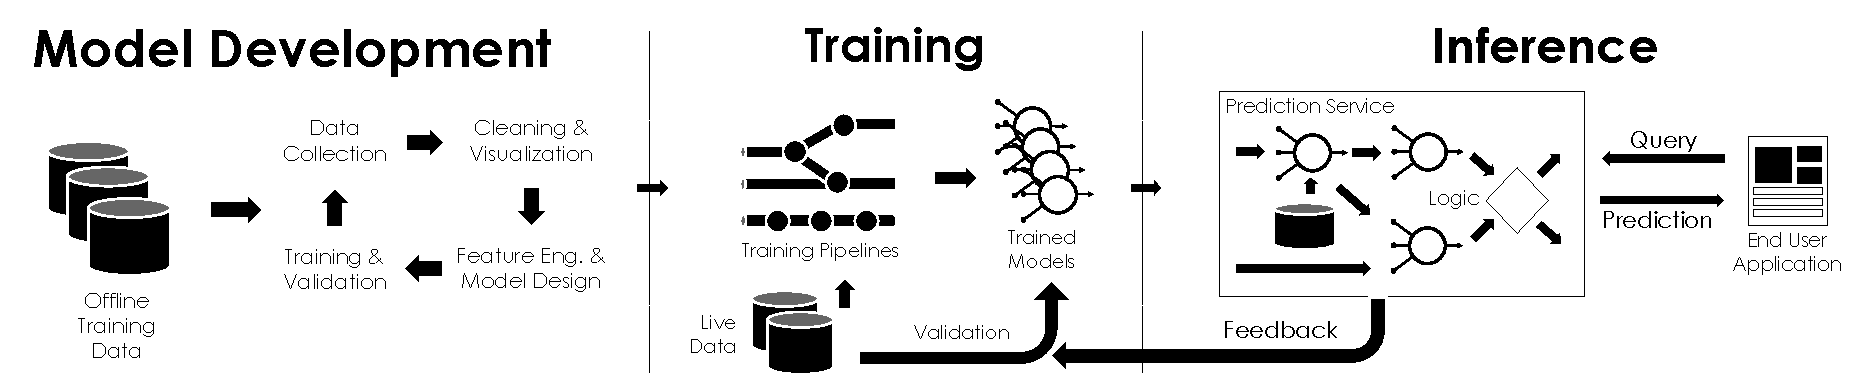
\includegraphics[width=\textwidth]{letters/pipeline.pdf}
\caption{\small \textbf{Machine Learning Life-cycle.} A simplified depiction of the key stages of a machine learning application.}
\label{fig:mllc}
\end{figure}


The machine learning life-cycle (Fig.~\ref{fig:mllc}) spans not only the model development, but also production training and inference.
Each stage demands different skills (e.g., neural network design, data management, and cluster management) and imposes different requirements on the underlying systems.
Yet there is an overwhelming need for unifying design principles and technologies to address pervasive problems including: feature management, data provenance, pipeline reproducibility, low-latency serving, and prediction monitoring just to name a few.


There has been substantial recent progress in systems to aid in managing the machine learning life-cycle.  
Large industrial projects like 
FB Learner Flow 
% \href{https://code.fb.com/core-data/introducing-fblearner-flow-facebook-s-ai-backbone/}{FB Learner Flow}
from Facebook, 
Michelangelo 
% \href{https://eng.uber.com/michelangelo/}{Michelangelo} 
from Uber, and 
TFX 
% \href{https://www.tensorflow.org/tfx/}{TFX} 
from Google have received a considerable of recent attention.  
In this issue we have solicited publications from several more recent industrial and academic projects.

The first paper, by a team at Amazon Research, provides an overview of several real-world use cases and then outlines the key conceptual, data management, and engineering challenges faced in production machine learning systems.
Rather than advocating a single system, this work describes some design principles that can inform potential solutions.


The second and third papers explores the challenges of model management and provenance across the machine learning life-cycle.
They motivate the need for systems to track models and their meta-data to improve reproducibility, collaboration, and governance. 
% expands upon the machine learning life-cycle 
% to include: data preparation, feature engineering, model training, deployment, and maintenance
% and explores the challenges of model 
The second paper introduces, ModelDB, an open-source system for model management and describe some of the functionality and design decisions. 
The third paper describes a related system, ProvDB, that uses a graph data model to capture and query fine-grained versioned lineage of data, scripts, and artifacts throughout the data analysis process.


The fourth paper, by a team at Databricks Inc., describes, MLFlow, a new open-source system to address the challenges of experimentation, reproducibility, and deployment. 
This work leverages containerization to capture the model development environment and a simple tracking API to enable experiment tracking.
The extensible model containerization enables model developers to more easily collaborate around modeling environments and then deploy model containers.


The last paper, by a team at Microsoft, focuses on inference and explores the challenges and opportunities of serving white-box prediction pipelines.  
In contrast to the containerization of pipelines in MLFlow, the Microsoft team leverage knowledge about the internal of the prediction pipeline to more efficient serve predictions. 



\end{document}



%\end{news}

%\end{newssection}



\begin{callsection}
%  This section will be empty for your version
%
%  Calls for papers section.  Use the callsection environment.
%  Each call for papers is contained in an call environment, where the single 
%  required options to \begin{call} is the name of the conference.
%
\begin{call}{ICDE 2019 Conference}
\centerline{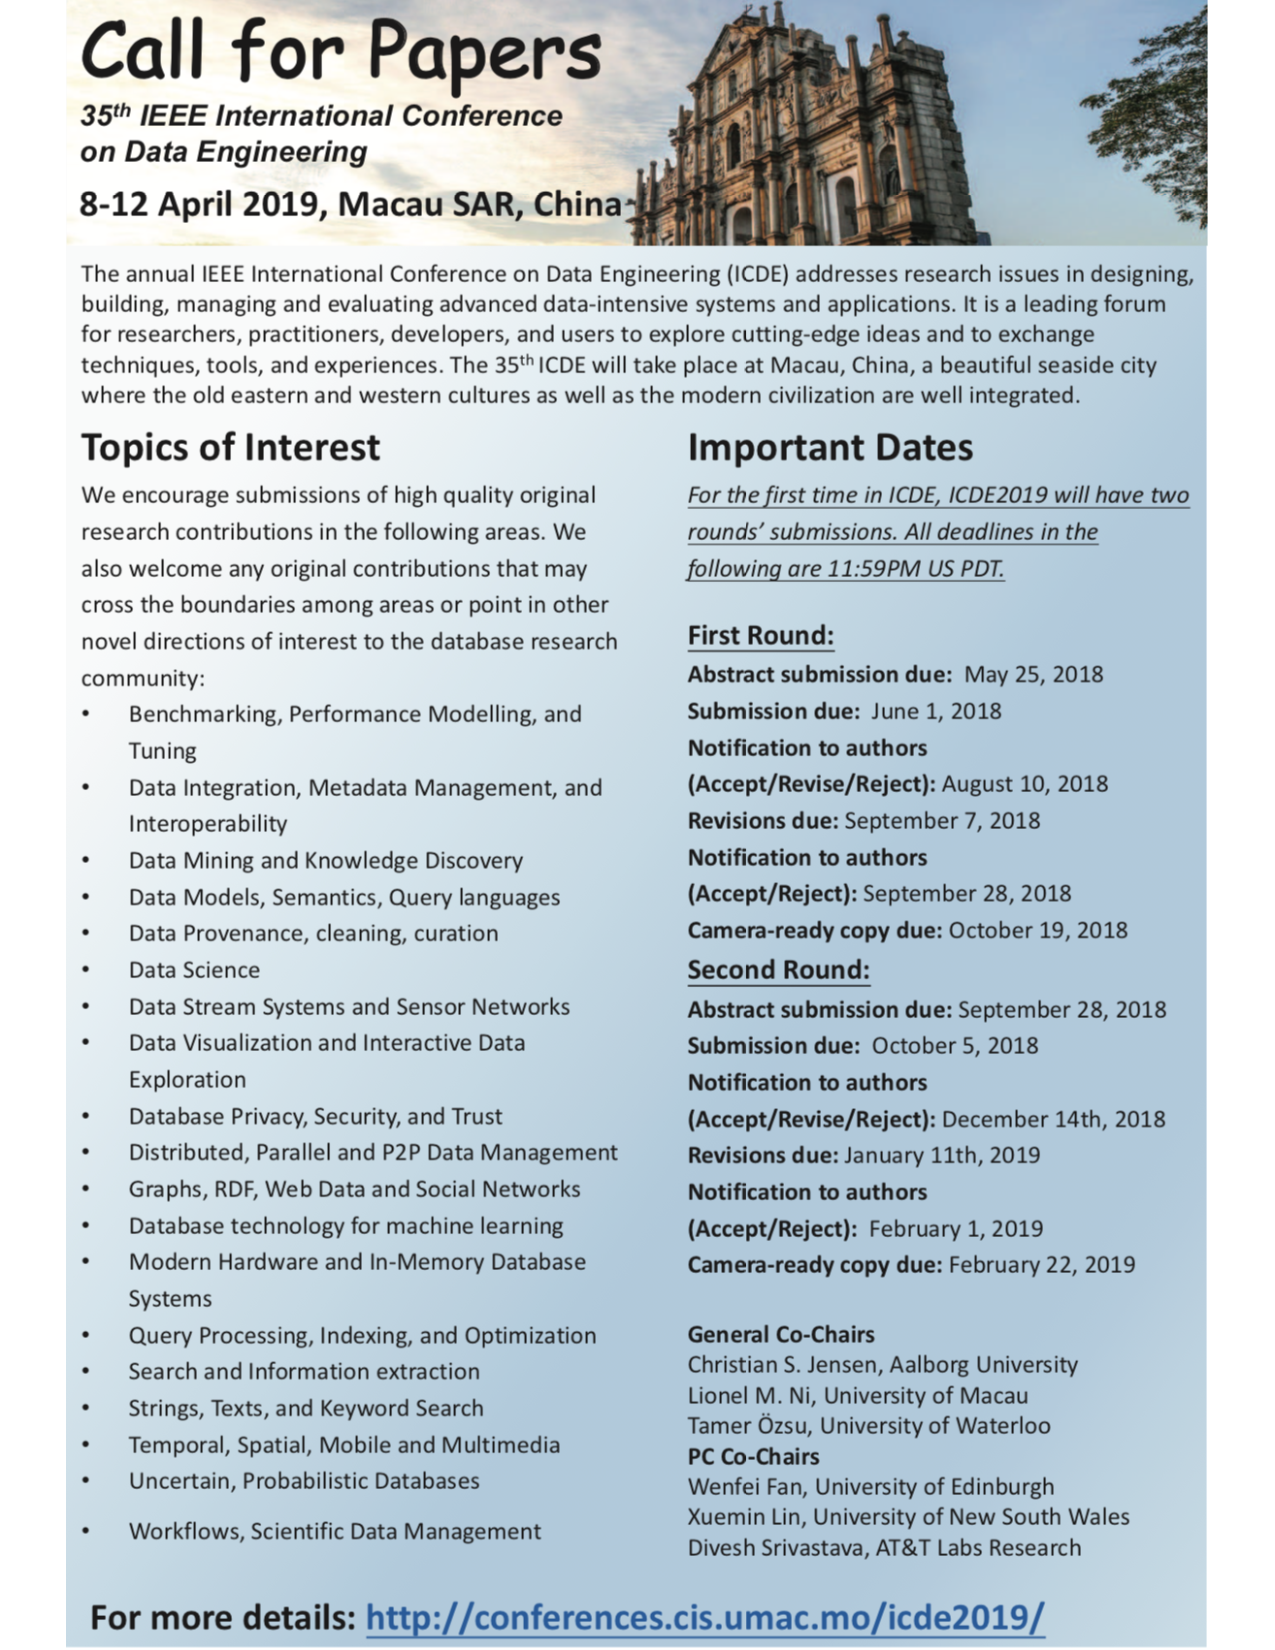
\includegraphics[width=\textwidth, bb= 0 0 610 790] {calls/icde19.pdf}} 
%\centerline{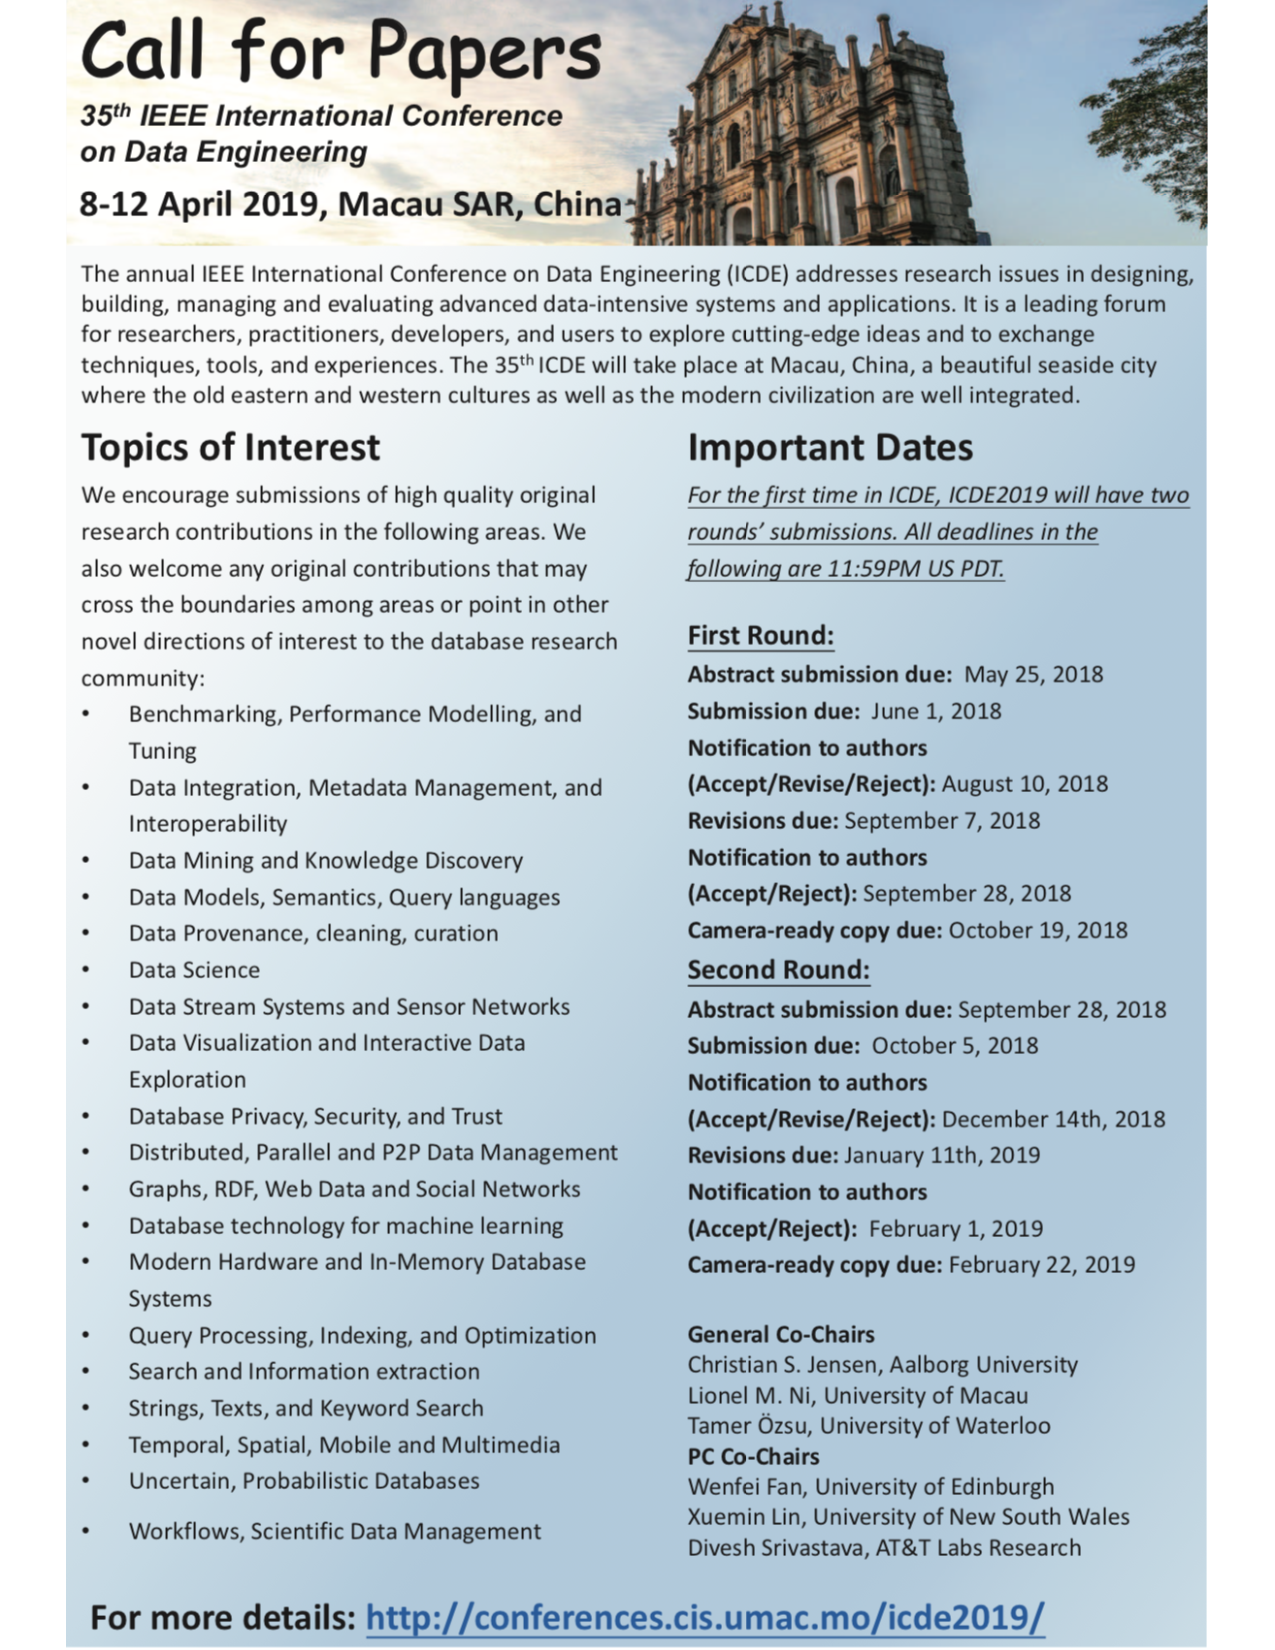
\includegraphics[width=\textwidth, bb= 0 0 590 760] {calls/icde19.pdf}}
\end{call}
\begin{call}{TCDE Membership Form}
%\centerline{\includegraphics[width=\textwidth, bb= 0 0 610 790]
\centerline{
\includegraphics[width=\textwidth, bb= 0 0 590 760] {calls/tcde.pdf}}
\end{call}
\end{callsection}

\end{bulletin}
\end{document}
